\documentclass[12pt,oneside]{book}

%%%%%%%%%%%%%%%%%%%%%%%%%%%%%%%%%%%%%%%%%%%%%%%%%%%%%%%%%%%%%%%%%%%%%%%%%%%%%%%%%%%%%%%%%%%%%%%%%%%
%                                                                                                 %
% The mathematical style of these documents follows                                               %
%                                                                                                 %
% A. Thompson and B.N. Taylor. The NIST Guide for the Use of the International System of Units.   %
%    NIST Special Publication 881, 2008.                                                          %
%                                                                                                 %
% http://www.nist.gov/pml/pubs/sp811/index.cfm                                                    %
%                                                                                                 %
%%%%%%%%%%%%%%%%%%%%%%%%%%%%%%%%%%%%%%%%%%%%%%%%%%%%%%%%%%%%%%%%%%%%%%%%%%%%%%%%%%%%%%%%%%%%%%%%%%%

% $Date: 2013-11-26 10:43:59 -0500 (Tue, 26 Nov 2013) $
% $Revision: 17538 $
% $Author: gforney $

%%%%%%%%%%%%%%%%%%%%%%%%%%%%%%%%%%%%%%%%%%%%%%%%%%%%%%%%%%%%%%%%%%%%%%%%%%%%%%%%%%%%%%%%%%%%%%%%%%%
%                                                                                                 %
% The mathematical style of these documents follows                                               %
%                                                                                                 %
% A. Thompson and B.N. Taylor. The NIST Guide for the Use of the International System of Units.   %
%    NIST Special Publication 881, 2008.                                                          %
%                                                                                                 %
% http://www.nist.gov/pml/pubs/sp811/index.cfm                                                    %
%                                                                                                 %
%%%%%%%%%%%%%%%%%%%%%%%%%%%%%%%%%%%%%%%%%%%%%%%%%%%%%%%%%%%%%%%%%%%%%%%%%%%%%%%%%%%%%%%%%%%%%%%%%%%

% Packages which force the use of better TeX coding
% Mostly from http://tex.stackexchange.com/q/19264
%%\RequirePackage[l2tabu, orthodox]{nag}
%%\usepackage{fixltx2e}
%\usepackage{isomath} % Disabled for the moment because it changes the syntax for bold and roman Greek math symbols
%%\usepackage[all,warning]{onlyamsmath}
%\usepackage{strict} % Commented out for now because it is uncommon. A copy of style.sty is in Manuals/LaTeX_Style_Files/.

\usepackage{times,mathptmx}
\usepackage[pdftex]{graphicx}
\usepackage{tabularx,ragged2e,booktabs,caption}
\usepackage{multirow}
\usepackage{pdfsync}
\usepackage{tikz}
\usepackage{pgfplots}
%\pgfplotsset{compat=1.7}
\usepackage{tocloft}
\usepackage{color}
\usepackage{amsmath}
\definecolor{linknavy}{rgb}{0,0,0.50196}
\definecolor{linkred}{rgb}{1,0,0}
\definecolor{linkblue}{rgb}{0,0,1}
\usepackage{float}
\usepackage{caption}
\usepackage{graphpap}
\usepackage{rotating}
\usepackage{graphicx}
\usepackage{geometry}
\usepackage{relsize}
\usepackage{longtable}
\usepackage{lscape}
\usepackage{amssymb}
\usepackage{makeidx} % Create index at end of document
\usepackage[nottoc,notlof,notlot]{tocbibind} % Put the bibliography and index in the ToC
\usepackage{lastpage} % Automatic last page number reference.
\usepackage[T1]{fontenc}
\usepackage{enumerate}
\usepackage{upquote}
\usepackage{moreverb}
\usepackage{xfrac}
\usepackage{cite}

\newcommand{\nopart}{\expandafter\def\csname Parent-1\endcsname{}} % To fix table of contents in pdf.
\newcommand{\ct}{\tt\small} % eventually will be deprecated due to http://www.tex.ac.uk/cgi-bin/texfaq2html?label=2letterfontcmd
\newcommand{\textct}[1]{\texttt{\small #1}}

\usepackage{tocstyle} % Fix table of contents sections from overlapping section titles
\usetocstyle{standard}
\usepackage{siunitx}
\sisetup{
    detect-all = true,
    input-decimal-markers = {.},
    input-ignore = {,},
    inter-unit-product = \ensuremath{{}\cdot{}},
    multi-part-units = repeat,
    number-unit-product = \text{~},
    per-mode = fraction,
    separate-uncertainty = true,
}

\usepackage{listings}
\usepackage{textcomp}
\definecolor{lbcolor}{rgb}{0.96,0.96,0.96}
\lstset{
    %backgroundcolor=\color{lbcolor},
    tabsize=4,
    rulecolor=,
    language=Fortran,
        basicstyle=\footnotesize\ttfamily,
        upquote=true,
        aboveskip={\baselineskip},
        belowskip={\baselineskip},
        columns=fixed,
        extendedchars=true,
        breaklines=true,
        breakatwhitespace=true,
        frame=none,
        showtabs=false,
        showspaces=false,
        showstringspaces=false,
        identifierstyle=\ttfamily,
        keywordstyle=\color[rgb]{0,0,0},
        commentstyle=\color[rgb]{0,0,0},
        stringstyle=\color[rgb]{0,0,0},
}

\usepackage[pdftex,
        colorlinks=true,
        urlcolor=linkblue,     % \href{...}{...} external (URL)
        citecolor=linkred,     % citation number colors
        linkcolor=linknavy,    % \ref{...} and \pageref{...}
        pdfproducer={pdflatex},
        pdfpagemode=UseNone,
        bookmarksopen=true,
        plainpages=false,
        verbose]{hyperref}

% The Following commented code makes the ``Draft'' watermark on each page.
%\usepackage{eso-pic}
%\usepackage{type1cm}
%\makeatletter
%   \AddToShipoutPicture{
%     \setlength{\@tempdimb}{.5\paperwidth}
%     \setlength{\@tempdimc}{.5\paperheight}
%     \setlength{\unitlength}{1pt}
%     \put(\strip@pt\@tempdimb,\strip@pt\@tempdimc){
%     \makebox(0,0){\rotatebox{45}{\textcolor[gray]{0.75}{\fontsize{8cm}\selectfont{RC6}}}}}
% }
%\makeatother

\setlength{\textwidth}{6.5in}
\setlength{\textheight}{9.0in}
\setlength{\topmargin}{0.in}
\setlength{\headheight}{0.pt}
\setlength{\headsep}{0.in}
\setlength{\parindent}{0.25in}
\setlength{\oddsidemargin}{0.0in}
\setlength{\evensidemargin}{0.0in}
\setlength{\leftmargini}{\parindent} % Controls the indenting of the "bullets" in a list
\setlength{\cftsecnumwidth}{0.45in}
\setlength{\cftsubsecnumwidth}{0.5in}
\setlength{\cftfignumwidth}{0.45in}
\setlength{\cfttabnumwidth}{0.45in}

\newcommand{\titlesigs}
{
\small
\flushright{U.S. Department of Commerce \\
{\em Penny Pritzker, Secretary} \\
\hspace{1in} \\
National Institute of Standards and Technology \\
{\em Willie May, Under Secretary of Commerce for Standards and Technology and Acting Director} }
}

% commands to use for "official" cover and title pages
% see smokeview verification guide to see how they are used

\newcommand{\headerA}[1]{
\flushright{
\fontsize{20}{24}\selectfont
\bf{NIST Special Publication #1}}
}

\newcommand{\headerB}[1]{
\flushright{
\fontsize{28}{33.6}\selectfont
\bf{#1}
}
}

\newcommand{\headerC}[1]{
\vspace{.5in}
\flushright{\fontsize{14}{16.8}\selectfont
#1}
}

\frenchspacing

\newcommand{\dod}[2]{\frac{\partial #1}{\partial #2}}
\newcommand{\DoD}[2]{\frac{\mathrm{D} #1}{\mathrm{D} #2}}
\newcommand{\dsods}[2]{\frac{\partial^2 #1}{\partial #2^2}}
\renewcommand{\d}{\,\mathrm{d}}
\newcommand{\dx}{\delta x}
\newcommand{\dy}{\delta y}
\newcommand{\dz}{\delta z}
\newcommand{\degF}{$^\circ$F}
\newcommand{\degC}{$^\circ$C}
\newcommand{\x}{x}
\newcommand{\y}{y}
\newcommand{\z}{z}
\newcommand{\dt}{\delta t}
\newcommand{\dn}{\delta n}
\newcommand{\cH}{H}
\newcommand{\hu}{u}
\newcommand{\hv}{v}
\newcommand{\hw}{w}
\newcommand{\la}{\lambda}
\newcommand{\bO}{{\Omega}}
\newcommand{\bo}{{\mathbf{\omega}}}
\newcommand{\btau}{\mathbf{\tau}}
\newcommand{\bdelta}{{\mathbf{\delta}}}
\newcommand{\sumyw}{\sum (Y_\alpha/W_\alpha)}
\newcommand{\oW}{\overline{W}}
\newcommand{\om}{\ensuremath{\omega}}
\newcommand{\omx}{\omega_x}
\newcommand{\omy}{\omega_y}
\newcommand{\omz}{\omega_z}
\newcommand{\erf}{\hbox{erf}}
\newcommand{\erfc}{\hbox{erfc}}
\newcommand{\bF}{{\mathbf{F}}}
\newcommand{\bG}{{\mathbf{G}}}
\newcommand{\bof}{{\mathbf{f}}}
\newcommand{\bq}{{\mathbf{q}}}
\newcommand{\br}{{\mathbf{r}}}
\newcommand{\bu}{{\mathbf{u}}}
\newcommand{\bx}{{\mathbf{x}}}
\newcommand{\bk}{{\mathbf{k}}}
\newcommand{\bv}{{\mathbf{v}}}
\newcommand{\bg}{{\mathbf{g}}}
\newcommand{\bn}{{\mathbf{n}}}
\newcommand{\bS}{{\mathbf{S}}}
\newcommand{\bW}{\overline{W}}
\newcommand{\dS}{d{\mathbf{S}}}
\newcommand{\bs}{{\mathbf{s}}}
\newcommand{\bI}{{\mathbf{I}}}
\newcommand{\hp}{H}
\newcommand{\trho}{\tilde{\rho}}
\newcommand{\dph}{{\delta\phi}}
\newcommand{\dth}{{\delta\theta}}
\newcommand{\tp}{\tilde{p}}
\newcommand{\bp}{\overline{p}}
\newcommand{\dQ}{\dot{Q}}
\newcommand{\dq}{\dot{q}}
\newcommand{\dbq}{\dot{\mathbf{q}}}
\newcommand{\dm}{\dot{m}}
\newcommand{\ha}{\frac{1}{2}}
\newcommand{\ft}{\frac{4}{3}}
\newcommand{\ot}{\frac{1}{3}}
\newcommand{\fofi}{\frac{4}{5}}
\newcommand{\of}{\frac{1}{4}}
\newcommand{\twth}{\frac{2}{3}}
\newcommand{\R}{R}
\newcommand{\be}{\begin{equation}}
\newcommand{\ee}{\end{equation}}
\newcommand{\RE}{\hbox{Re}}
\newcommand{\LE}{\hbox{Le}}
\newcommand{\PR}{\hbox{Pr}}
\newcommand{\PE}{\hbox{Pe}}
\newcommand{\NU}{\hbox{Nu}}
\newcommand{\SC}{\hbox{Sc}}
\newcommand{\SH}{\hbox{Sh}}
\newcommand{\WE}{\hbox{We}}
\newcommand{\COTWO}{\text{\tiny \hbox{CO}$_2$}}
\newcommand{\HTWOO}{\text{\tiny \hbox{H}$_2$\hbox{O}}}
\newcommand{\OTWO}{\text{\tiny \hbox{O}$_2$}}
\newcommand{\NTWO}{\text{\tiny \hbox{N}$_2$}}
\newcommand{\CO}{\text{\tiny \hbox{CO}}}
\newcommand{\F}{\text{\tiny \hbox{F}}}
\newcommand{\C}{\text{\tiny \hbox{C}}}
\newcommand{\Hy}{\text{\tiny \hbox{H}}}
\newcommand{\So}{\text{\tiny \hbox{S}}}
\newcommand{\M}{\text{\tiny \hbox{M}}}
\newcommand{\xx}{\text{\tiny \hbox{x}}}
\newcommand{\yy}{\text{\tiny \hbox{y}}}
\newcommand{\zz}{\text{\tiny \hbox{z}}}
\newcommand{\smvlines}{115~000}

\newcommand{\calH}{\mathcal{H}}
\newcommand{\calR}{\mathcal{R}}

\newcommand{\dif}{\mathrm{d}}
\newcommand{\Div}{\nabla\cdot}
\newcommand{\D}{\mbox{D}}
\newcommand{\mhalf}{\mbox{$\frac{1}{2}$}}
\newcommand{\thalf}{\mbox{\tiny $\frac{1}{2}$}}
\newcommand{\tripleprime}{{\prime\prime\prime}}
\newcommand{\ppp}{{\prime\prime\prime}}
\newcommand{\pp}{{\prime\prime}}

\newcommand{\superscript}[1]{\ensuremath{^{\textrm{\tiny #1}}}}
\newcommand{\subscript}[1]{\ensuremath{_{\textrm{\tiny #1}}}}

\newcommand{\rb}[1]{\raisebox{1.5ex}[0pt]{#1}}

\newcommand{\Ra}{$\Rightarrow$}
\newcommand{\hhref}[1]{\href{#1}{{\tt #1}}}
\newcommand{\fdsinput}[1]{{\scriptsize\verbatiminput{../../Verification/Visualization/#1}}}

\definecolor{AQUAMARINE}{rgb}{0.49804,1.00000,0.83137}
\definecolor{ANTIQUE WHITE}{rgb}{0.98039,0.92157,0.84314}
\definecolor{BEIGE}{rgb}{0.96078,0.96078,0.86275}
\definecolor{BLACK}{rgb}{0.00000,0.00000,0.00000}
\definecolor{BLUE}{rgb}{0.00000,0.00000,1.00000}
\definecolor{BLUE VIOLET}{rgb}{0.54118,0.16863,0.88627}
\definecolor{BRICK}{rgb}{0.61176,0.40000,0.12157}
\definecolor{BROWN}{rgb}{0.64706,0.16471,0.16471}
\definecolor{BURNT SIENNA}{rgb}{0.54118,0.21176,0.05882}
\definecolor{BURNT UMBER}{rgb}{0.54118,0.20000,0.14118}
\definecolor{CADET BLUE}{rgb}{0.37255,0.61961,0.62745}
\definecolor{CHOCOLATE}{rgb}{0.82353,0.41176,0.11765}
\definecolor{COBALT}{rgb}{0.23922,0.34902,0.67059}
\definecolor{CORAL}{rgb}{1.00000,0.49804,0.31373}
\definecolor{CYAN}{rgb}{0.00000,1.00000,1.00000}
\definecolor{DIMGRAY }{rgb}{0.41176,0.41176,0.41176}
\definecolor{EMERALD GREEN}{rgb}{0.00000,0.78824,0.34118}
\definecolor{FIREBRICK}{rgb}{0.69804,0.13333,0.13333}
\definecolor{FLESH}{rgb}{1.00000,0.49020,0.25098}
\definecolor{FOREST GREEN}{rgb}{0.13333,0.54510,0.13333}
\definecolor{GOLD }{rgb}{1.00000,0.84314,0.00000}
\definecolor{GOLDENROD}{rgb}{0.85490,0.64706,0.12549}
\definecolor{GRAY}{rgb}{0.50196,0.50196,0.50196}
\definecolor{GREEN}{rgb}{0.00000,1.00000,0.00000}
\definecolor{GREEN YELLOW}{rgb}{0.67843,1.00000,0.18431}
\definecolor{HONEYDEW}{rgb}{0.94118,1.00000,0.94118}
\definecolor{HOT PINK}{rgb}{1.00000,0.41176,0.70588}
\definecolor{INDIAN RED}{rgb}{0.80392,0.36078,0.36078}
\definecolor{INDIGO}{rgb}{0.29412,0.00000,0.50980}
\definecolor{IVORY}{rgb}{1.00000,1.00000,0.94118}
\definecolor{IVORY BLACK}{rgb}{0.16078,0.14118,0.12941}
\definecolor{KELLY GREEN}{rgb}{0.00000,0.50196,0.00000}
\definecolor{KHAKI}{rgb}{0.94118,0.90196,0.54902}
\definecolor{LAVENDER}{rgb}{0.90196,0.90196,0.98039}
\definecolor{LIME GREEN}{rgb}{0.19608,0.80392,0.19608}
\definecolor{MAGENTA}{rgb}{1.00000,0.00000,1.00000}
\definecolor{MAROON}{rgb}{0.50196,0.00000,0.00000}
\definecolor{MELON}{rgb}{0.89020,0.65882,0.41176}
\definecolor{MIDNIGHT BLUE}{rgb}{0.09804,0.09804,0.43922}
\definecolor{MINT}{rgb}{0.74118,0.98824,0.78824}
\definecolor{NAVY}{rgb}{0.00000,0.00000,0.50196}
\definecolor{OLIVE}{rgb}{0.50196,0.50196,0.00000}
\definecolor{OLIVE DRAB}{rgb}{0.41961,0.55686,0.13725}
\definecolor{ORANGE}{rgb}{1.00000,0.50196,0.00000}
\definecolor{ORANGE RED}{rgb}{1.00000,0.27059,0.00000}
\definecolor{ORCHID}{rgb}{0.85490,0.43922,0.83922}
\definecolor{PINK}{rgb}{1.00000,0.75294,0.79608}
\definecolor{POWDER BLUE}{rgb}{0.69020,0.87843,0.90196}
\definecolor{PURPLE}{rgb}{0.50196,0.00000,0.50196}
\definecolor{RASPBERRY}{rgb}{0.52941,0.14902,0.34118}
\definecolor{RED}{rgb}{1.00000,0.00000,0.00000}
\definecolor{ROYAL BLUE}{rgb}{0.25490,0.41176,0.88235}
\definecolor{SALMON}{rgb}{0.98039,0.50196,0.44706}
\definecolor{SANDY BROWN}{rgb}{0.95686,0.64314,0.37647}
\definecolor{SEA GREEN}{rgb}{0.32941,1.00000,0.62353}
\definecolor{SEPIA}{rgb}{0.36863,0.14902,0.07059}
\definecolor{SIENNA}{rgb}{0.62745,0.32157,0.17647}
\definecolor{SILVER}{rgb}{0.75294,0.75294,0.75294}
\definecolor{SKY BLUE}{rgb}{0.52941,0.80784,0.92157}
\definecolor{SLATEBLUE}{rgb}{0.41569,0.35294,0.80392}
\definecolor{SLATE GRAY}{rgb}{0.43922,0.50196,0.56471}
\definecolor{SPRING GREEN}{rgb}{0.00000,1.00000,0.49804}
\definecolor{STEEL BLUE}{rgb}{0.27451,0.50980,0.70588}
\definecolor{TAN}{rgb}{0.82353,0.70588,0.54902}
\definecolor{TEAL}{rgb}{0.00000,0.50196,0.50196}
\definecolor{THISTLE}{rgb}{0.84706,0.74902,0.84706}
\definecolor{TOMATO }{rgb}{1.00000,0.38824,0.27843}
\definecolor{TURQUOISE}{rgb}{0.25098,0.87843,0.81569}
\definecolor{VIOLET}{rgb}{0.93333,0.50980,0.93333}
\definecolor{VIOLET RED}{rgb}{0.81569,0.12549,0.56471}
\definecolor{WHITE}{rgb}{1.00000,1.00000,1.00000}
\definecolor{YELLOW}{rgb}{1.00000,1.00000,0.00000}

\pgfplotsset{
	colormap={blackwhite}{[5pt]
		rgb255(0pt)=(0,0,255); 
		rgb255(100pt)=(0,255,255); 
		rgb255(200pt)=(0,255,0); 
		rgb255(300pt)=(255,255,0); 
		rgb255(400pt)=(255,0,0)
	},
} % defines smokeview colorbar


\floatstyle{boxed}
\newfloat{notebox}{H}{lon}
\newfloat{warning}{H}{low}

% Set default longtable alignment
\setlength\LTleft{0pt}
\setlength\LTright{0pt}


% Rename chapter headings
\renewcommand{\chaptername}{Section}
\renewcommand{\bibname}{References}

% Math shortcuts
\renewcommand{\sb}[1]{_\mathrm{#1}}
\renewcommand{\C}{\mbox{C}}
\renewcommand{\H}{\mbox{H}}
\renewcommand{\O}{\mbox{O}}
\newcommand{\N}{\mbox{N}}

% Center all figures
\makeatletter
\g@addto@macro\@floatboxreset\centering
\makeatother

% Extra packages
\usepackage{xfrac}

\begin{document}
	
\bibliographystyle{unsrt}
\pagestyle{empty}
	
\begin{minipage}[t][9in][s]{6.25in}
	
\begin{flushright}
\fontsize{20}{24}\selectfont
\bf{NIST Technical Note XXXX}
\end{flushright}
		
\headerB{
Delaware County, PA Fire Suppression Tests \\
Spring 2012 \\
}
		
\normalsize
		
\headerC{
{
\flushright{
Daniel Madrzykowski \\
Keith M. Stakes \\
					
\vspace*{2\baselineskip}
				
\begingroup
This publication is available free of charge from:
\hypersetup{urlcolor=black}
\href{http://dx.doi.org/10.6028/NIST.TN.XXXX}{http://dx.doi.org/10.6028/NIST.TN.XXXX}
\endgroup
}
				
\vfill
				
\flushright{
		

\includegraphics[width=2.in]{../../../Bibliography/nistident_flright_vec} \\[.3in]
}
}
}
		
\end{minipage}

\newpage
\hspace{5in}
\newpage
	
\frontmatter
	
\pagenumbering{roman}
	
\begin{minipage}[t][9in][s]{6.25in}
		
\begin{flushright}
\fontsize{20}{24}\selectfont
\bf{NIST Technical Note XXXX}
\end{flushright}
		
\headerB{
Delaware County, PA Fire Suppression Tests \\
Spring 2012 \\
}
		
\headerC{
\flushright{
Daniel Madrzykowski \\
Keith M. Stakes \\
{\em Fire Research Division \\
Engineering Laboratory} \\
				
\vspace*{2\baselineskip}
				
\begingroup
This publication is available free of charge from:
\hypersetup{urlcolor=black}
\href{http://dx.doi.org/10.6028/NIST.TN.XXXX}{http://dx.doi.org/10.6028/NIST.TN.XXXX} \\
\endgroup
				
\vspace*{2\baselineskip}
August 2014}}
		
\vfill
		
\flushright{
\includegraphics[width=1in]{../../../Bibliography/doc} }
	
\titlesigs
		
\end{minipage}
	
\newpage
	
\begin{minipage}[t][9in][s]{6.25in}
		
\flushright{Certain commercial entities, equipment, or materials may be identified in this \\
document in order to describe an experimental procedure or concept adequately. \\
Such identification is not intended to imply recommendation or endorsement by the \\
National Institute of Standards and Technology, nor is it intended to imply that the \\
entities, materials, or equipment are necessarily the best available for the purpose. \\
}
		
\vspace{3in}
		
\large
\flushright{\bf National Institute of Standards and Technology Technical Note XXXX \\
Natl.~Inst.~Stand.~Technol.~Tech.~Note~XX, \pageref{LastPage} pages (August 2014) \\
% http://dx.doi.org/10.6028/NIST.TN.XXXX \\
CODEN: NTNOEF }

\vspace{0.2in}

\begingroup
{\bf This publication is available free of charge from:}
\hypersetup{urlcolor=black}
\href{http://dx.doi.org/10.6028/NIST.TN.1838}{\bf http://dx.doi.org/10.6028/NIST.TN.1838} \\
\endgroup		

\vfill
		
\hspace{1in}
		
\end{minipage}
	
\newpage
	
\frontmatter
	
\pagestyle{plain}
\pagenumbering{roman}
	
\cleardoublepage
\phantomsection
\addcontentsline{toc}{chapter}{Contents}
\tableofcontents
	
\cleardoublepage
\phantomsection
\addcontentsline{toc}{chapter}{List of Figures}
\listoffigures
	
\cleardoublepage
\phantomsection
\addcontentsline{toc}{chapter}{List of Tables}
\listoftables
	
\chapter{List of Acronyms}
	
\begin{tabbing}
\hspace{1.5in} \= \\
FDS \> Fire Dynamics Simulator \\
HGL \> Hot Gas Layer \\
HRR \> Heat Release Rate \\
HRRPUA \> Heat Release Rate per Unit Area \\
NIST \> National Institute of Standards and Technology \\
\end{tabbing}
	
\mainmatter
	
\chapter{Abstract}
\label{chap:Abstract} 



\chapter{Introduction}
\label{chap:Introduction}

NIST FFTG

Objective: To improve the safety and effectiveness of firefighters through measurement science to advance suppression tactics, examine non-traditional means of fire suppression, and transfer of the results to the fire service. 

Aid the fire service across the country in the most effective and safe way to fight fires.

The goal is to improve the safety of not only the responding firefighters but the public as well through the use of modern fire suppression tactics for modern fires.

Approach: Real scale, instrumented fire suppression experiments. 

This is an STRS project that has been complemented with OA studies funding from: 
Cal Poly 
FDNY 
ISFSI 
NYU 

NIST has conducted a significant amount of research examining how ventilation affects the growth and spread of fire within structures and how the air flow to the fire may be controlled to limit or delay the growth of the fire.  The studies have resulted in guidance to the fire service regarding ventilation tactics.  However ventilation tactics alone will not result in the complete extinguishment of the fire, fire suppression with hose streams are needed.

Fire suppression tactics using hose streams also affect the ventilation in a structure and can impact the movement of smoke and heat through a structure as vents are made to advance the line or if ventilation inducing hand line tactics are in practice.  This research addressing the coordination of suppression tactics and the impact on ventilation is needed to complete recommendations on fire control tactics to appropriate standards, education, and training documents.

Test Objectives:

1)	Examine the water distribution for solid streams, straight streams, and fog streams.

2)	Examine the impact of solid streams, straight streams, and fog streams on the cooling of fire gases inside a structure with various flow path configurations, structure configurations, and structure volumes.

Constants: 
Building Geometry
Fuel Load
Fire Room Conditions at time of water flow
Water Flow Rate – 120 gpm

Variable: 
Smooth Bore vs Narrow Fog


\chapter{Experimental Setup}
\label{chap:Experimental_Setup}

WATER DISTRIBUTION

Purpose:
- Determine the appropriate location for nozzles
- Determine water distribution

Setup:
Task Force Tips Metro 1, Fixed Gallonage (120 gpm)
Straight Stream
30 degree Fog
7/8” Smooth Bore
100 ft of 1-3/4 inch hose

The hose streams were from fixed monitor nozzles simulating a firefighter with the hose line in the structure.

Controlled and operated via a gate valve from the exterior.

12 Experiments:
4 SS from room
2 Fog from room
2 SS from Hall
2 Fog from Hall
1 SB from Hall
1 SB from Room

2.5 square foot collector bin.

Bins were poly boxes with interlacing lips to prevent water from going in between.

Measured how much of the water ended up in what part of the room.

The building was sheathed in plastic for the water flow tests as to protect and preserve the structure before any fire suppression tests were conducted.

Spray Distribution Summary:
- Experiments provided nozzle placement for gas cooling and fire suppression experiments.
- Provide a sense of the distribution of the water throughout the test space.

Hallway nozzle = gas cooling

Room nozzle = seat of fire

FIRE SUPPRESSION

Room and contents fire inside structure
Two points of interior attack
- Remotely activated in hallway (indirect attack)
- Remotely activated in fire room (direct attack)

Common household furnishings.

Due to the limited time and resources for testing, the extremes were chosen: smooth bore and narrow fog.

Straight stream from a fog nozzle was the medium between the two.



\section{Experimental Facility}
\label{sec:Experimental_Facility}

\subsection{Burn Building - Gas Cooling}
\label{sec:Burn_Building}

\begin{figure}[!ht]
	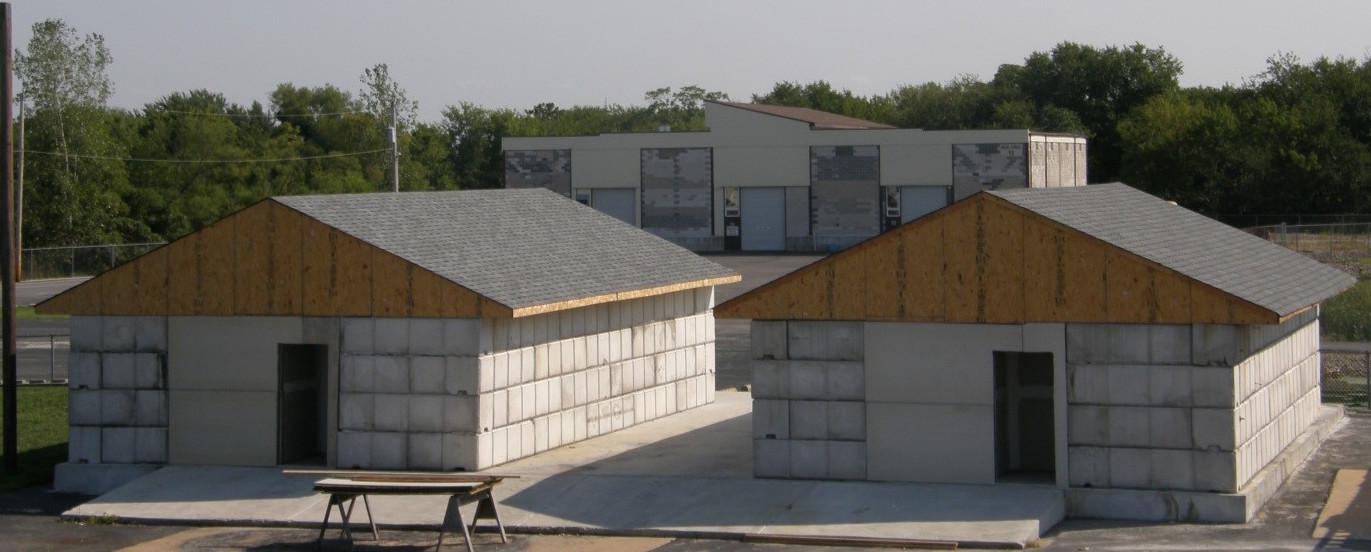
\includegraphics[width=6in]{../Figures/Pictures/DelCo_Structures}
	\caption{Delaware County, PA Fire Test Structures}
	\label{fig:Delaware_County,_PA_Fire_Test_Structures}
\end{figure}

\subsection{Concrete Structures - Fire Suppression}
\label{sec:Experimental Structures}

Two identical concrete structures were built on a concrete slab as shown in Fig.~\ref{sec:Experimental_Facility}. They were designed to simulate a single floor of a residential structure.  The outer wall of each structure was composed of interlocking concrete blocks 0.61 m (2 ft) wide, 0.61 m (2 ft) high and 1.22 m (4 ft) long.  The interior dimensions of teach structure were 6.1 m (20 ft) wide, 11 m (36 ft) long and 2.4 m (8 ft) high.  The joints and gaps between the blocks were filled with high temperature insulation.

\begin{figure}[!ht]
	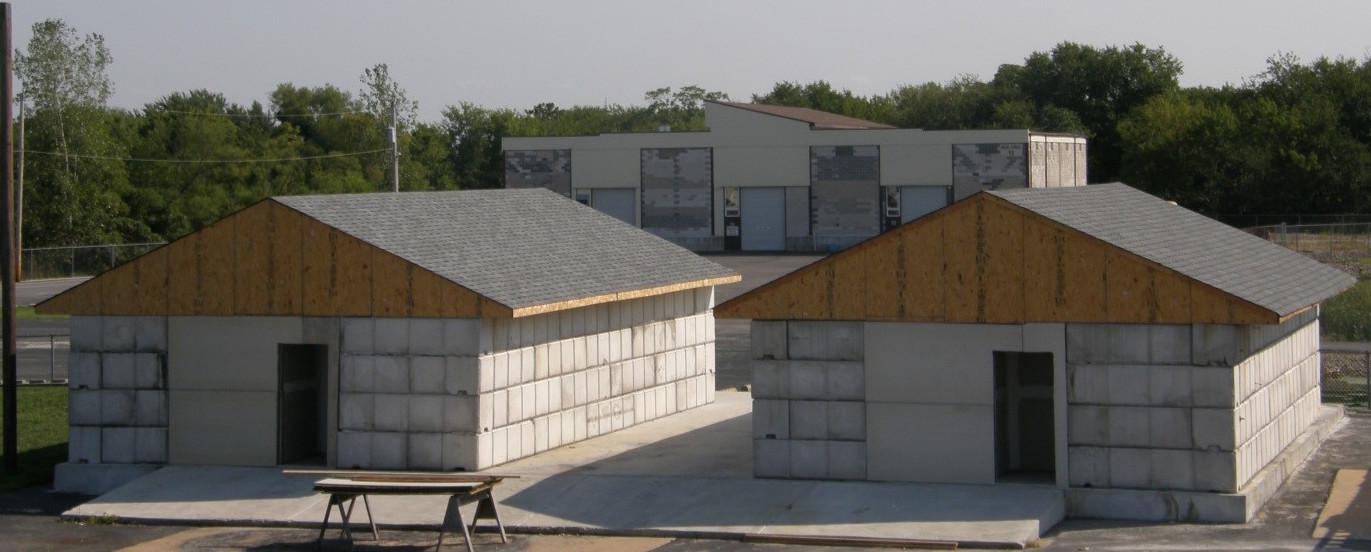
\includegraphics[width=6in]{../Figures/Pictures/DelCo_Structures}
	\caption{Delaware County, PA Fire Test Structures}
	\label{fig:Delaware_County,_PA_Fire_Test_Structures}
\end{figure}

Each structure had burn room, approximately 6.0 m (19.6 ft) by 4.4 m (14.3 ft) and 2.74 m (9.0 ft) in height and a hallway connecting the burn room to the front of the structure via a small entry foyer.  The hallway is approximately 0.95 m (3.1 ft) wide and 5.4 m (17.6 ft) and the entry foyer is 1.2 m (4.1 ft) by 1.9 m (6.1 ft).  The ceiling height in the hallway and entry foyer was 2.4 m (8 ft).  The open door on north side from the exterior to the entry foyer was 2.0 m (6.5 ft) high and 0.9 m (2.9 ft) wide.  The opening on the south face of the structure from the exterior to the burn room was 2.4 m (7.75 ft) high and 1.09 m (3.6 ft) wide.   A schematic plan view of the structure is given in Figure     .    

\begin{figure}[!ht]
	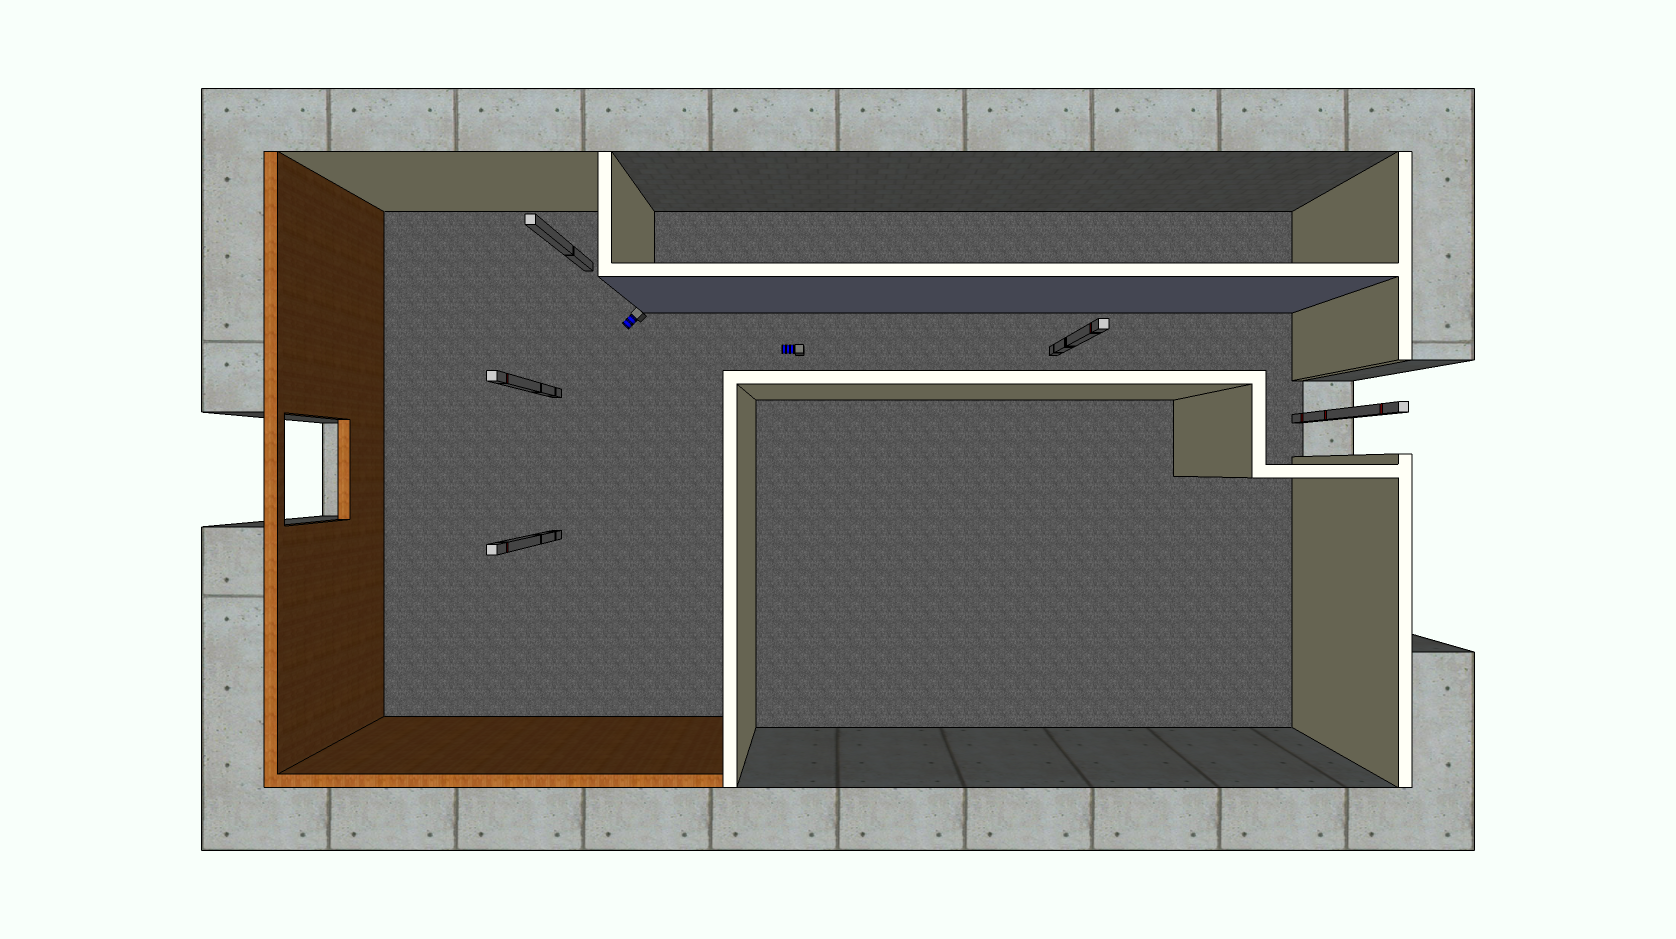
\includegraphics[width=6in]{../Figures/Pictures/DelCoSingleStory}
	\caption{Delaware County, PA Fire Test Structure}
	\label{fig:DelCoSingleStory}
\end{figure}

\begin{figure}[!ht]
	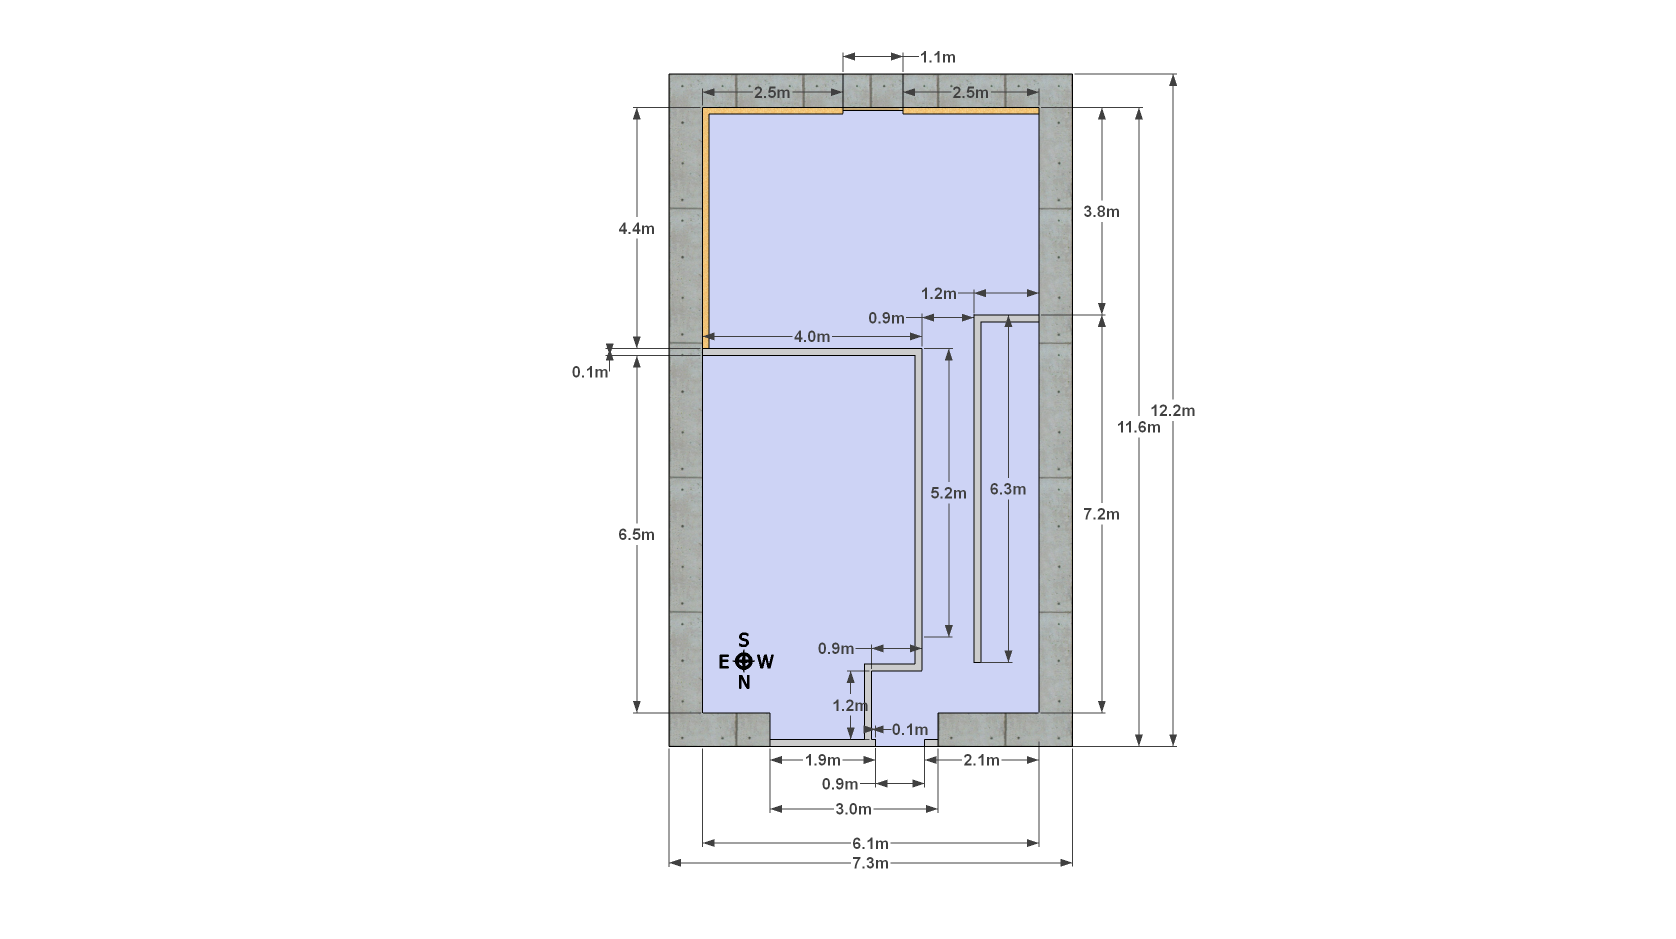
\includegraphics[width=6in]{../Figures/Pictures/DelCoSingleStoryDimensionsMetric}
	\caption{Floor Plan of the Test Structure.}
	\label{fig:Test_Structure_Floor_Plan}
\end{figure}

The floor of the structure was a concrete pad.  The interior walls of the structure were framed with steel studs and track.  The studs were set to 0.40 m (16 in) centers.  The ceiling support was composed of wood truss joist I-beams (TJIs) with a 299 mm (11.75 in) depth.  The TJI was composed of laminated veneer lumber flanges with a cross section of 29 mm (1.125 in) x 44 mm (1.75 in) and an 11 mm (0.43 in) thick oriented strand board web as shown in .  Tongue and grove, 18.3 mm (0.72 in) thick, oriented strand board was attached to the top of the TJIs.     

The interior walls of the burn room were lined with 13 mm (0.5 in) thick cement board.  The ceiling of the burn room was the exposed ``floor assembly".  The walls of the hallway and entry foyer were composed of 16 mm (0.625 in) Type X gypsum room. The ceiling of the hallway and entry foyer was composed of two layers of 13 mm (0.5 in) thick cement board.    

Both structures were similar and were used to run comparative experiments on a given day.

\section{Instrumentation}
\label{sec:Instrumentation}

\subsection{Gas Cooling Instrumentation} 
\label{subsec:Gas_Cooling_Instrumentation}

\begin{figure}[!ht]
	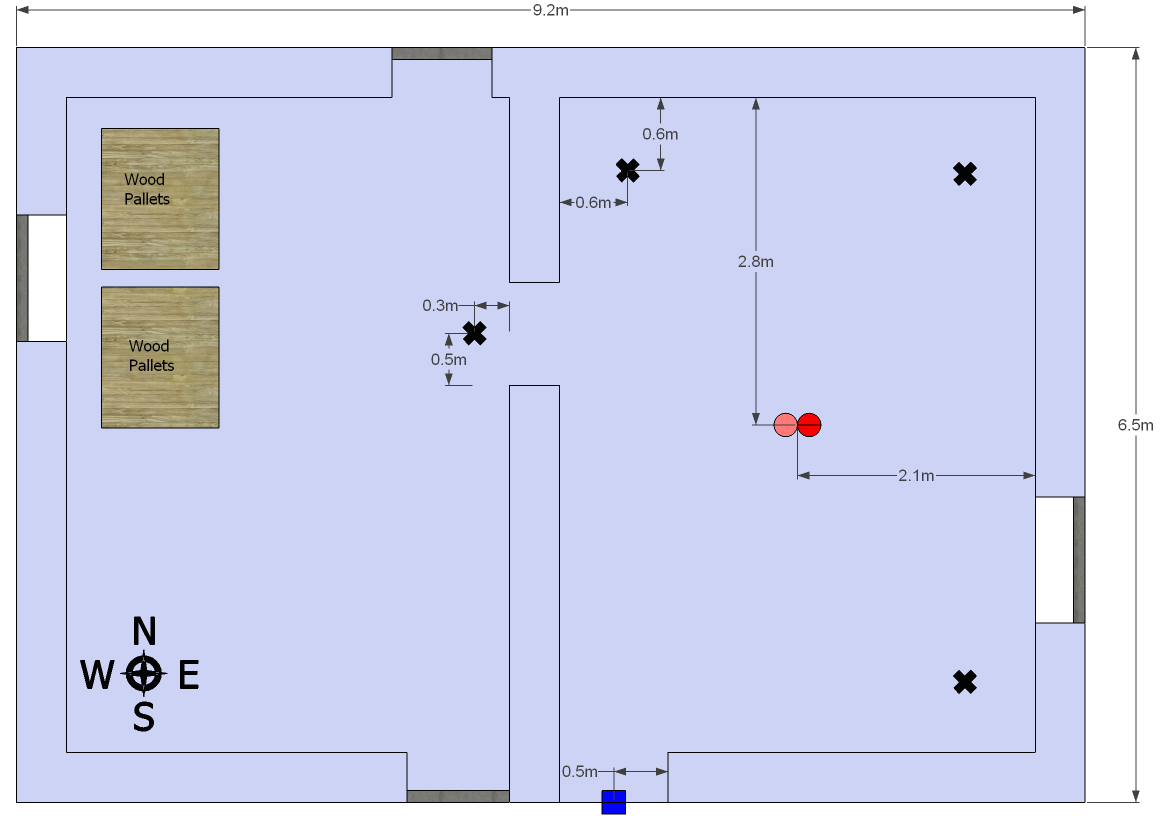
\includegraphics[width=6in]{../Figures/Pictures/DelCoBurnBuildingInstrumentation}
	\caption{Photograph of the Instrumentation Dimensions in the Gas Cooling Experiments}
	\label{fig:Gas_Cooling_Instrumentation_Dimensions}
\end{figure}

\subsection{Fire Suppression Instrumentation}
\label{subsec:Fire_Suppression_Instrumentation}

The structures were instrumented for temperature, heat flux, and gas velocity measurements.  A schematic plan view of the instrumentation arrangement is show in ???? 

\begin{figure}[!ht]
	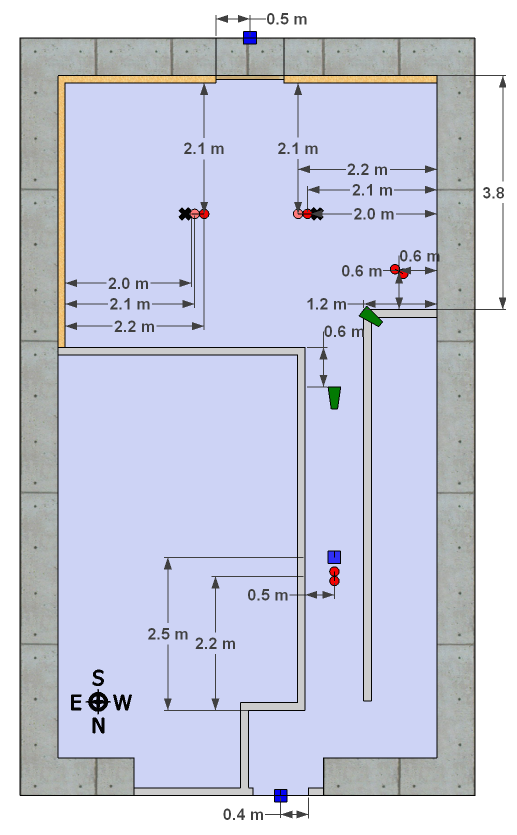
\includegraphics[width=6in]{../Figures/Pictures/DelCoSingleStoryInstrumentationDimensions}
	\caption{Photograph of the Instrumentation Dimensions in the Fire Suppression Experiments.}
	\label{fig:Fire_Suppression_Instrumentation_Dimensions}
\end{figure}

\begin{figure}[!ht]
	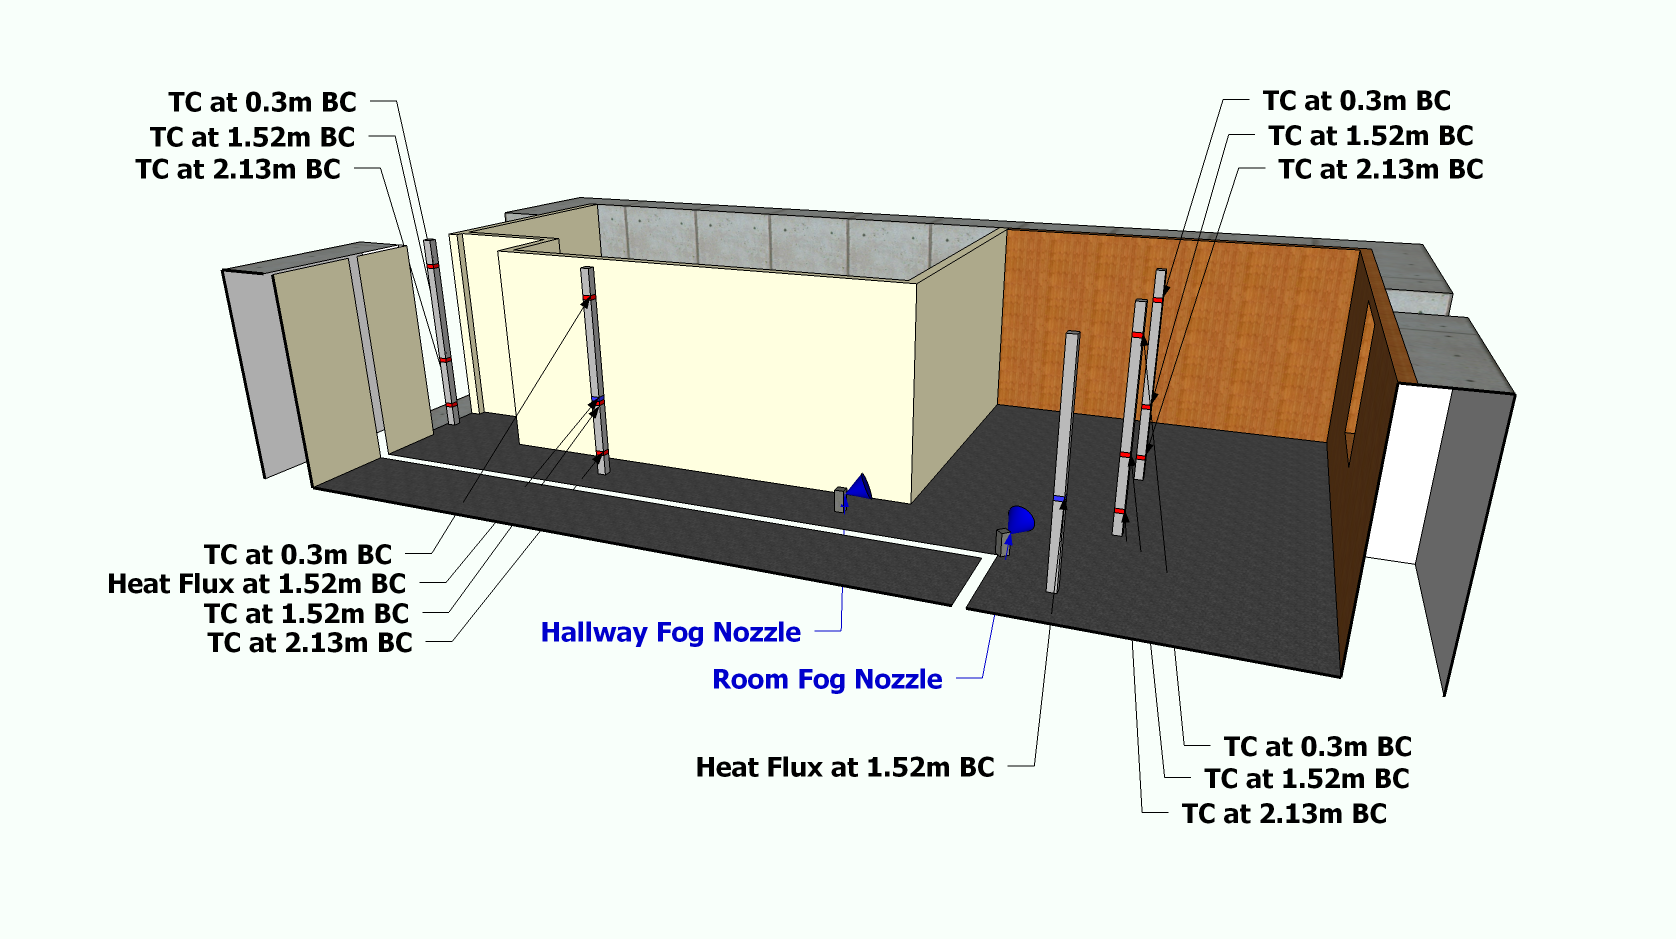
\includegraphics[width=6in]{../Figures/Pictures/Fog_Instrumentation}
	\caption{Photograph of the Instrumentation in the Fog Stream Tests.}
	\label{fig:Fog_Instrumentation}
\end{figure}

\begin{figure}[!ht]
	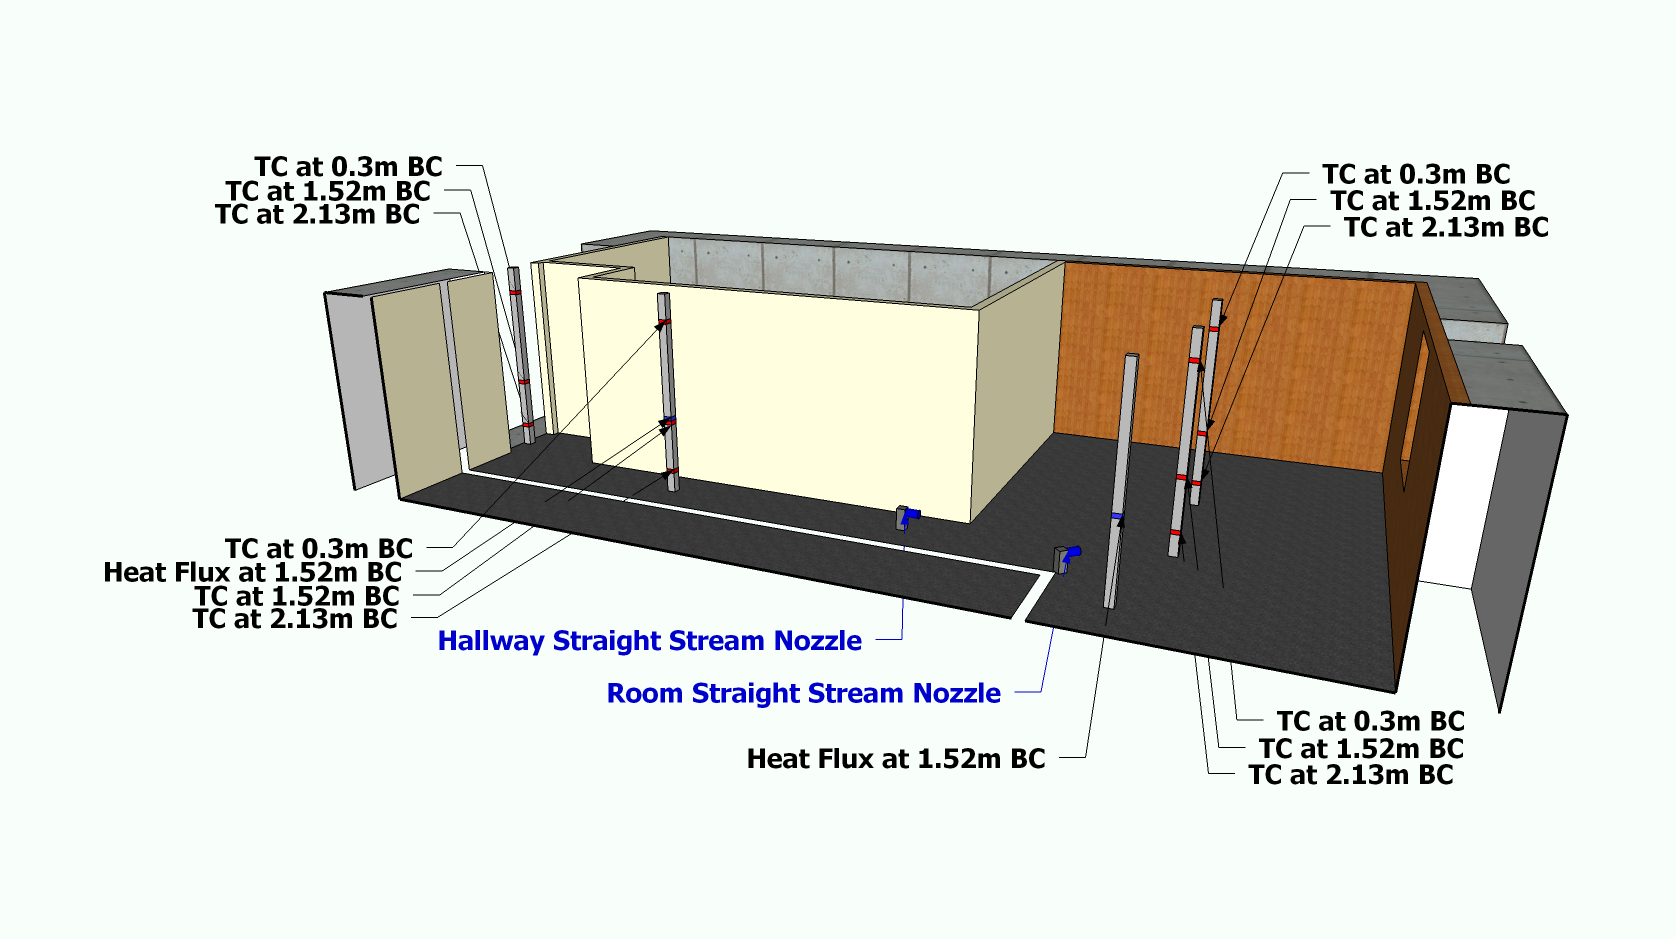
\includegraphics[width=6in]{../Figures/Pictures/Straight_Stream_Instrumentation}
	\caption{Photograph of the Instrumentation in the Straight Stream Tests.}
	\label{fig:Straigh_Stream_Instrumentation}
\end{figure}

\subsection{Temperature}
\label{subsec:Temperature}

Thermocouples:
Work through the Seebeck effect.  Two dissimilar metals are joined together with a weld bead.  Each metal generates a voltage, different from one another, when exposed to a thermal gradient.  This voltage difference increases with an increase in energy to the thermocouple and through a correlation, a corresponding temperature is found.  

\subsubsection{Gas Cooling Experiments}
\label{subsubsec:Gas_Cooling_Temperature_Instrumentation}

\subsubsection{Fire Suppression Experiments}
\label{subsubsec:Fire_Suppression_Temperature_Instrumentation}

Gas temperatures in the burn room were measured with bare-bead, Chromel-Alumel (type K) thermocouples, with a 0.5 mm (0.02 in) nominal diameter.  Thermocouple arrays were installed 2.0 m (6.7 ft) from both the east and the west walls of the burn room and 2.1 m (6.9 ft) from the south wall as shown in Figure ..  The vertical arrays had thermocouples located 0.03, 0.3, 0.61, 0.91, 1.22, 1.52, 1.83, 2.13 m below the bottom edge of the joist, where a ceiling would be installed.   

Additional single thermocouples were installed in conjunction with the bi-directional probes at the exterior vents and in the hallway.  The single thermocouples were bare-bead, Chromel-Alumel (type K) thermocouples, with a 1.0 mm (0.04 in) nominal diameter. Just behind the bead, the thermocouple wire is protected with an 3.2 mm (0.125 in) diameter inconel sheath.  
In the north doorway, there were seven thermocouples were located at: 0.15 m (0.5 ft), 0.30 m (1 ft), 0.61 m (2 ft), 0.91 m (3 ft), 1.22 m (4 ft), 1.51 m (5.0 ft), and 1.83 (6.0 ft) below the soffit along the vertical centerline of the doorway opening.  In the hallway, there were seven thermocouples positioned vertically at: 0.15 m (0.5 ft), 0.30 m (1 ft), 0.61 m (2 ft), 0.91 m (3 ft), 1.22 m (4 ft), 1.51 m (5.0 ft), and 1.83 (6.0 ft)   In the south window opening, there were four thermocouples are located 0.28 m (0.95 ft), 0.58 (1.90 ft), 0.84 m (2.85 ft), and 1.16 m (3.8 ft) below the soffit.  

\subsection{Heat Flux}
\label{subsec:Heat_Flux}

Total Heat Flux:
Water cooled heat flux gauges measure both the convective and radiative heat transfer to the sensor.  Hot and cold side of a plate simulating the hot and cold side of a thermocouple.  The temperature gradient generates a voltage and through correlations, a total heat flux measurement is obtained.  The sensor is water cooled to ensure a thermal gradient remains and the sensor does not reach uniform temperature.  The sensor top is painted black to assist with radiation absorption.

Radiometer:
The radiometer is simply a total heat flux gauge with Zirconium plate atop the sensor preventing the device from recording any heat due to convective transfer.


\subsubsection{Gas Cooling Experiments}
\label{subsubsec:Gas_Cooling_Heat_Flux_Instrumentation}

\subsubsection{Fire Suppression Experiments}
\label{subsubsec:Fire_Suppression_Heat_Flux_Instrumentation}

Total heat flux was measured with Schmidt Boelter gauges.  Radiant heat flux was measured with Schmidt Boelter gauges with sapphire lens.  One of each was located near the thermocouple arrays in the burn room.  The gauges were pointed at the ceiling and positioned 0.15 m (6 in) above the floor.  

In the northwest corner of the burn room two total heat flux gauges are located approximately 0.61 m (2 ft) out of the corner and 1.52 m (5 ft) below the ceiling, a position chosen to be representative of the height of a crawling firefighter's head.  One of the gauge's sensing surface is facing the ceiling and the other gauge is facing the pallets.  A similar heat flux gauge installation is located in the hallway, approximately 3.81 m (12.5 ft) from the burn room and 0.3 m (1ft) from the east wall of the hallway as shown in figure xx.  Again on gauge was facing the ceiling and one was facing the burn room.  

\subsection{Gas Velocity}
\label{subsec:Gas_Velocity}

Bi-directional Probes:
- Fire flow measurements are taken using these devices which have a high and low pressure side.  These flows then travel to a pressure transducer.  Through a simple conversion, the voltages are converted to pressure and finally a velocity based on the pressure and corresponding temperature measurements.

\subsubsection{Gas Cooling Experiments}
\label{subsubsec:Gas_Cooling_Gas_Velocity_Instrumentation}

\subsubsection{Fire Suppression Experiments}
\label{subsubsec:Fire_Suppression_Gas_Velocity_Instrumentation}

Gas velocity was determined utilizing differential pressure transducers connected to bidirectional velocity probes[ ] in conjunction with a temperature measurement.  These probes were co-located with the sheathed thermocouples in the north doorway, the south window opening and the hallway.  The locations are shown in ??????

\subsection{Mass}
\label{subsec:Mass}

\subsection{Moisture Content}
\label{subsec:Moisture_Content}

\subsection{Infrared Radiation}
\label{subsec:Infrared_Radiation}

\subsection{Uncertainty}
\label{subsec:Uncertainty}



\section{Fuel Load: Gas Cooling}
\label{sec:Fuel_Load:_Gas_Cooling} 

\begin{figure}[!ht]
	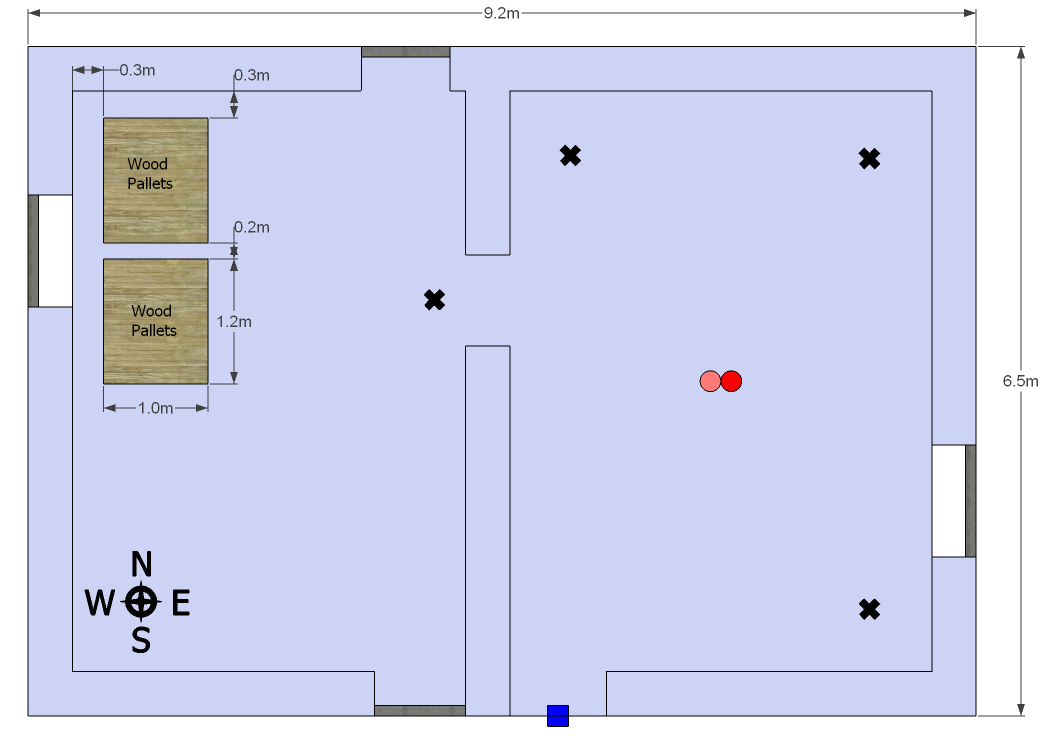
\includegraphics[width=6in]{../Figures/Pictures/DelCoBurnBuildingFuelLoad}
	\caption{Burn Building Fuel Load.}
	\label{fig:Burn_Building_Fuel_Load}
\end{figure}

\section{Fuel Load: Wood Experiments}
\label{sec:Fuel_Load:_Wood_Experiments} 

The fuel load for the experiments consisted of one bale of hay, twelve pallets, eleven and a half sheets plywood on the walls and the wood ``floor assembly". Two stacks of pallets with hay were used as the first items ignited in each experiment.  Each stack was composed of six pallets with a half bale of hay.  The hay was layered between each pallet.  The pallets and hay were weighed prior to each experiment.  For the four experiments, the average mass of the two stacks of pallets and the bale of hay was 232.4~kg (511.3~lb).  A complete listing of the mass of each pallet and hay bales is given in Appendix ????????
  
The pallet stacks were located 0.3~m (12~in) away from the east and south walls of the burn room.  The pallets were 1.2~m (48~in) long, 1.0~m (40~in) and 123~mm (4.8~in) high.  The stacks were 150~mm (6~in) apart.  One layer of 13 mm (0.5 in) thick gypsum board panels were laid on the concrete floor under the wood pallets to form a protective layer to minimize thermal damage to the concrete floor.
The east and south wall of the burn room was covered with 15~mm (0.59~in) thick, sheets of plywood.  The ``wood flooring assembly", composed of 12 TGIs and 9 sheets of OSB, served as the ceiling of the burn room.  The open doorway to the burn room on the south side was covered with a 2.4~m (8~ft) tall by 1.2~m (4~ft) wide piece of medium density fiberboard paneling that was 5~mm (0.19~in) thick.  The southeast corner of the burn room with the fuel load installed is shown in Fig.~\ref{fig:Wood_Fuel_Load}.

\begin{figure}[!ht]
	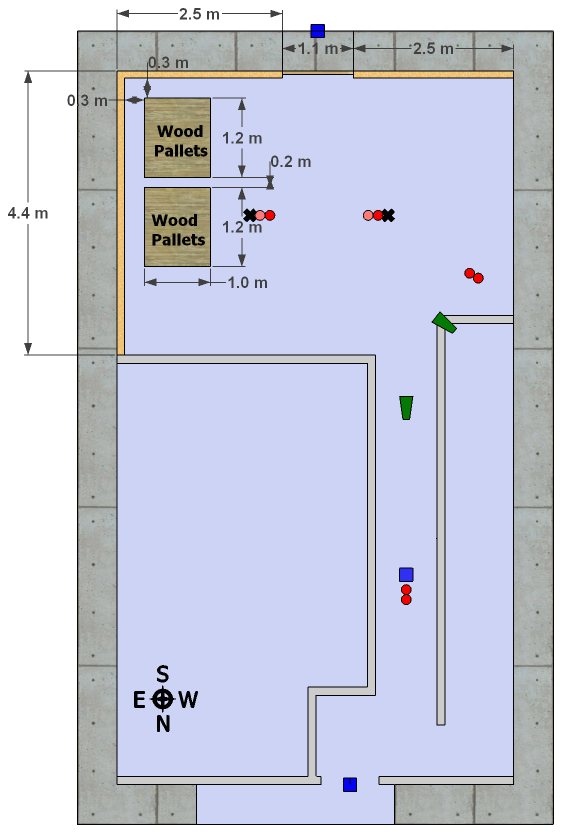
\includegraphics[width=6in]{../Figures/Pictures/DelCoSingleStoryWoodFuelLoad}
	\caption{Wood Fuel Load Dimensions.}
	\label{fig:Wood_Fuel_Load_Dimensions}
\end{figure}

\begin{figure}[!ht]
	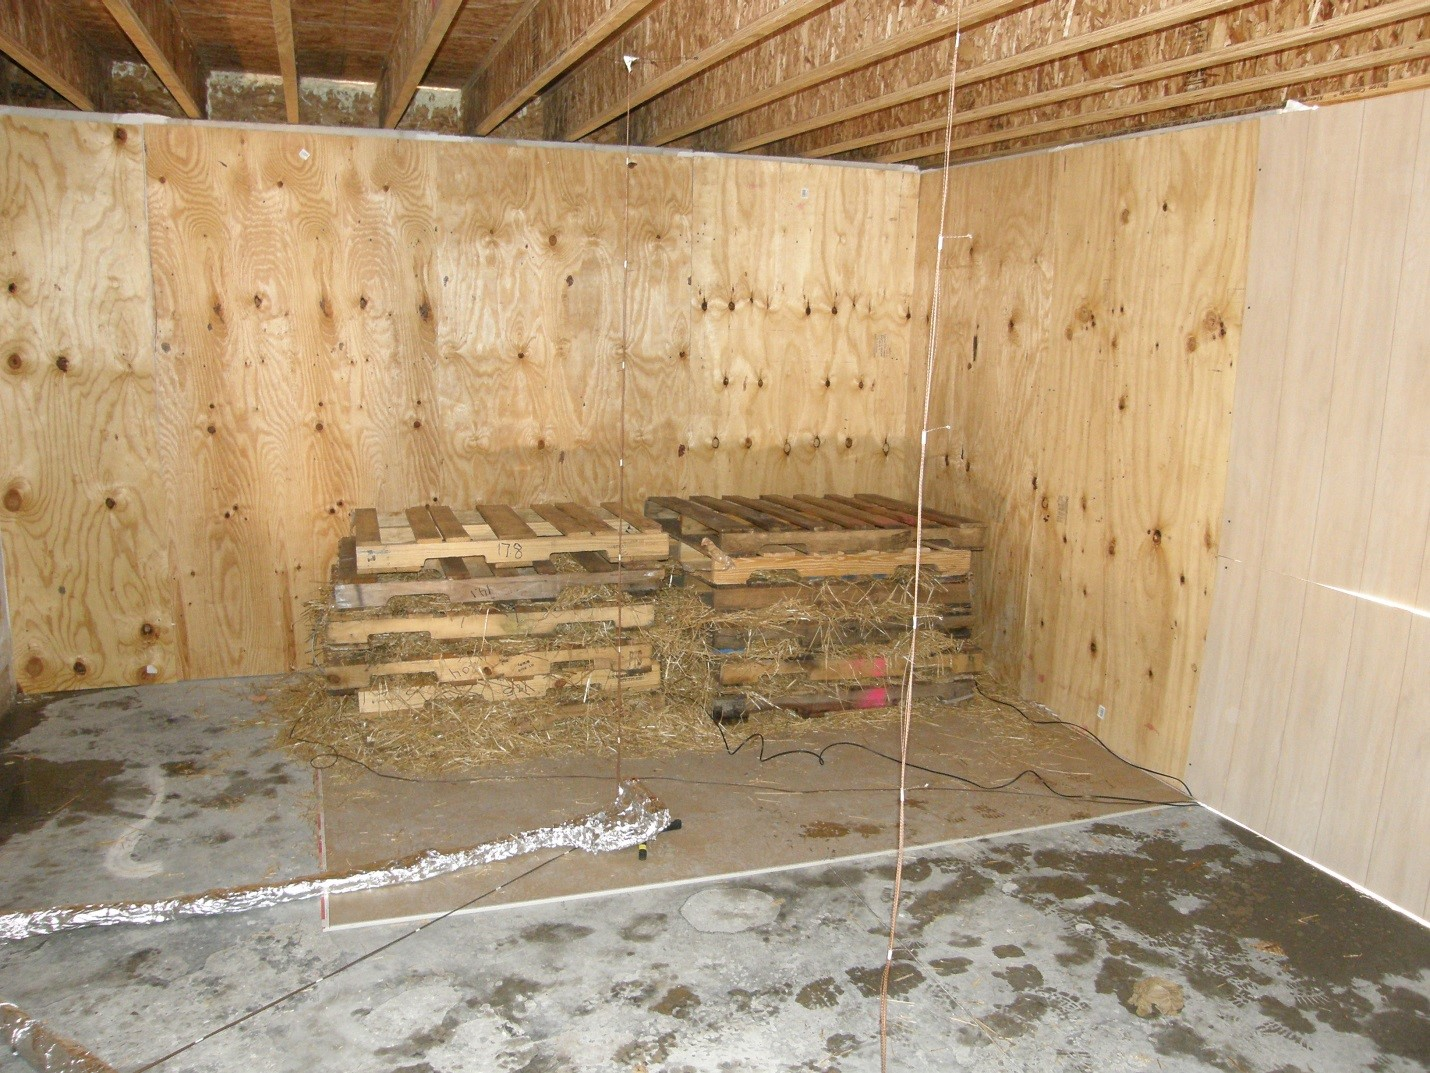
\includegraphics[width=6in]{../Figures/Pictures/Wood_Fuel_Package}
	\caption{Photograph of Southeast corner of burn room with wood fuel load.}
	\label{fig:Wood_Fuel_Load}
\end{figure}

\section{Fuel Load: Furniture Experiments}
\label{sec:Fuel_Load:_Furniture_Experiments}

\begin{figure}[!ht]
	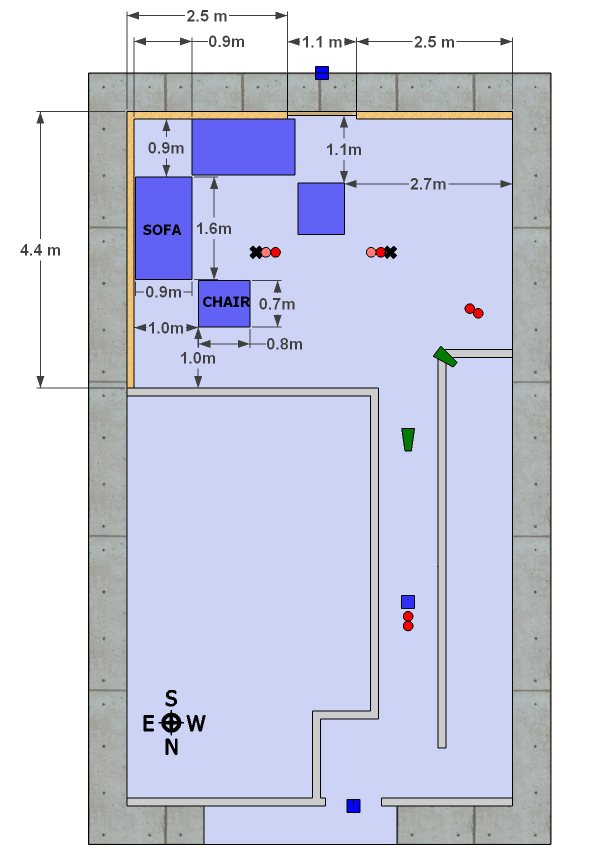
\includegraphics[width=6in]{../Figures/Pictures/DelCoSingleStoryFurnitureFuelLoad}
	\caption{Furniture Fuel Load Dimensions.}
	\label{fig:Furniture_Fuel_Load_Dimensions}
\end{figure}

\begin{sidewaystable}[!ht]
	\centering
	\caption{Fuel masses}
	\begin{tabular}{llcc}
		\hline\noalign{\smallskip}
		Item                         &  Material Description             &  Dimensions (m)            &  Mass (kg)  \\
		\noalign{\smallskip}\hline\noalign{\smallskip}
		3-seat Legacy Sofa         &  491 Brawley                      &  1.96 m x 0.86 m x 0.89 m  &  56.2 kg    \\
		Cushion (left)           &  Cotton w/ inner springs          &                            &  4.06 kg    \\
		Cushions (center)        &  Cotton w/ inner springs          &                            &  4.56 kg    \\
		Cushions (rear)          &  Cotton w/ inner springs          &                            &  4.16 kg    \\
		2-seat New Sofa            &  491 Brawley                      &  1.59 m x 0.91 m x 0.86 m  &  33.3 kg    \\
		Cushion (seat)           &                                   &  0.56 m x 0.61 m x 0.14 m  &  1.6 kg     \\
		Cushion (rear)           &  0.71 m at top, 0.58 m at bottom  &  Varies x 0.53 m x 0.20 m  &  2.0 kg     \\
		3-seat Brown Sofa            &  302 College (front room)         &  2.24 m x 1.02 m x 0.91 m  &  61.0 kg    \\
		2-seat Purple Stripe Sofa    &  302 College (front room)         &  1.57 m x 0.97 m x 0.86 m  &  82.0 kg    \\
		3-seat Black Pine Leaf Sofa  &  302 College (front room)         &  2.08 m x 0.86 m x 0.86 m  &  51.0 kg    \\
		Blue/Brown Chair             &  302 College (front room)         &  0.97 m x 0.81 m x 0.97 m  &  46.4 kg    \\
		2-seat Floral Sofa           &  302 College (rear room)          &  1.68 m x 0.91 m x 0.91 m  &  34.5 kg    \\
		2-seat Blue Plaid Sofa       &  302 College (rear room)          &  1.63 m x 0.97 m x 0.91 m  &  39.8 kg    \\
		3-seat Yellow Sofa           &  302 College (rear room)          &  2.13 m x 0.91 m x 0.71 m  &  48.3 kg    \\
		3-seat Floral Sofa           &  302 College (rear room)          &  2.29 m x 0.91 m x 0.91 m  &  48.0 kg    \\
		3-seat New Sofa              &  289 College (front room)         &  2.13 m x 0.91 m x 0.91 m  &  43.0 kg    \\
		Blue Chair                   &  289 College (middle room)        &  0.91 m x 0.91 m x 0.91 m  &  25.3 kg    \\
		3-seat Floral Sofa           &  289 College (sprinkler room)     &  2.24 m x 1.02 m x 1.02 m  &  81.2 kg    \\
		Floral Chair                 &  289 College (sprinkler room)     &  1.02 m x 1.02 m x 1.02 m  &  36.3 kg    \\
		\noalign{\smallskip}\hline
	\end{tabular}
	\label{tab:Fuel_Masses}
\end{sidewaystable}

\chapter{Experiments and Results}
\label{chap:Experiments_and_Results}

\section{Gas Cooling}
\label{sec:Gas_Cooling}

\subsection{Spray Density}
\label{subsec:Spray_Density}

\section{Fire Suppression}
\label{sec:Fire_Suppression}	

\begin{sidewaystable}[!ht]
	\centering
	\caption{Test Descriptions}
	\begin{tabular}{lllll}
		\hline\noalign{\smallskip}
		Test		& Agent		& Stream				& Flow Rate			& Comments \\
		\noalign{\smallskip}\hline\noalign{\smallskip}
		1 (FSE1)    &  CAF      &  30 deg Fog  			&  120 gpm/60 cfm   &	Furniture Fuel Package  \\
		2 (FSW2)   	& Water     &  30 deg Fog  			&  120 gpm    		&	Furniture Fuel Package	\\
		3 (FSW3) 	&  CAF      &  7/8" Smooth Bore  	&  120 gpm/60 cfm   &	Furniture Fuel Package  \\
		4 (FSE4)    &  Water    &  7/8" Smooth Bore  	&  120 gpm    		&	Furniture Fuel Package	\\
		5 (FSE5)    &  Water    &  30 deg Fog  			&  120 gpm    		&	Furniture Fuel Package	\\
		6 (FSW6)    &  CAF      &  30 deg Fog  			&  120 gpm/60 cfm   &	Furniture Fuel Package  \\
		7 (FSW7)    &  Water    &  30 deg Fog  			&  120 gpm    		&	Furniture Fuel Package	\\
		8 (FSE8)    &  CAF      &  30 deg Fog  			&  120 gpm/60 cfm   &	Furniture Fuel Package  \\
		9 (Attic 1) &  Water    &  Straight Stream  	&  120 gpm    		&	Furniture Fuel Package	\\
		10 (Attic 2)&  CAF      &  Straight Stream  	&  120 gpm/60 cfm   &	Furniture Fuel Package  \\
		11 (FSE1)   &  Water    &  30 deg Fog  			&  120 gpm   		&	Wood Fuel Package, Panel Window	 \\
		12 (FSW1)   &  CAF      &  30 deg Fog  			&  120 gpm/60 cfm   &	Wood Fuel Package, Panel Window  \\
		13 (FSE2)   &  Water    &  30 deg Fog  			&  120 gpm    		&	Wood Fuel Package, Panel Window  \\
		14 (FSW2)   &  CAF      &  30 deg Fog  			&  120 gpm/60 cfm   &	Wood Fuel Package, Panel Window  \\
		\noalign{\smallskip}\hline
	\end{tabular}
	\label{tab:Test_Descriptions}
\end{sidewaystable}

\begin{sidewaystable}[!ht]
	\centering
	\caption{Nozzle Activation Times}
	\begin{tabular}{lllllll}
		\hline\noalign{\smallskip}
		Test		& Agent		& Stream				& Nozzle 1 Activation	& Nozzle 1 Shut Off		& Nozzle 2 Activation	& Nozzle 2 Shut Off \\
		\noalign{\smallskip}\hline\noalign{\smallskip}
		1 (FSE1)    &  CAF      &  30 deg Fog  	    	& 233 					& 248					& 269					& 284					\\
		2 (FSW2)   	& Water     &  30 deg Fog  	    	& 235					& 250					& 272					& 287					\\
		3 (FSW3) 	&  CAF      &  7/8" Smooth Bore     & 228					& 243 					& 255					& 270					\\
		4 (FSE4)    &  Water    &  7/8" Smooth Bore     & 233					& 248					& 268					& 283					\\
		5 (FSE5)    &  Water    &  30 deg Fog  	    	& 232					& 247					& 257					& 272					\\
		6 (FSW6)    &  CAF      &  30 deg Fog     		& 239					& 254					& 268					& 283					\\
		7 (FSW7)    &  Water    &  30 deg Fog     		& 276					& 291					& 308					& 323					\\
		8 (FSE8)    &  CAF      &  30 deg Fog     		& 245					& 260					& 275					& 290					\\
		9 (Attic 1) &  Water    &  Straight Stream     	&						&						&						&					\\
		10 (Attic 2)&  CAF      &  Straight Stream     	& 						&						&						&					\\
		11 (FSE1)   &  Water    &  30 deg Fog  	   		& 315					& 330					& 345					& 360					\\
		12 (FSW1)   &  CAF      &  30 deg Fog  	   		& 233					& 248					& 263					& 278					\\
		13 (FSE2)   &  Water    &  30 deg Fog  	   		& 330					& 390					& 406					& 466					\\
		14 (FSW2)   &  CAF      &  30 deg Fog  	  		& 435					& 495					& 510					& 570					\\
		\noalign{\smallskip}\hline
	\end{tabular}
	\label{tab:Nozzle_Activation_Times}
\end{sidewaystable}
	
\subsection{Wood Fuel Package}
\label{subsec:Wood_Fuel_Package}

\begin{figure}[!ht]
	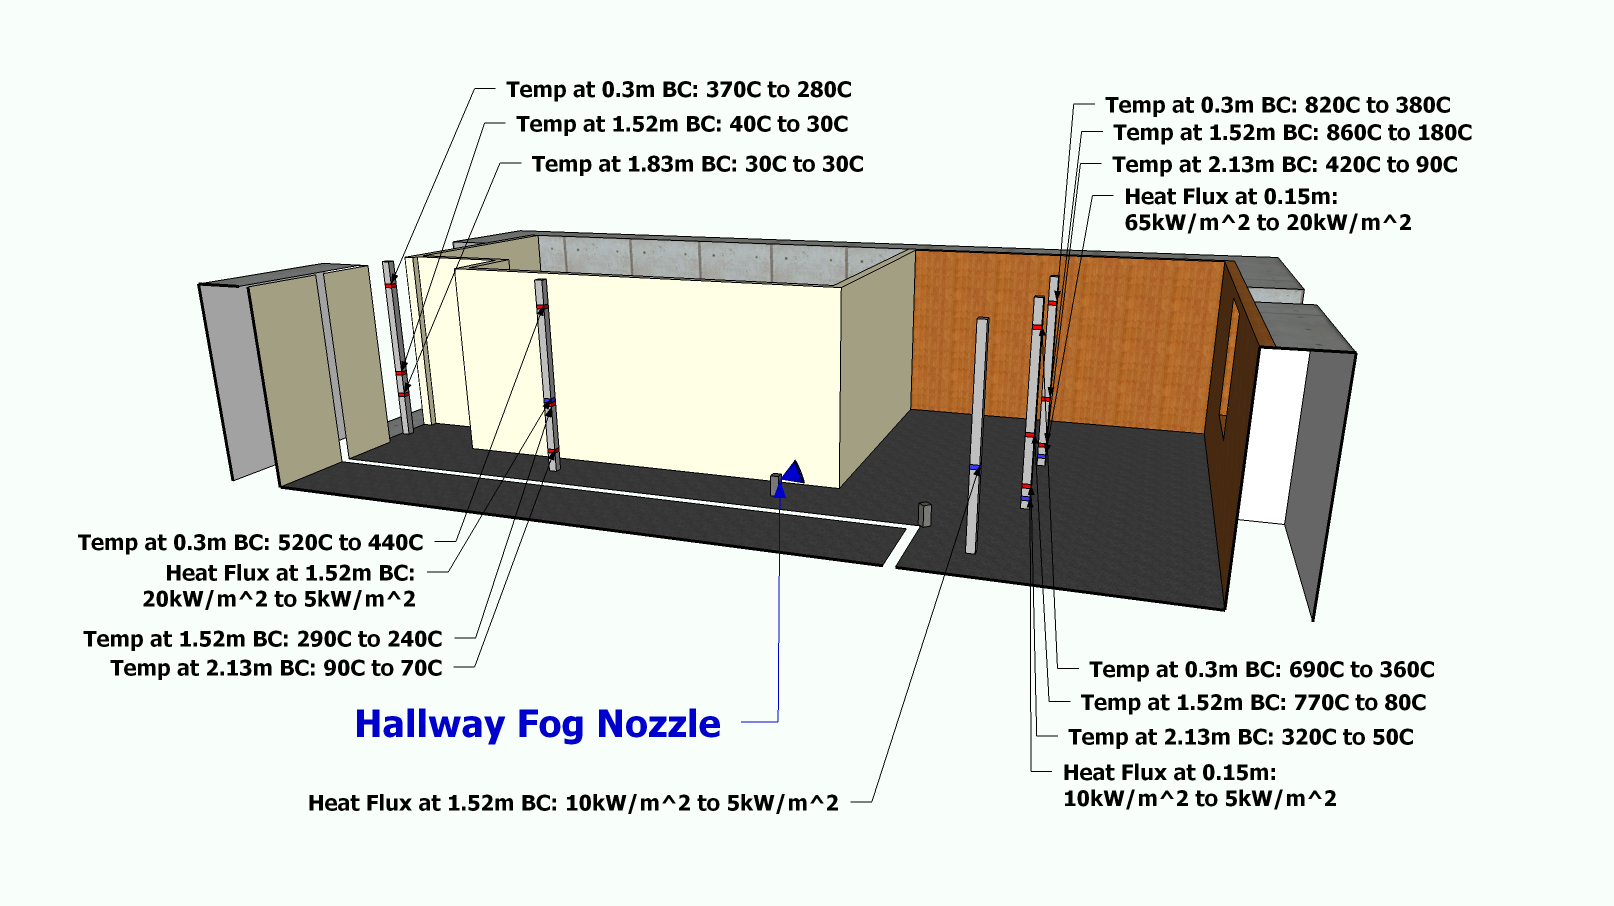
\includegraphics[width=6in]{../Figures/Pictures/Metric/DelCoFogTest11FirstSuppression}
	\caption{Test 11: Wood Fuel Package, Panel Window, Water, 30 deg Fog, 120 gpm, First Suppression}
	\label{fig:Test_11_First_Suppression}
\end{figure}

\begin{figure}[!ht]
	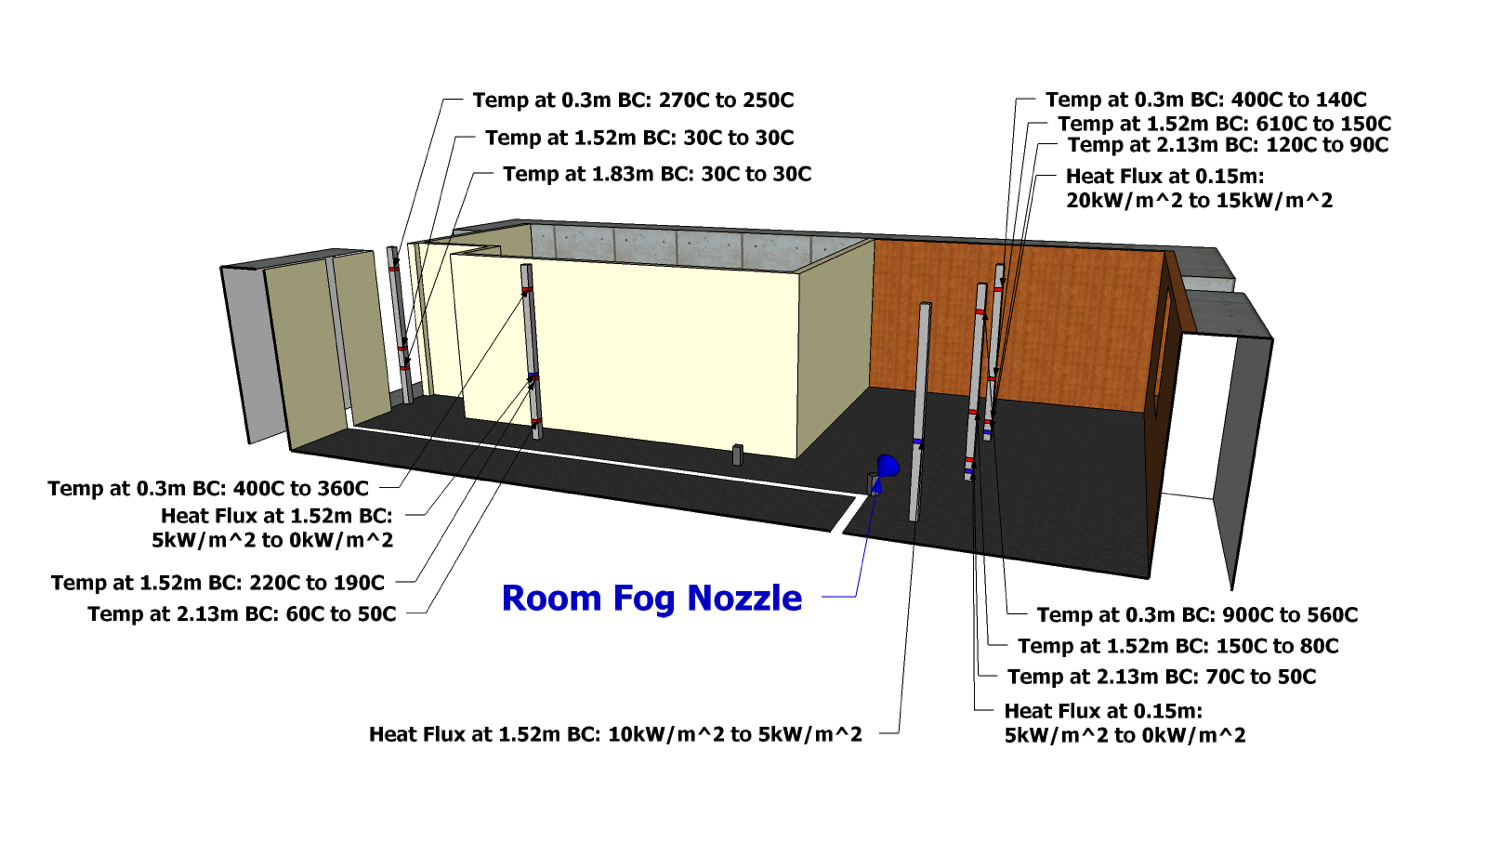
\includegraphics[width=6in]{../Figures/Pictures/Metric/DelCoFogTest11SecondSuppression}
	\caption{Test 11: Wood Fuel Package, Panel Window, Water, 30 deg Fog, 120 gpm, Second Suppression}
	\label{fig:Test_11_Second_Suppression}
\end{figure}

\begin{figure}[!ht]
	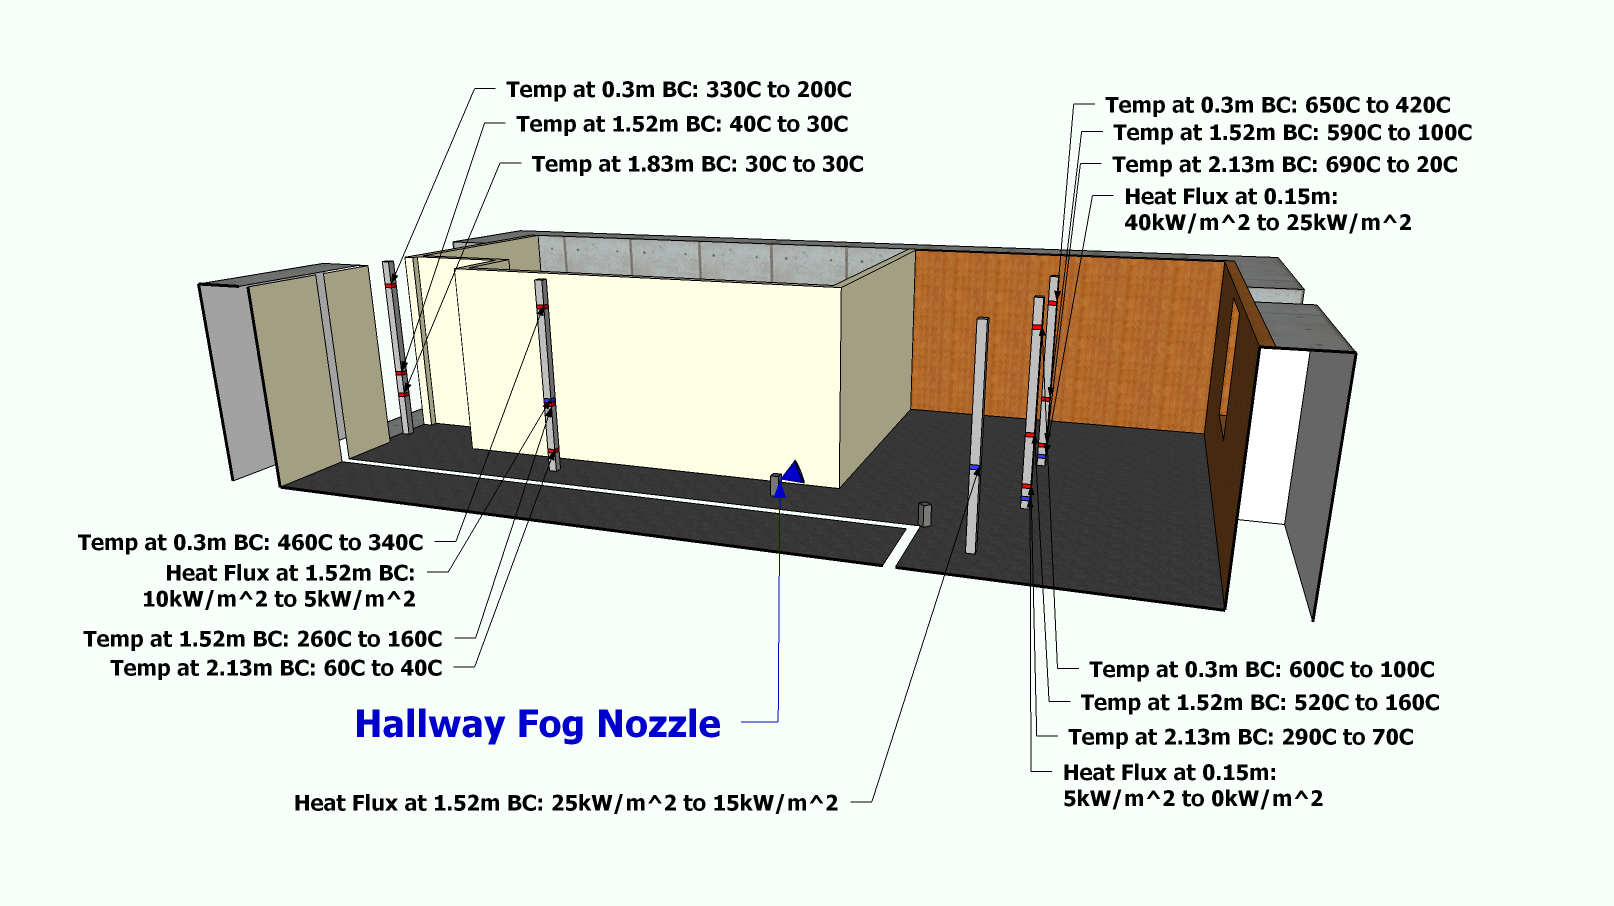
\includegraphics[width=6in]{../Figures/Pictures/Metric/DelCoFogTest12FirstSuppression}
	\caption{Test 12: Wood Fuel Package, Panel Window, CAFS, 30 deg Fog, 120 gpm/60cfm, First Suppression}
	\label{fig:Test_12_First_Suppression}
\end{figure}

\begin{figure}[!ht]
	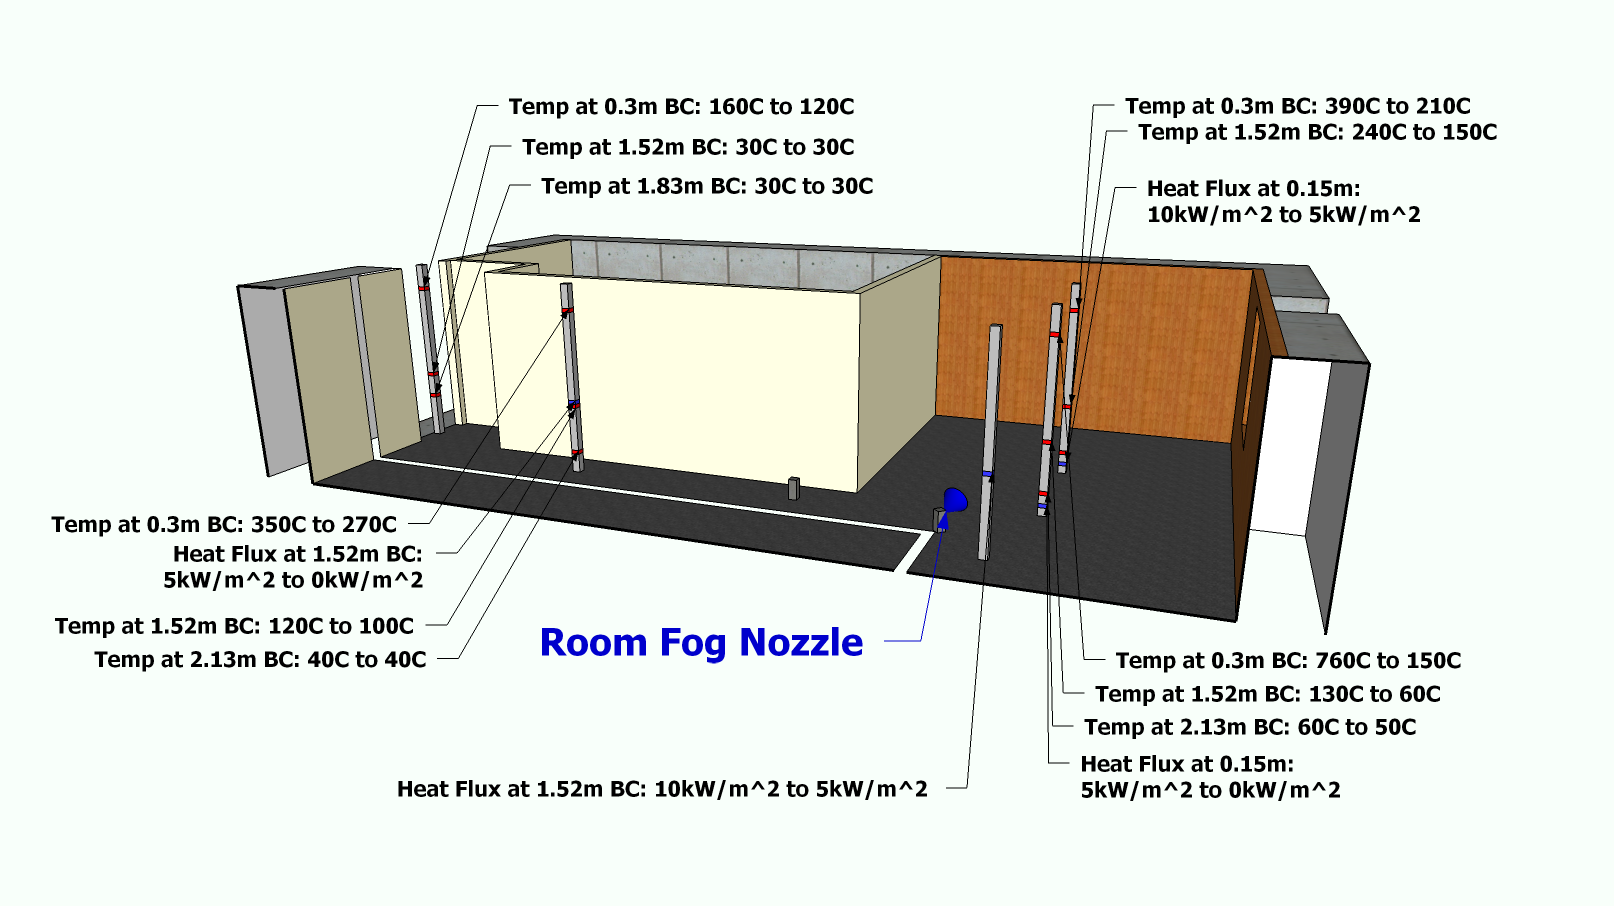
\includegraphics[width=6in]{../Figures/Pictures/Metric/DelCoFogTest12SecondSuppression}
	\caption{Test 12: Wood Fuel Package, Panel Window, CAFS, 30 deg Fog, 120 gpm/60cfm, Second Suppression}
	\label{fig:Test_12_Second_Suppression}
\end{figure}

\begin{figure}[!ht]
	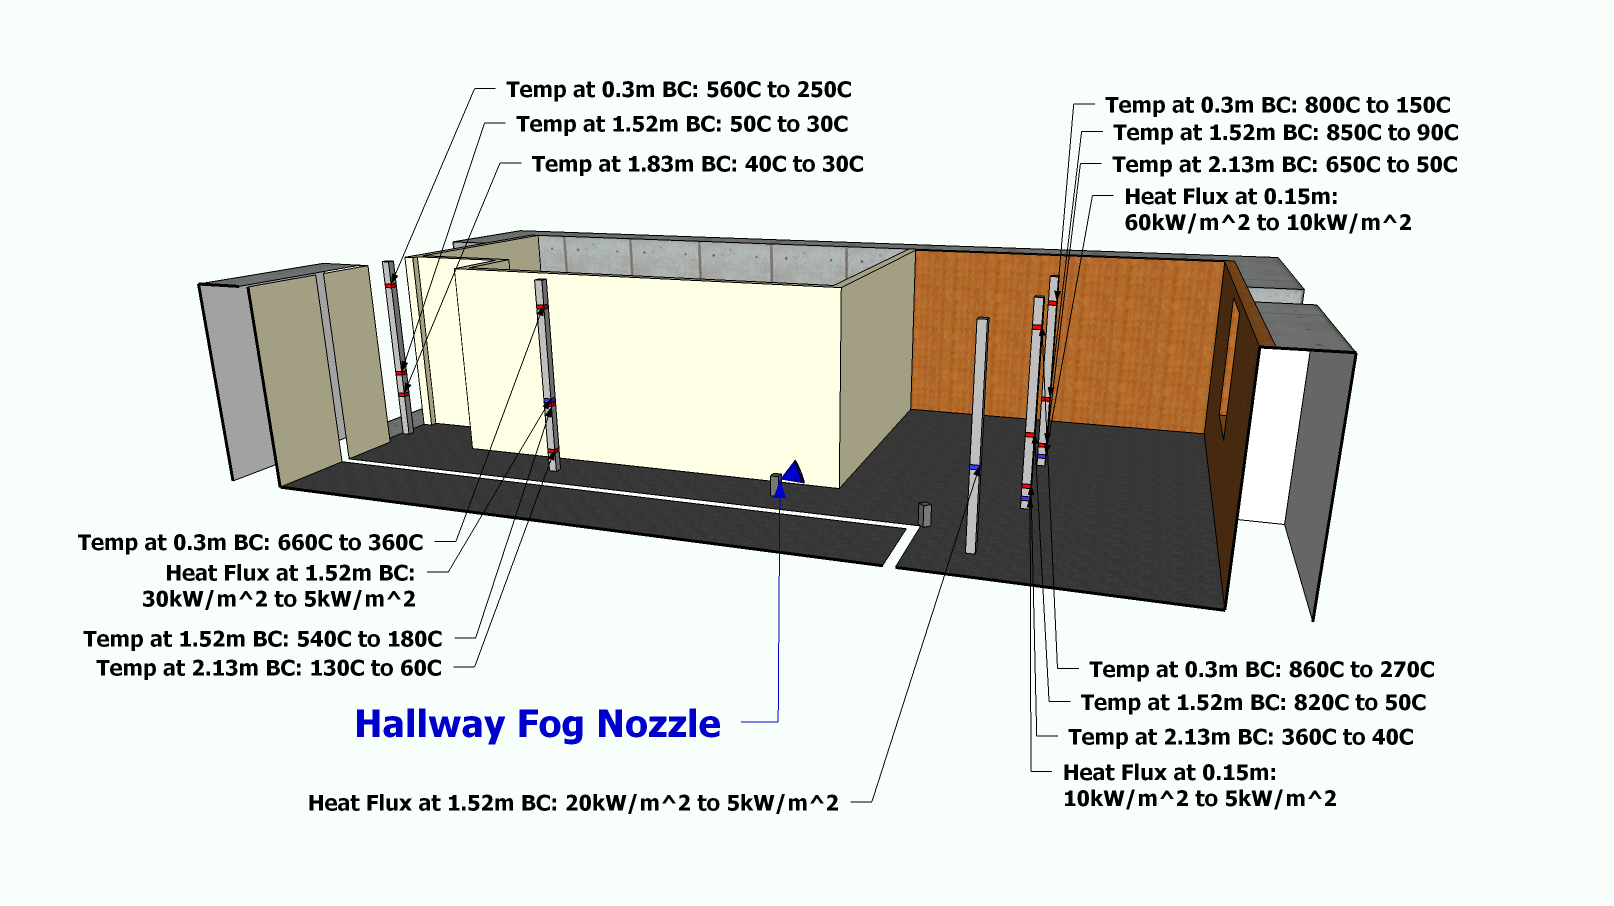
\includegraphics[width=6in]{../Figures/Pictures/Metric/DelCoFogTest13FirstSuppression}
	\caption{Test 13: Wood Fuel Package, Panel Window, Water, 30 deg Fog, 120 gpm, First Suppression}
	\label{fig:Test_13_First_Suppression}
\end{figure}

\begin{figure}[!ht]
	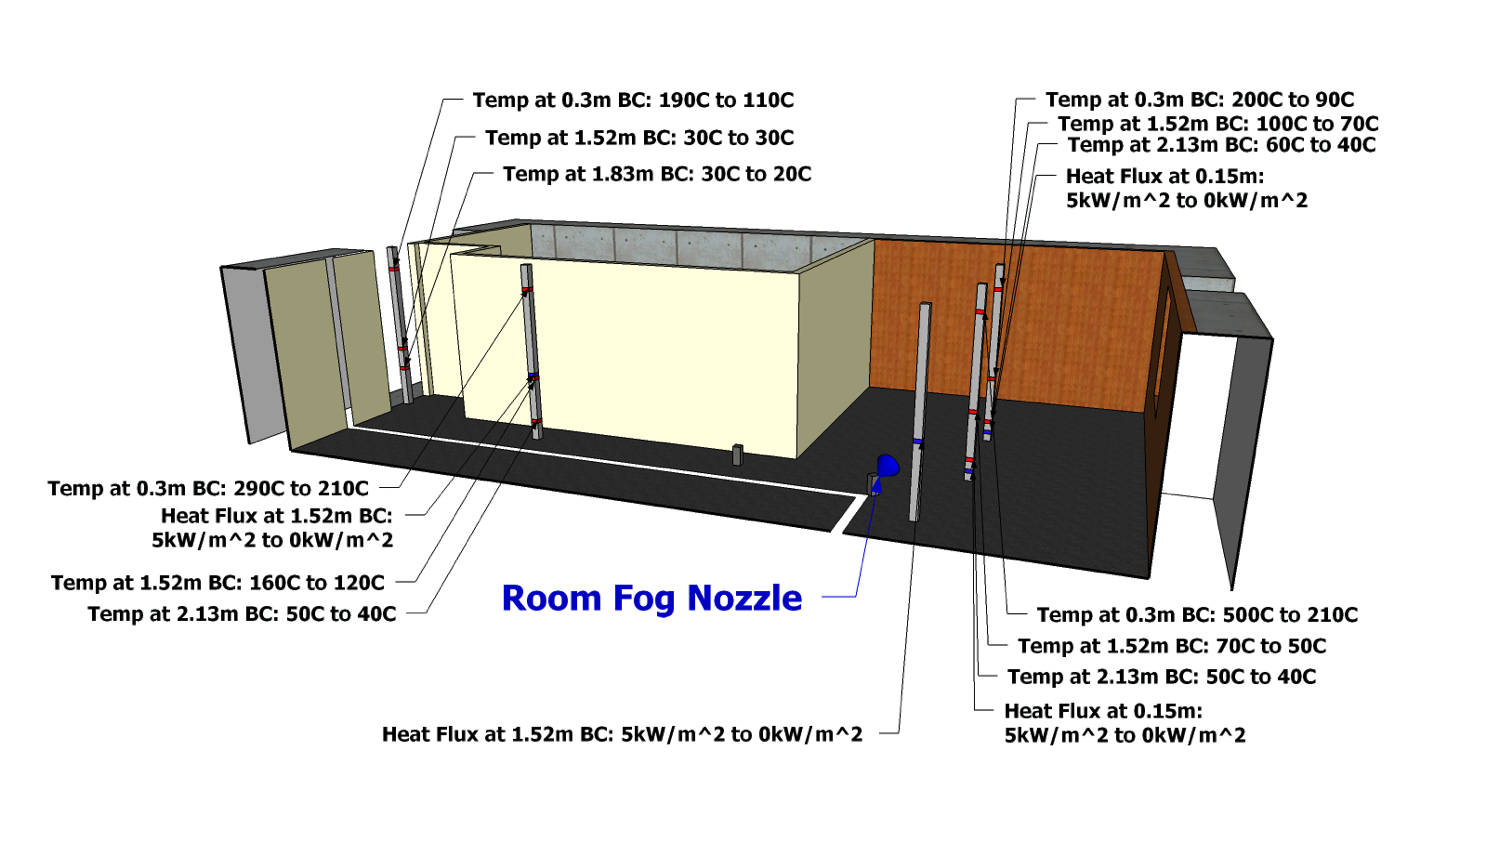
\includegraphics[width=6in]{../Figures/Pictures/Metric/DelCoFogTest13SecondSuppression}
	\caption{Test 13: Wood Fuel Package, Panel Window, Water, 30 deg Fog, 120 gpm, Second Suppression}
	\label{fig:Test_13_Second_Suppression}
\end{figure}

\begin{figure}[!ht]
	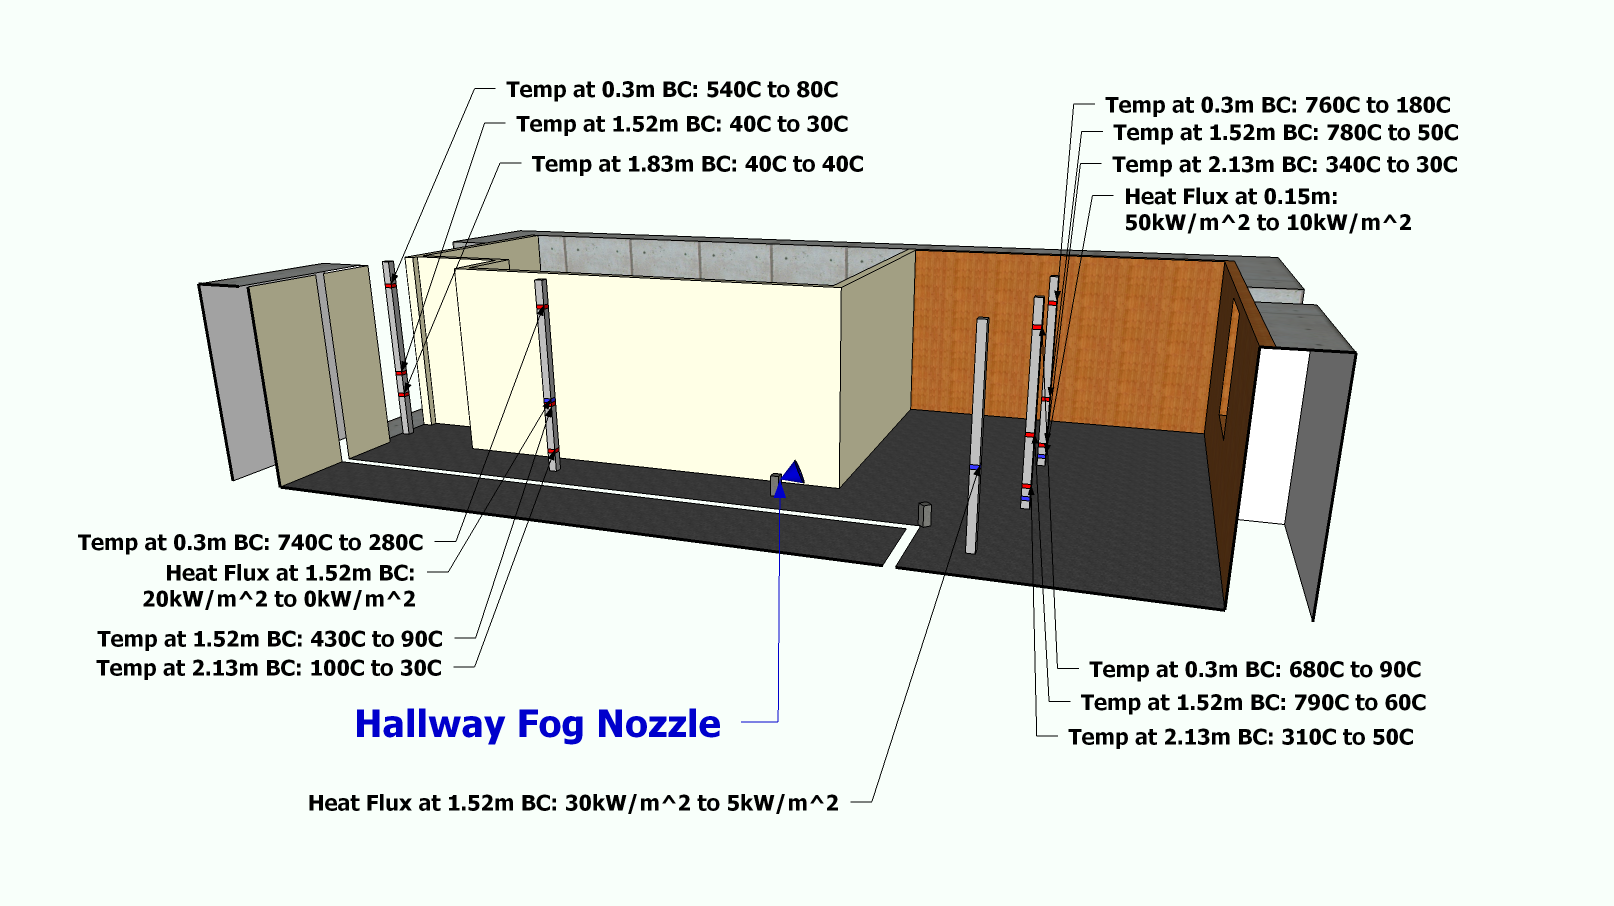
\includegraphics[width=6in]{../Figures/Pictures/Metric/DelCoFogTest14FirstSuppression}
	\caption{Test 14: Wood Fuel Package, Panel Window, CAFS, 30 deg Fog, 120 gpm/60cfm, First Suppression}
	\label{fig:Test_14_First_Suppression}
\end{figure}

\begin{figure}[!ht]
	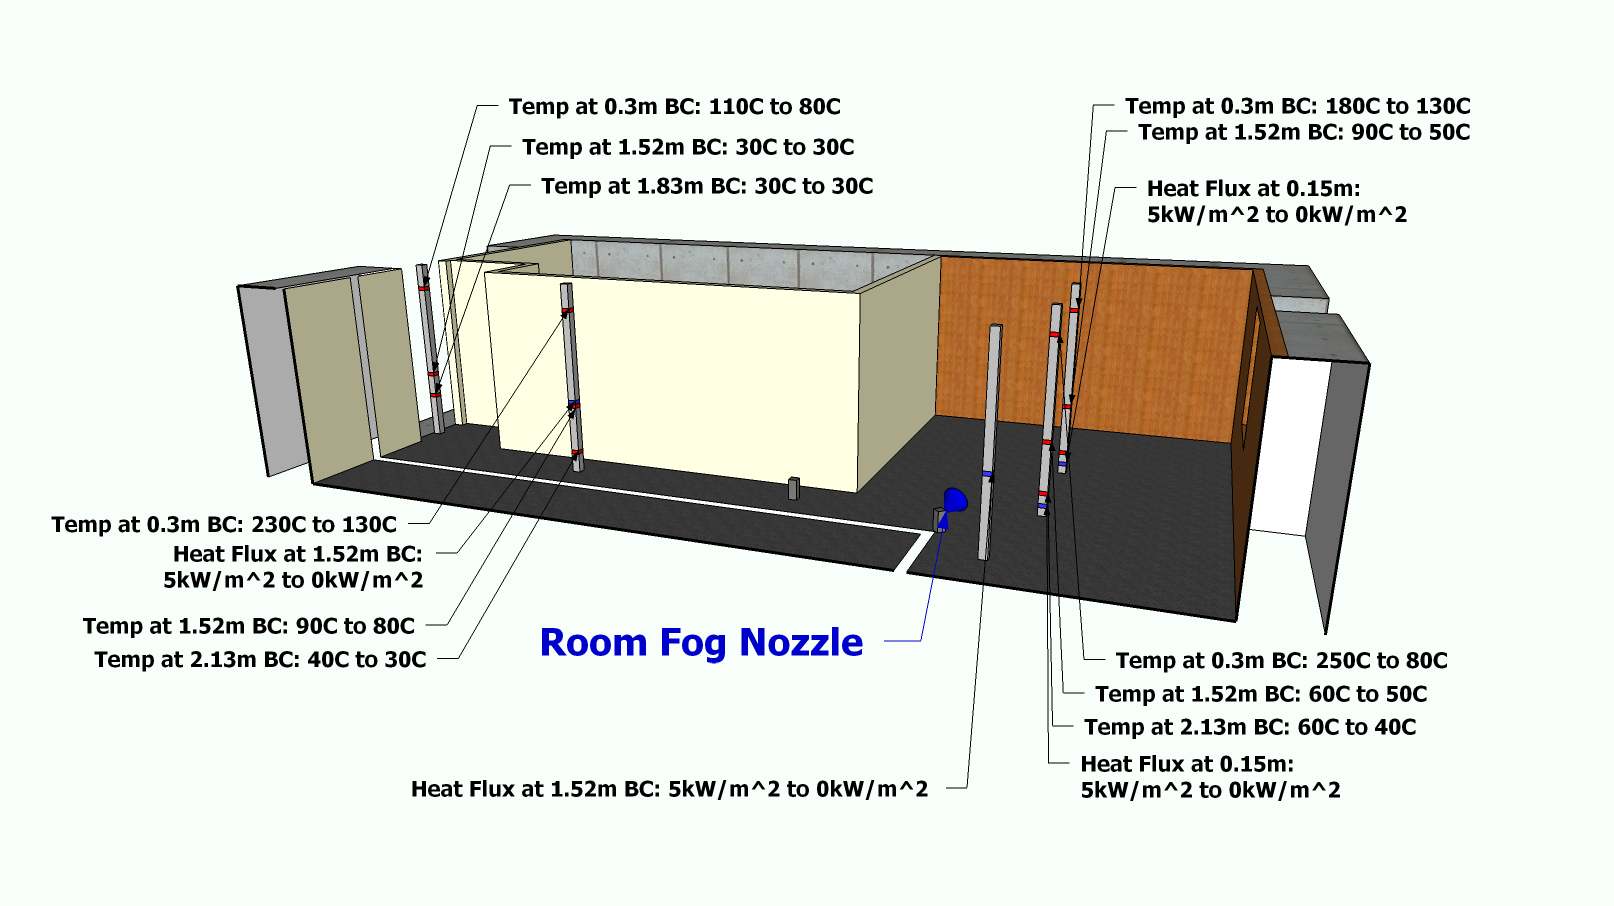
\includegraphics[width=6in]{../Figures/Pictures/Metric/DelCoFogTest14SecondSuppression}
	\caption{Test 14: Wood Fuel Package, Panel Window, CAFS, 30 deg Fog, 120 gpm/60cfm, Second Suppression}
	\label{fig:Test_14_Second_Suppression}
\end{figure}

\subsection{Furniture Fuel Package}
\label{subsec:Furniture_Fuel_Package}

\begin{figure}[!ht]
	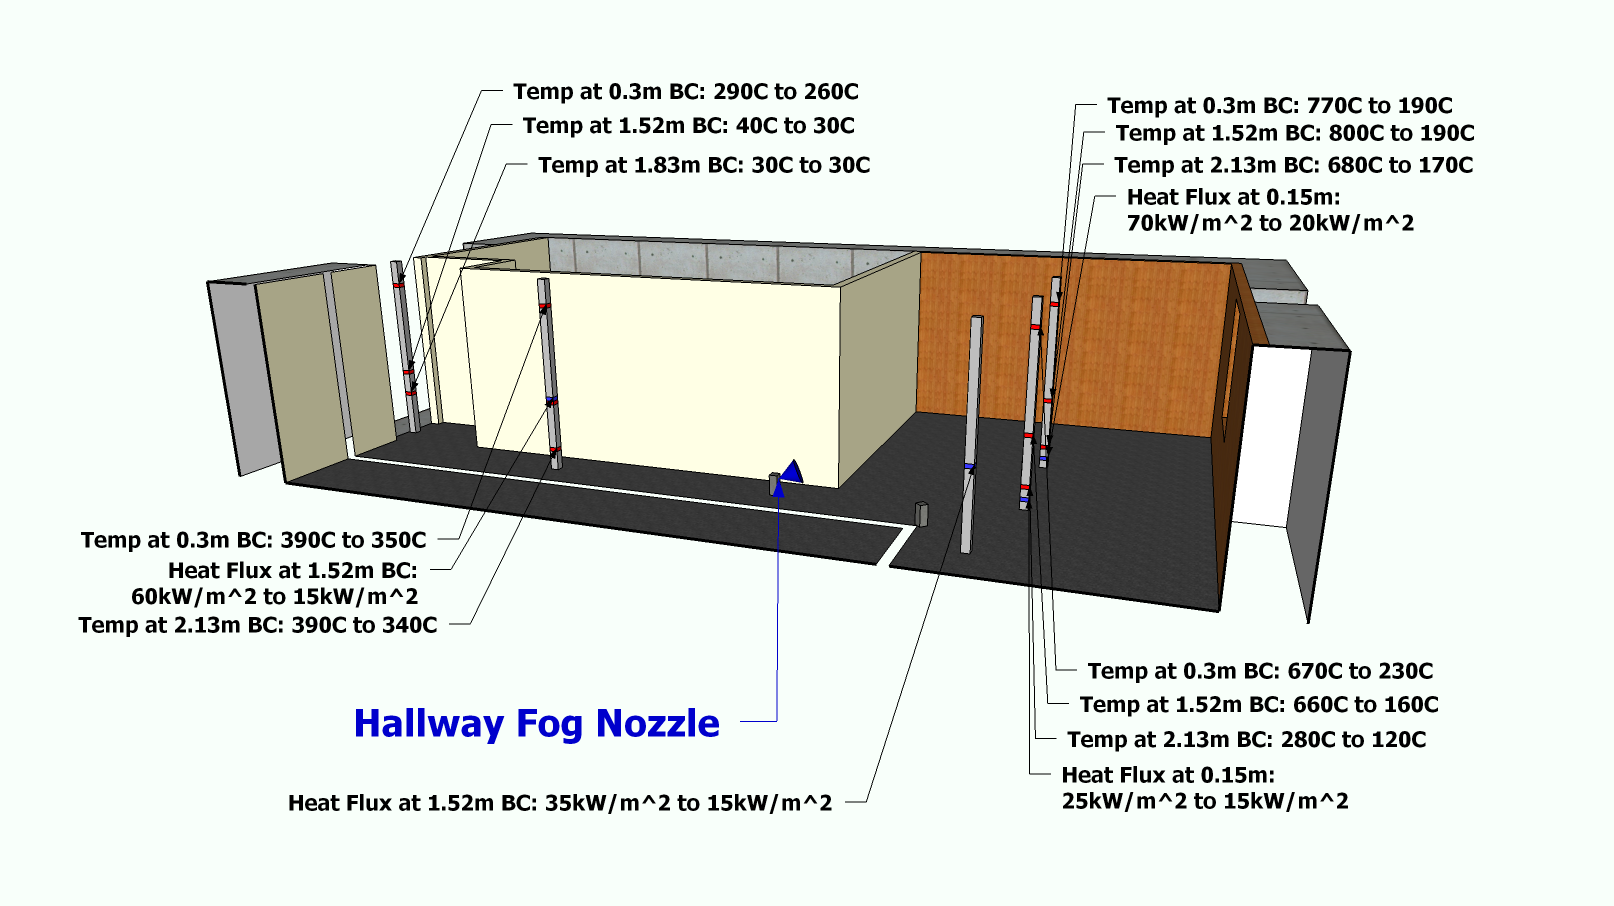
\includegraphics[width=6in]{../Figures/Pictures/Metric/DelCoFogTest1FirstSuppression}
	\caption{Test 1: Furniture Fuel Package, CAFS, 30 deg Fog, 120 gpm/60cfm, First Suppression}
	\label{fig:Test_1_First_Suppression}
\end{figure}

\begin{figure}[!ht]
	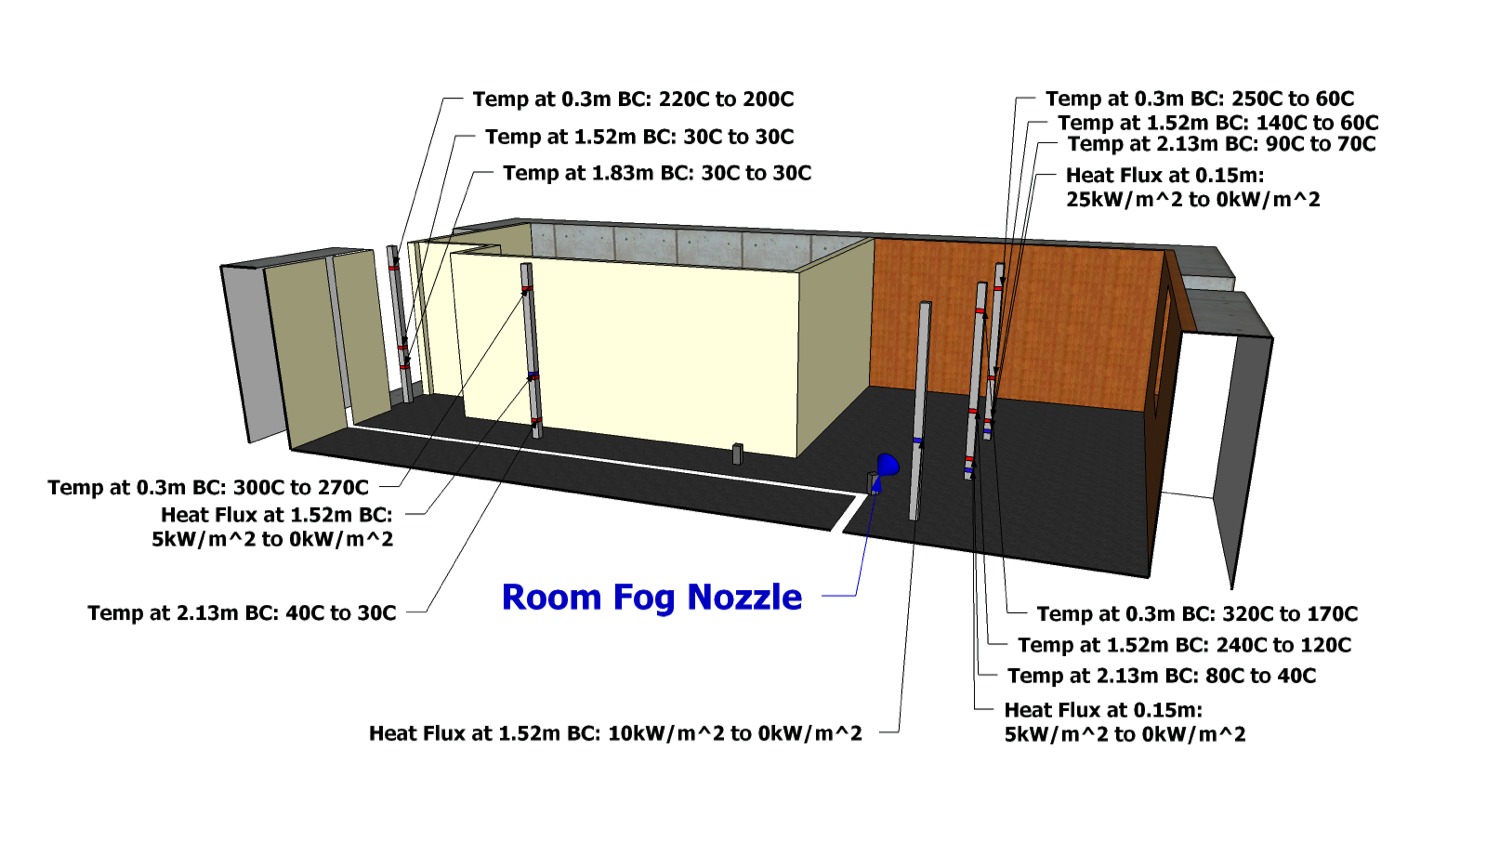
\includegraphics[width=6in]{../Figures/Pictures/Metric/DelCoFogTest1SecondSuppression}
	\caption{Test 1: Furniture Fuel Package, CAFS, 30 deg Fog, 120 gpm/60cfm, Second Suppression}
	\label{fig:Test_1_Second_Suppression}
\end{figure}

\begin{figure}[!ht]
	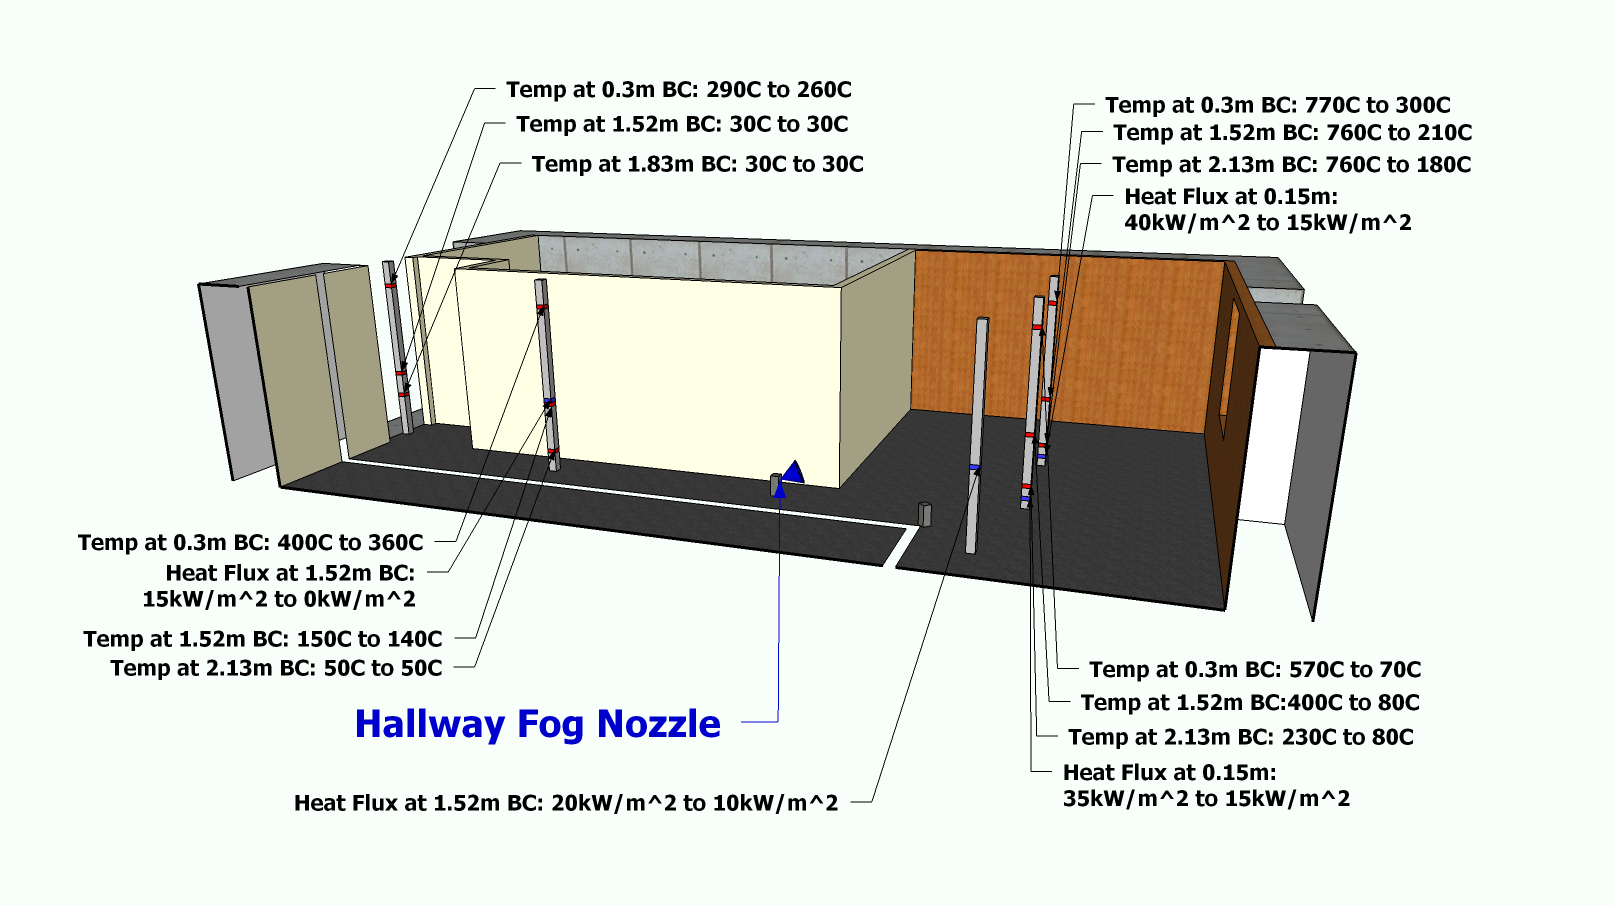
\includegraphics[width=6in]{../Figures/Pictures/Metric/DelCoFogTest2FirstSuppression}
	\caption{Test 2: Furniture Fuel Package, Water, 30 deg Fog, 120 gpm, First Suppression}
	\label{fig:Test_2_First_Suppression}
\end{figure}

\begin{figure}[!ht]
	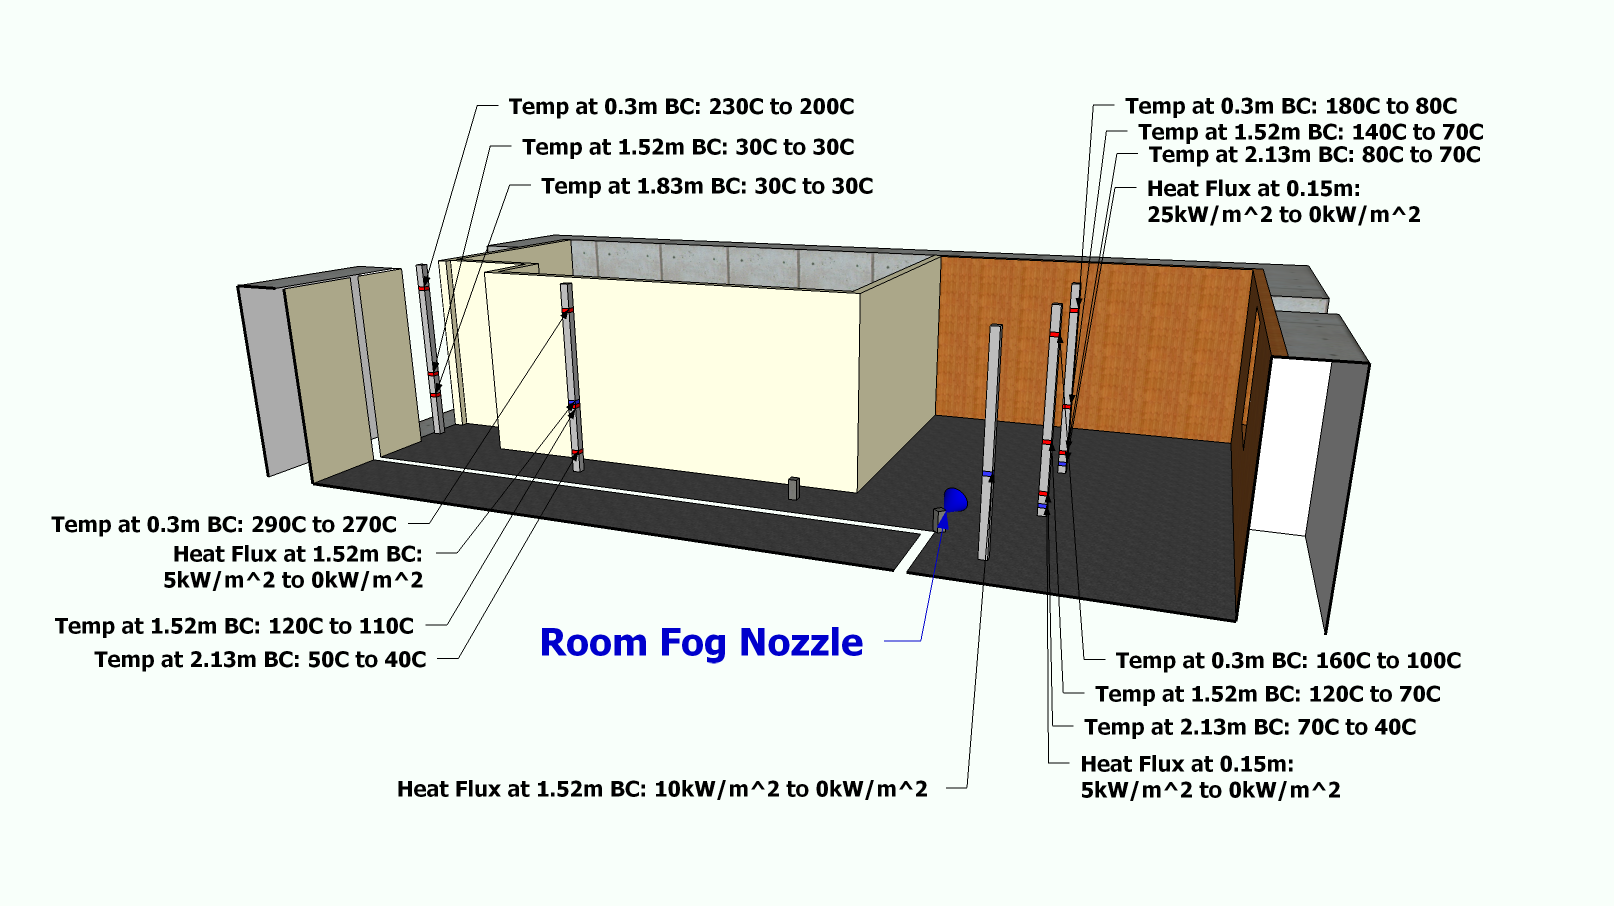
\includegraphics[width=6in]{../Figures/Pictures/Metric/DelCoFogTest2SecondSuppression}
	\caption{Test 2: Furniture Fuel Package, Water, 30 deg Fog, 120 gpm, Second Suppression}
	\label{fig:Test_2_Second_Suppression}
\end{figure}

\begin{figure}[!ht]
	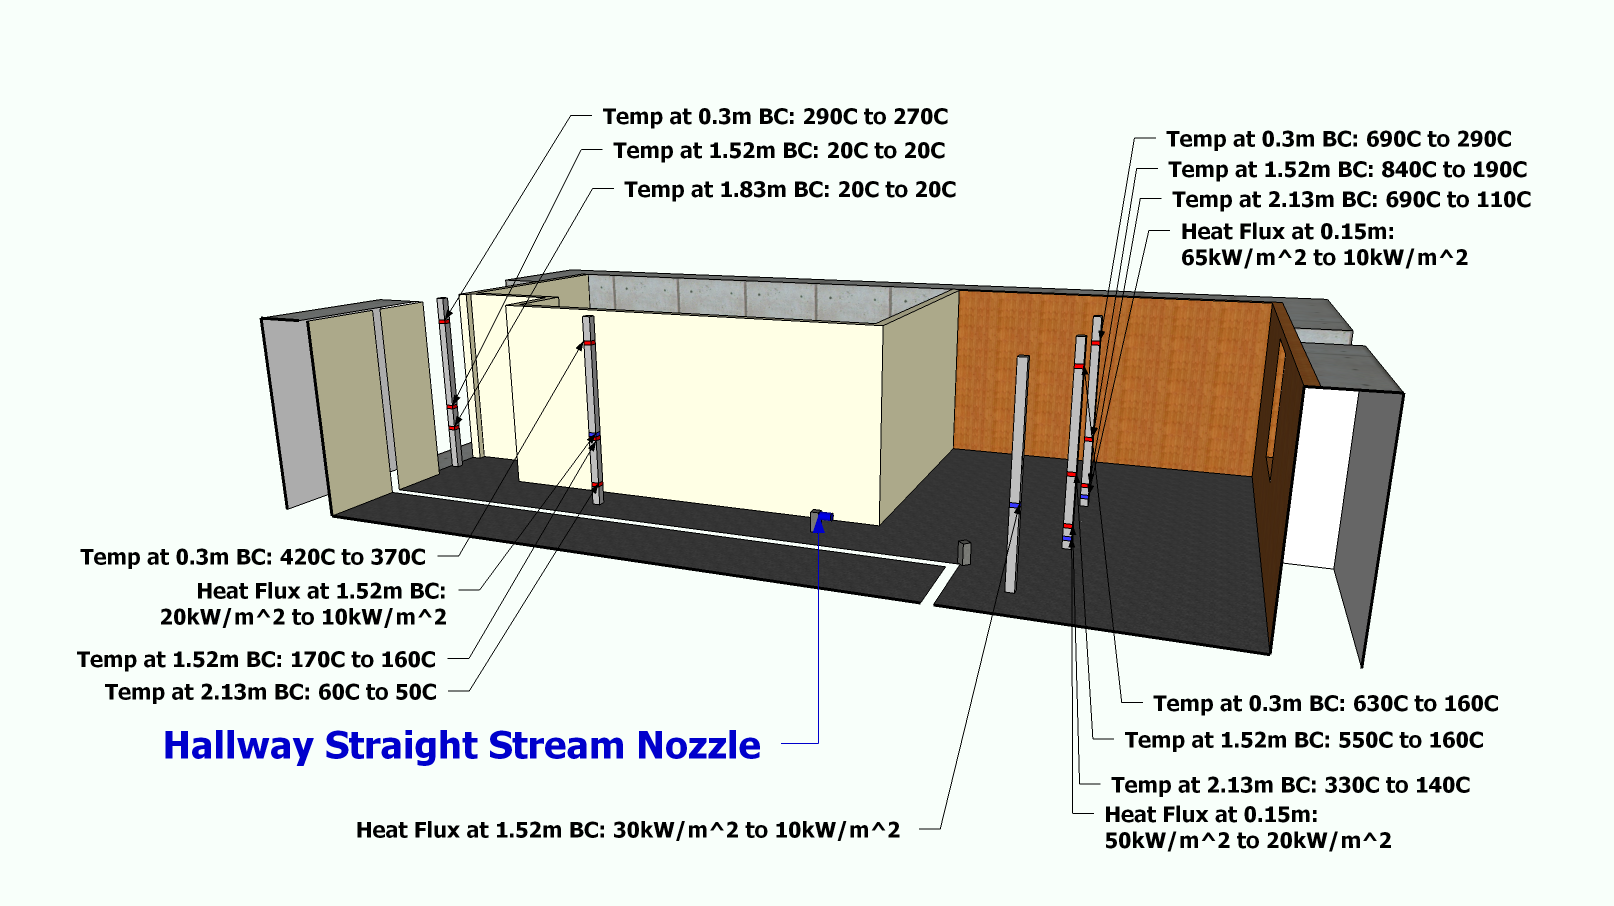
\includegraphics[width=6in]{../Figures/Pictures/Metric/DelCoSSTest3FirstSuppression}
	\caption{Test 3: Furniture Fuel Package, CAFS, 7/8" Smooth Bore, 120 gpm/60 cfm, First Suppression}
	\label{fig:Test_3_First_Suppression}
\end{figure}

\begin{figure}[!ht]
	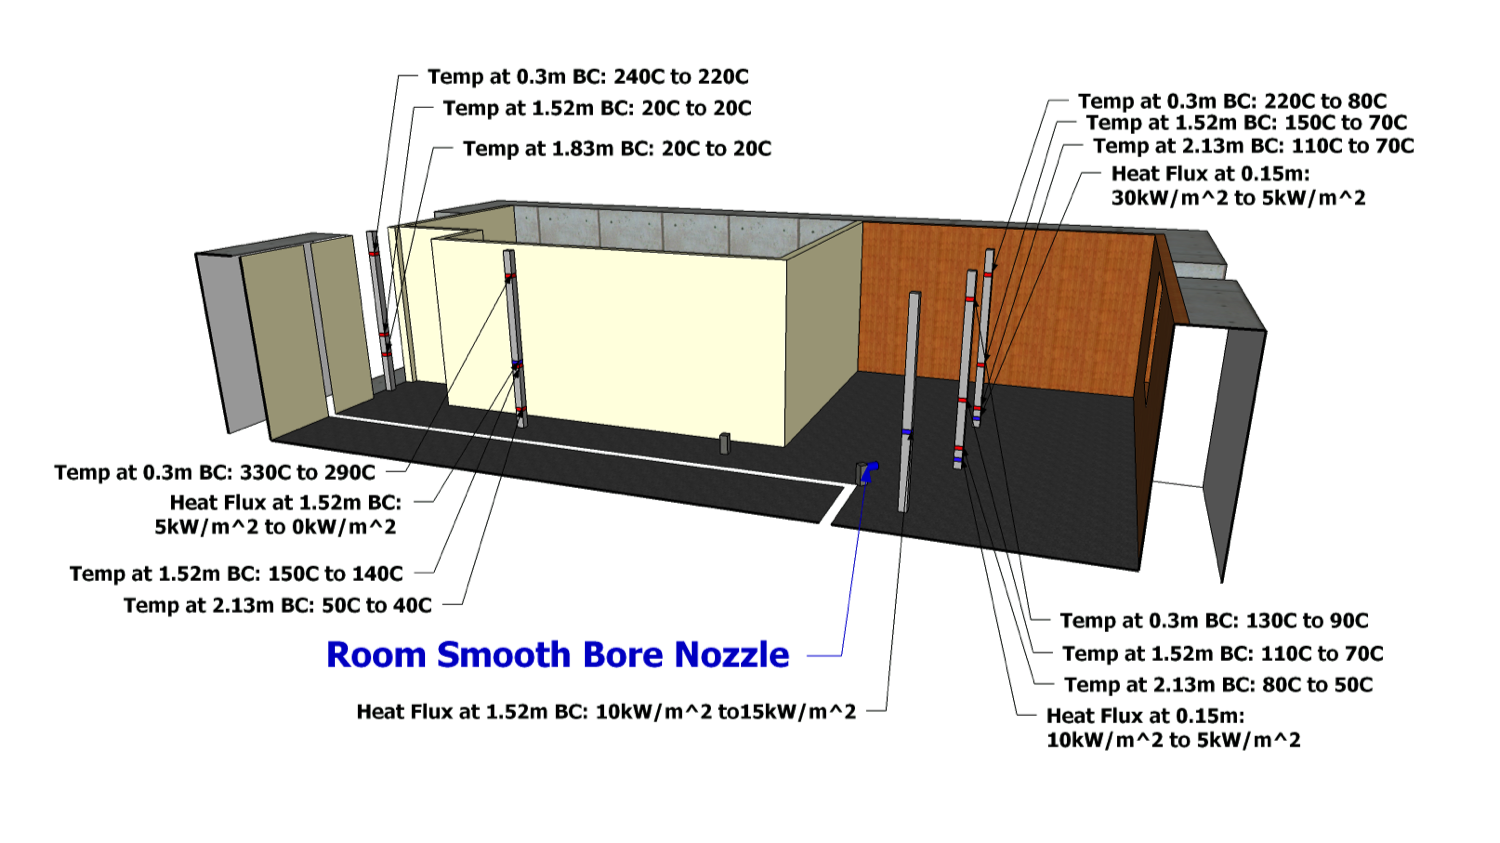
\includegraphics[width=6in]{../Figures/Pictures/Metric/DelCoSSTest3SecondSuppression}
	\caption{Test 3: Furniture Fuel Package, CAFS, 7/8" Smooth Bore, 120 gpm/60 cfm, Second Suppression}
	\label{fig:Test_3_Second_Suppression}
\end{figure}

\begin{figure}[!ht]
	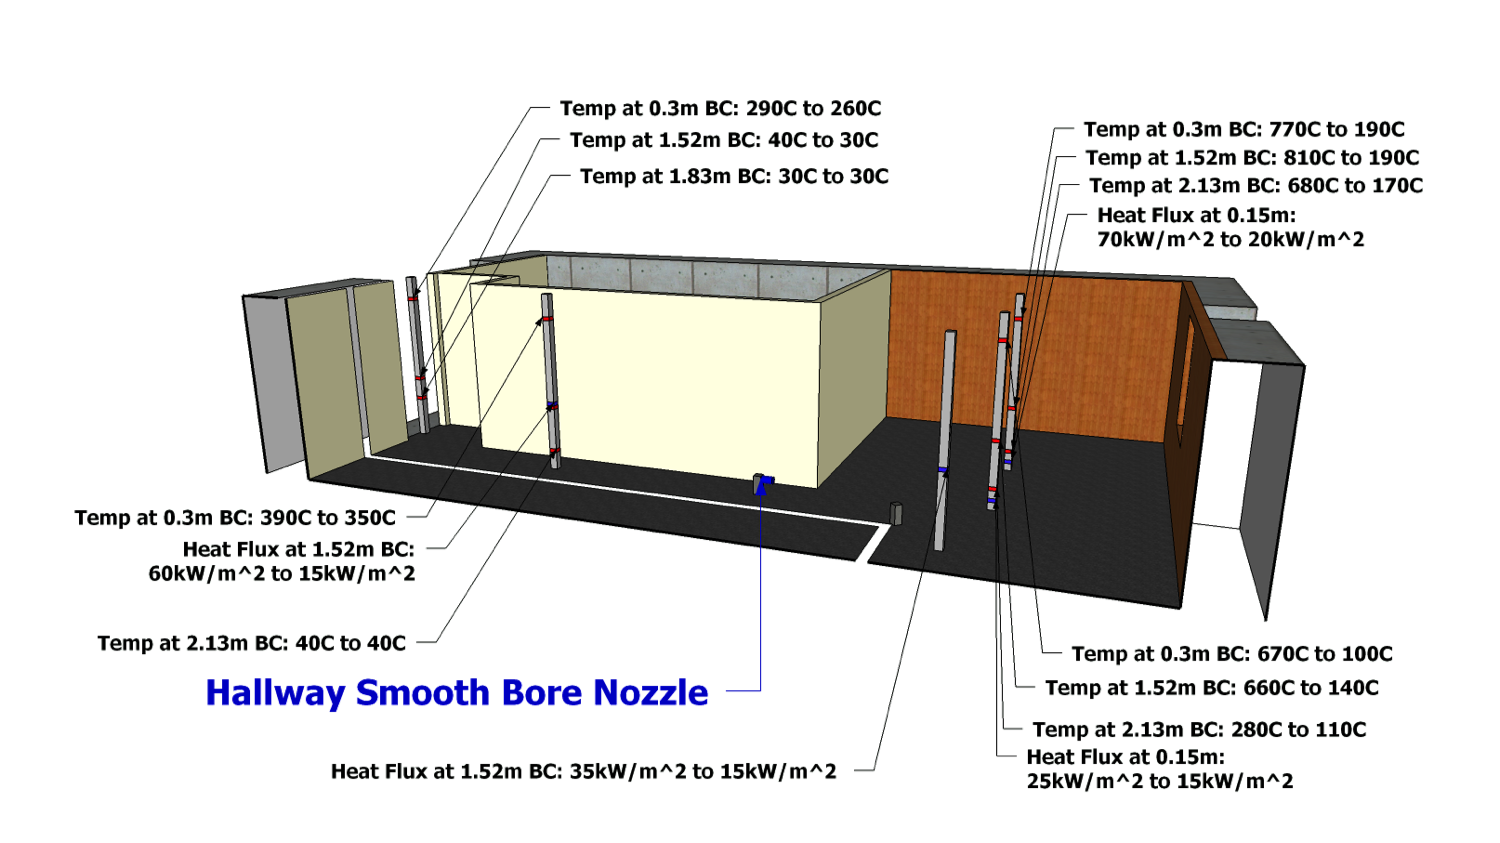
\includegraphics[width=6in]{../Figures/Pictures/Metric/DelCoSSTest4FirstSuppression}
	\caption{Test 4: Furniture Fuel Package, Water, 7/8" Smooth Bore, 120 gpm, First Suppression}
	\label{fig:Test_4_First_Suppression}
\end{figure}

\begin{figure}[!ht]
	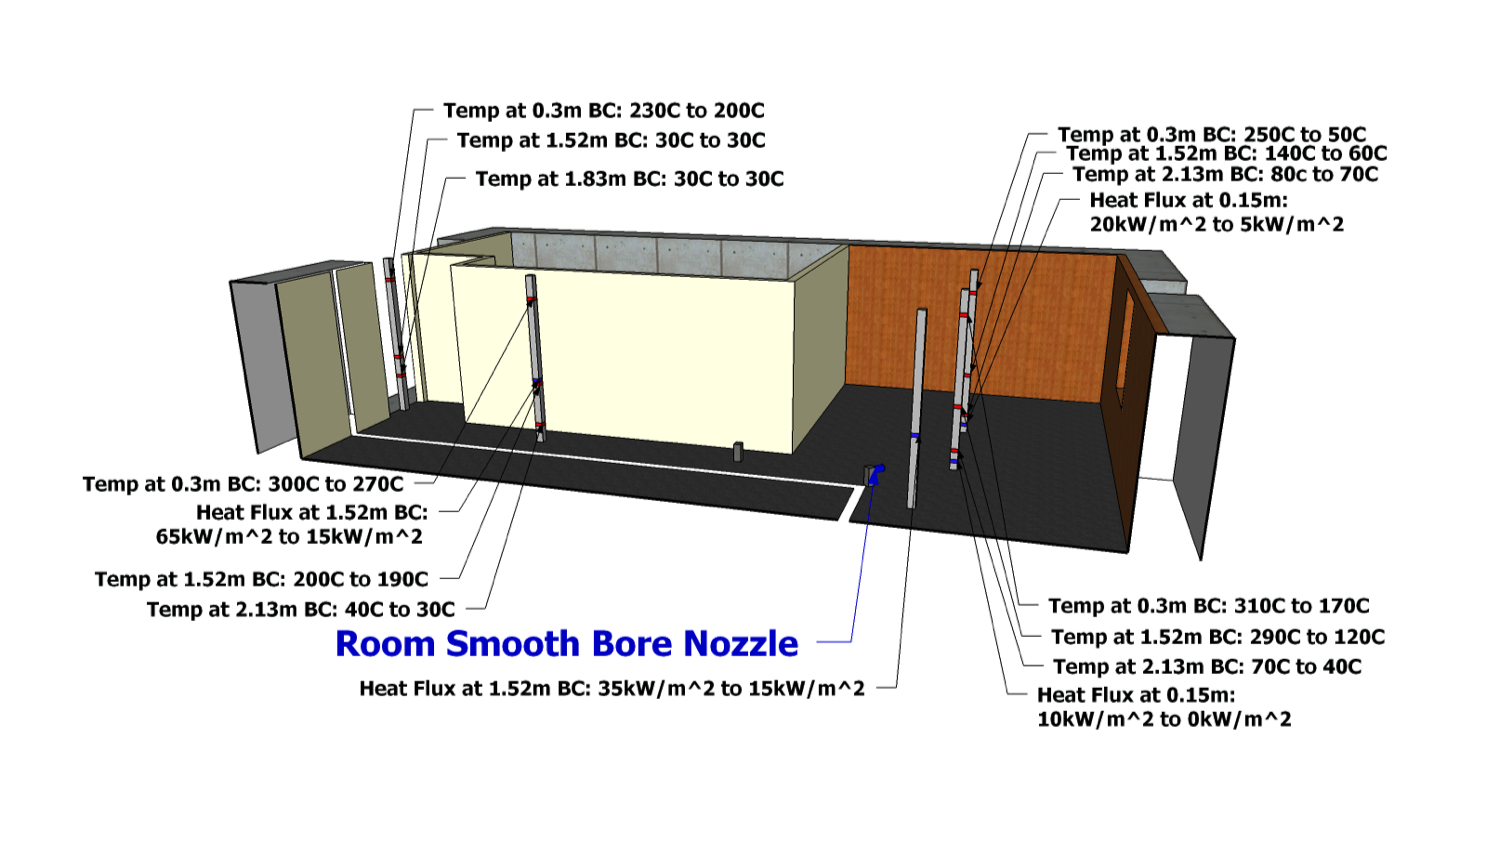
\includegraphics[width=6in]{../Figures/Pictures/Metric/DelCoSSTest4SecondSuppression}
	\caption{Test 4: Furniture Fuel Package, Water, 7/8" Smooth Bore, 120 gpm, Second Suppression}
	\label{fig:Test_4_Second_Suppression}
\end{figure}

\begin{figure}[!ht]
	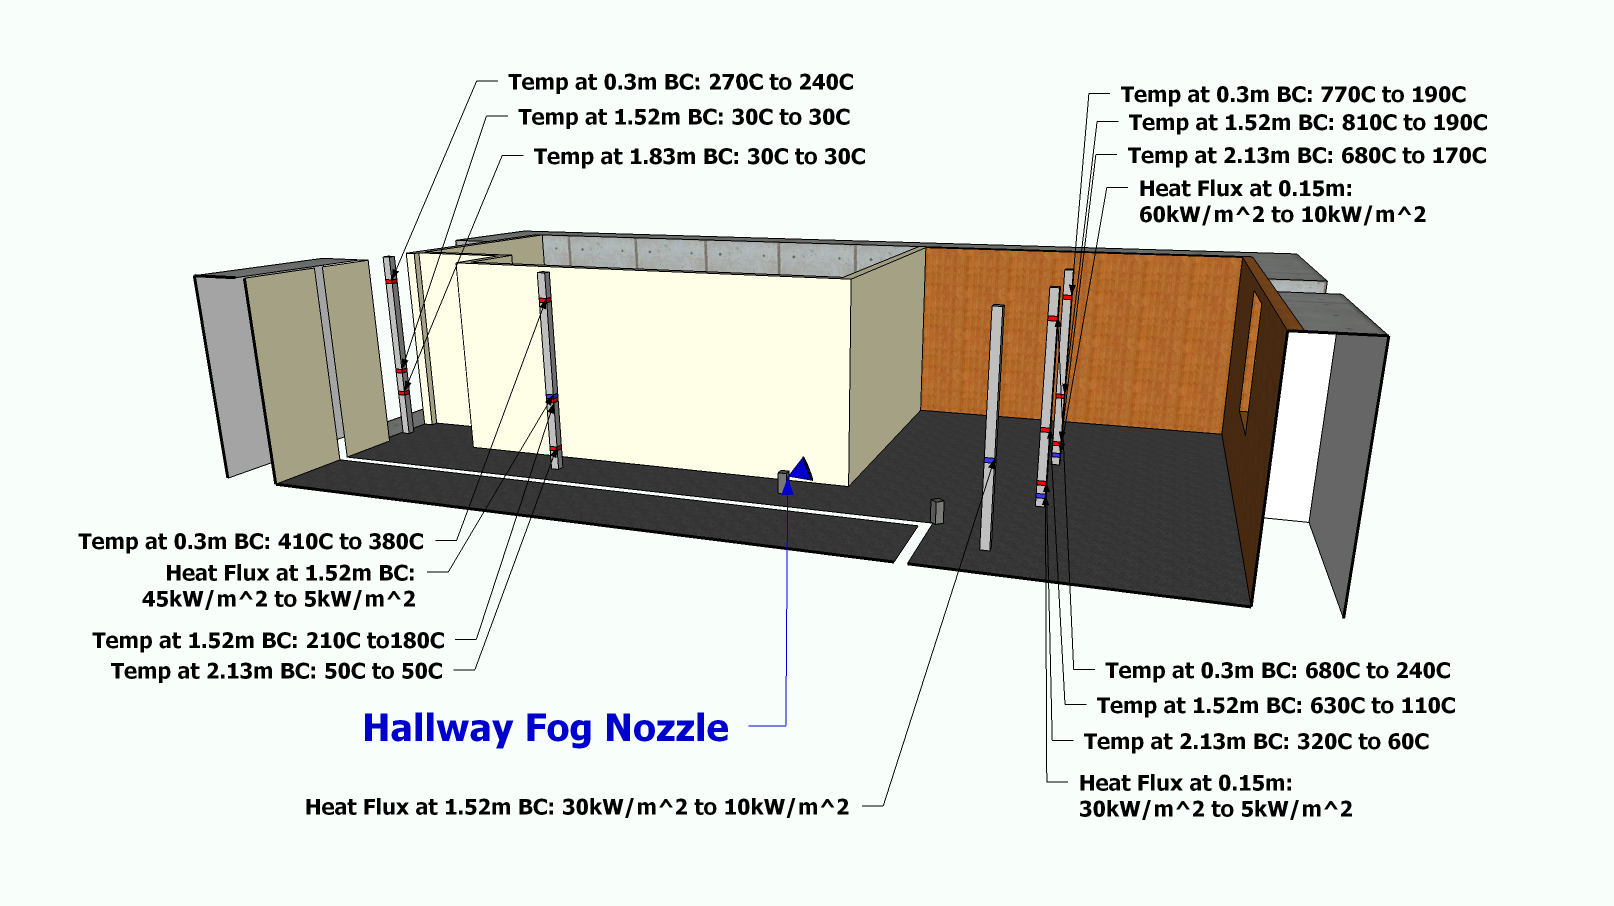
\includegraphics[width=6in]{../Figures/Pictures/Metric/DelCoFogTest5FirstSuppression}
	\caption{Test 5: Furniture Fuel Package, Water, 30 deg Fog, 120 gpm, First Suppression}
	\label{fig:Test_5_First_Suppression}
\end{figure}

\begin{figure}[!ht]
	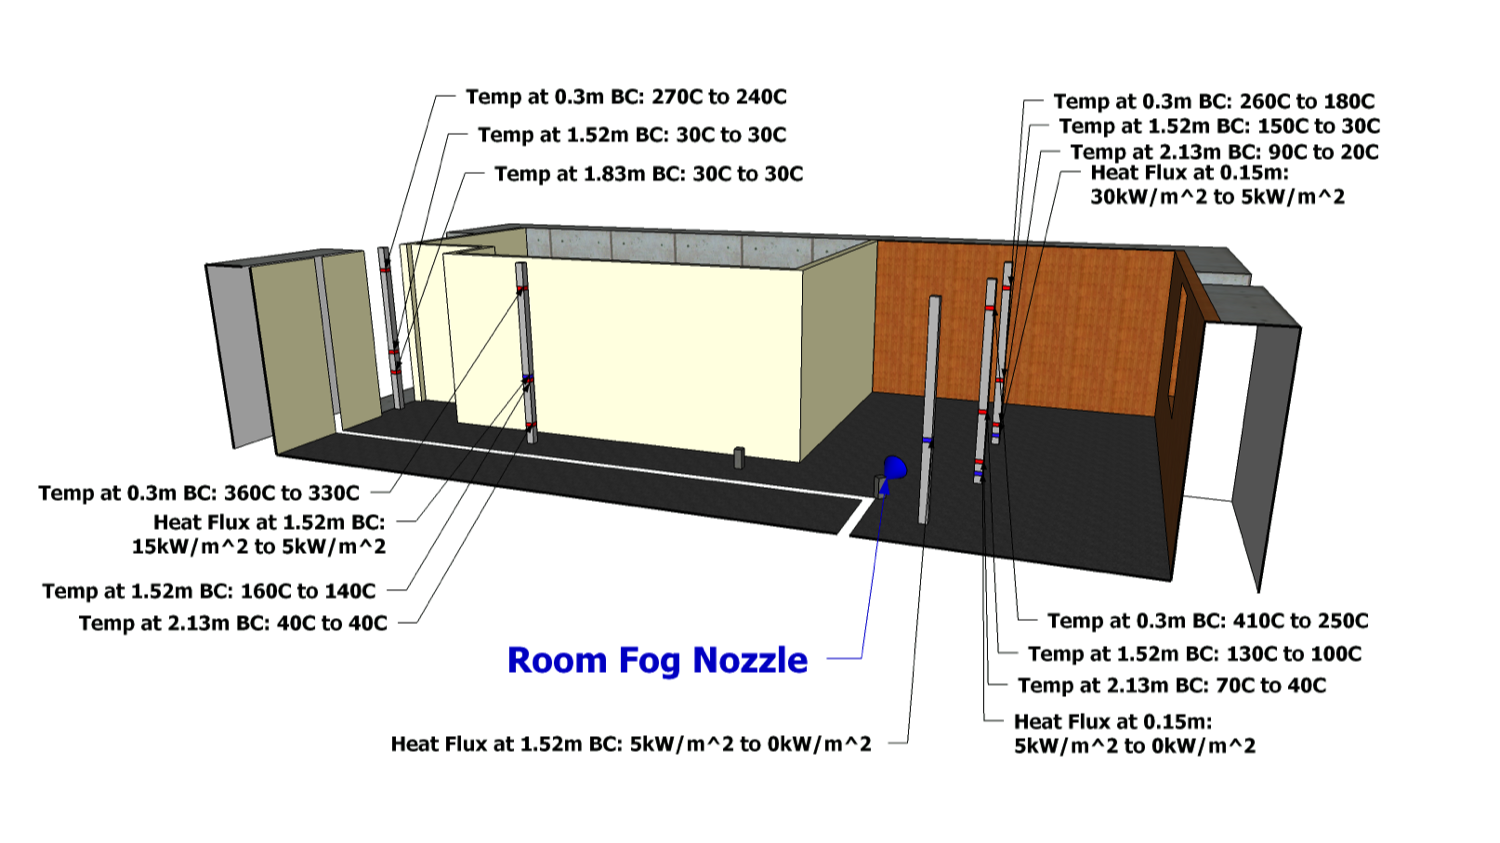
\includegraphics[width=6in]{../Figures/Pictures/Metric/DelCoFogTest5SecondSuppression}
	\caption{Test 5: Furniture Fuel Package, Water, 30 deg Fog, 120 gpm, Second Suppression}
	\label{fig:Test_5_Second_Suppression}
\end{figure}

\begin{figure}[!ht]
	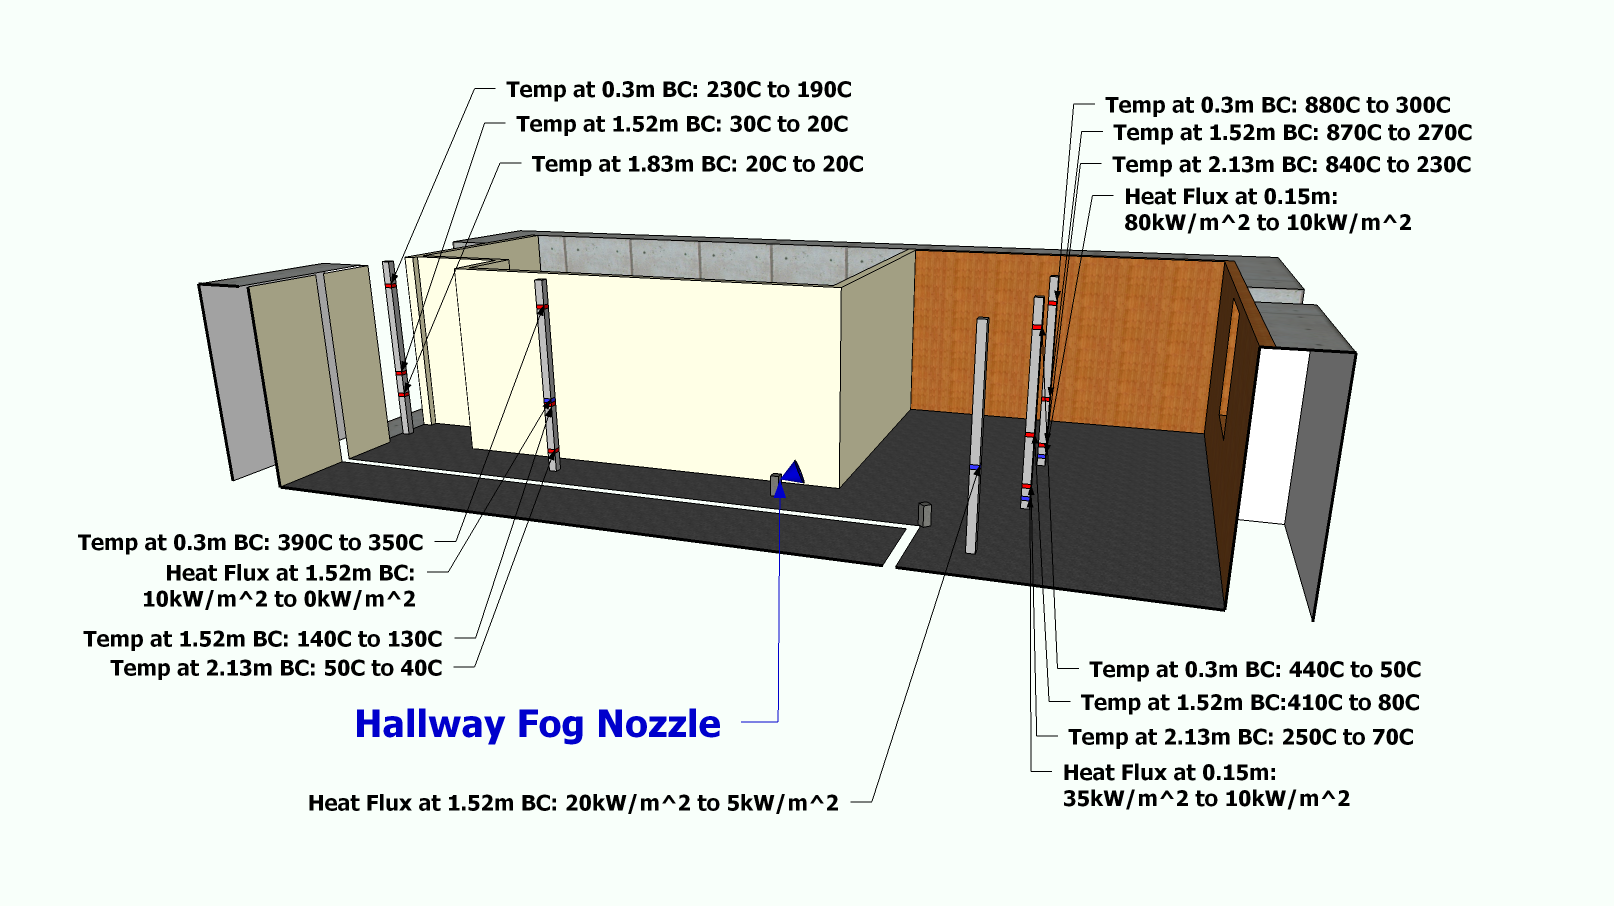
\includegraphics[width=6in]{../Figures/Pictures/Metric/DelCoFogTest6FirstSuppression}
	\caption{Test 6: Furniture Fuel Package, CAFS, 30 deg Fog, 120 gpm/60cfm, First Suppression}
	\label{fig:Test_6_First_Suppression}
\end{figure}

\begin{figure}[!ht]
	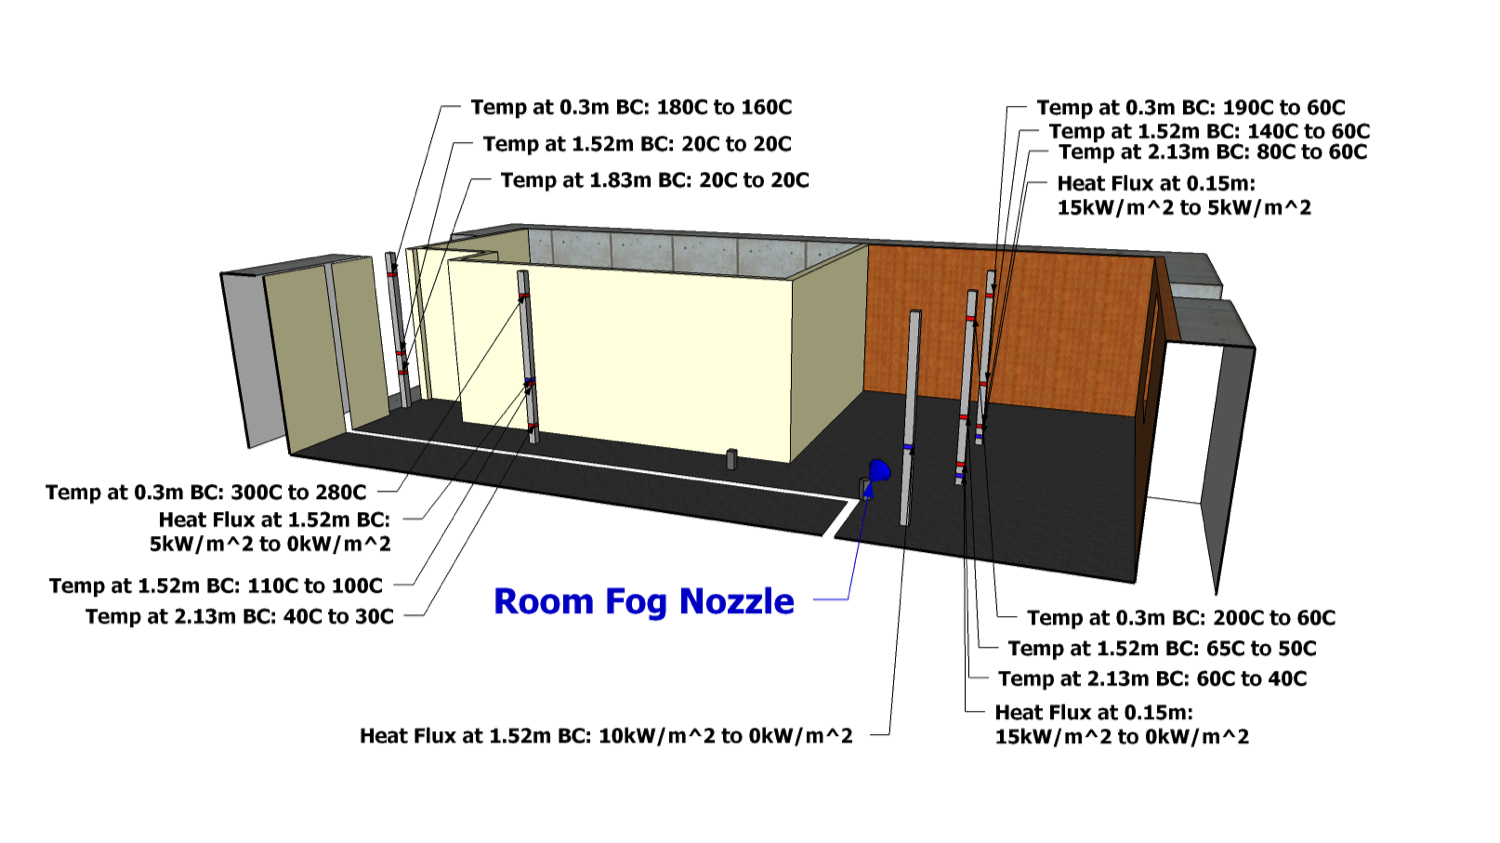
\includegraphics[width=6in]{../Figures/Pictures/Metric/DelCoFogTest6SecondSuppression}
	\caption{Test 6: Furniture Fuel Package, CAFS, 30 deg Fog, 120 gpm/60cfm, Second Suppression}
	\label{fig:Test_6_Second_Suppression}
\end{figure}

\begin{figure}[!ht]
	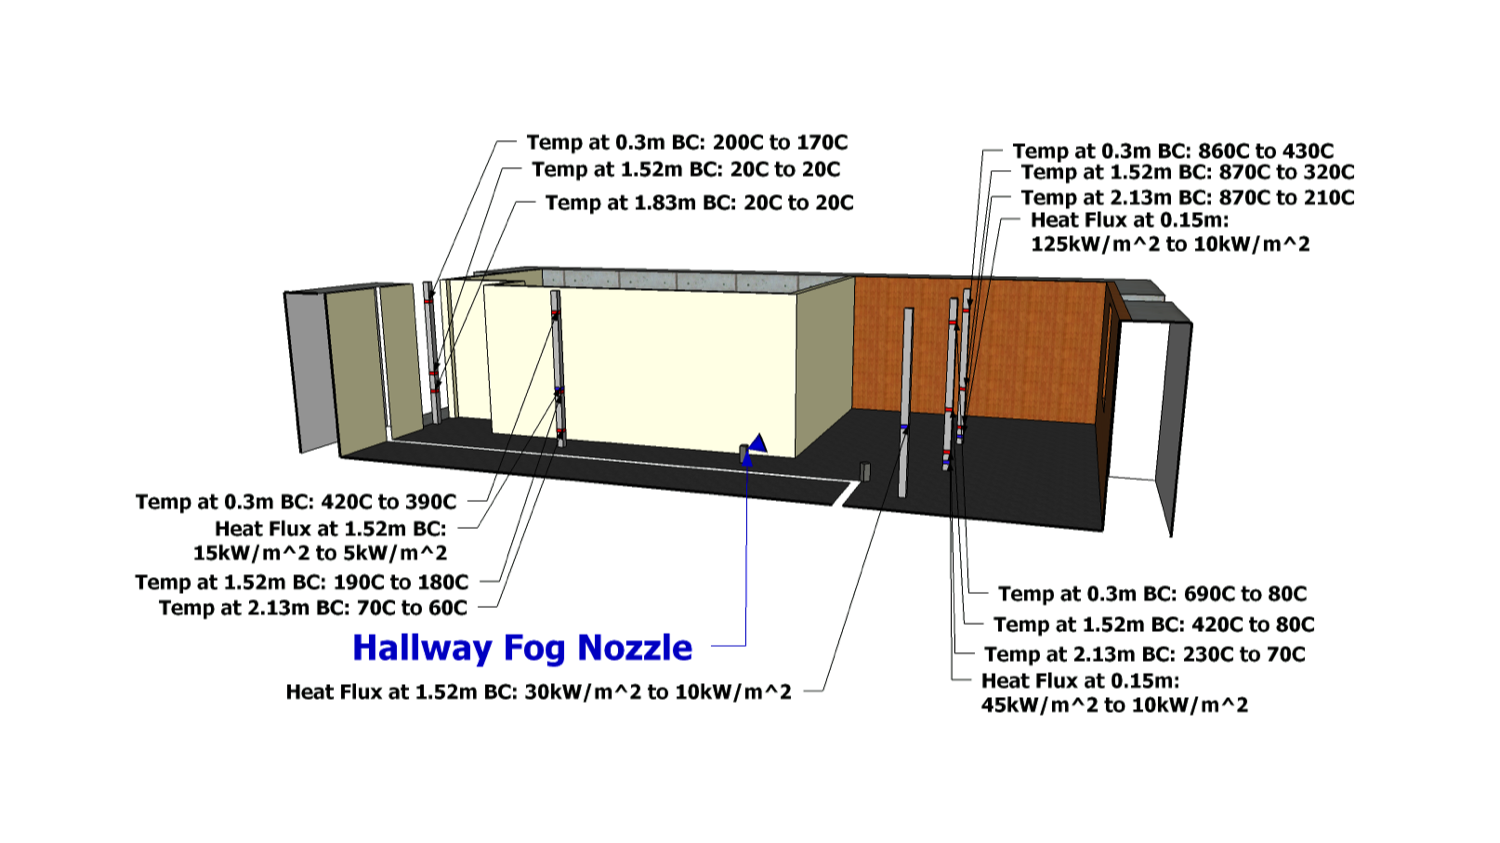
\includegraphics[width=6in]{../Figures/Pictures/Metric/DelCoFogTest7FirstSuppression}
	\caption{Test 7: Furniture Fuel Package, Water, 30 deg Fog, 120 gpm, First Suppression}
	\label{fig:Test_7_First_Suppression}
\end{figure}

\begin{figure}[!ht]
	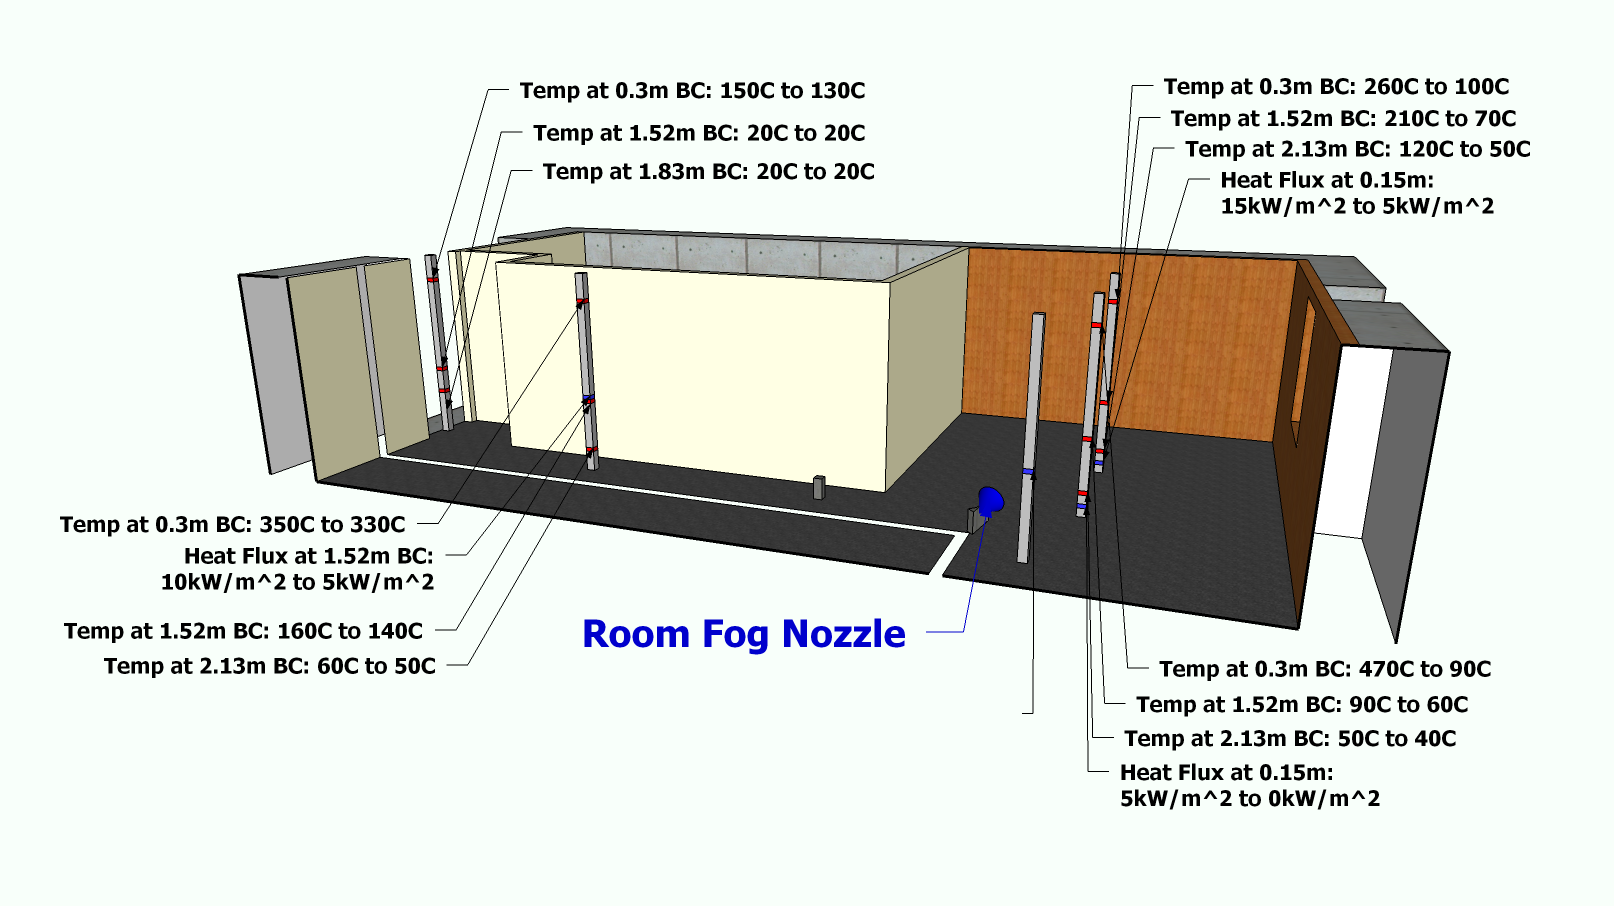
\includegraphics[width=6in]{../Figures/Pictures/Metric/DelCoFogTest7SecondSuppression}
	\caption{Test 7: Furniture Fuel Package, Water, 30 deg Fog, 120 gpm, Second Suppression}
	\label{fig:Test_7_Second_Suppression}
\end{figure}

\begin{figure}[!ht]
	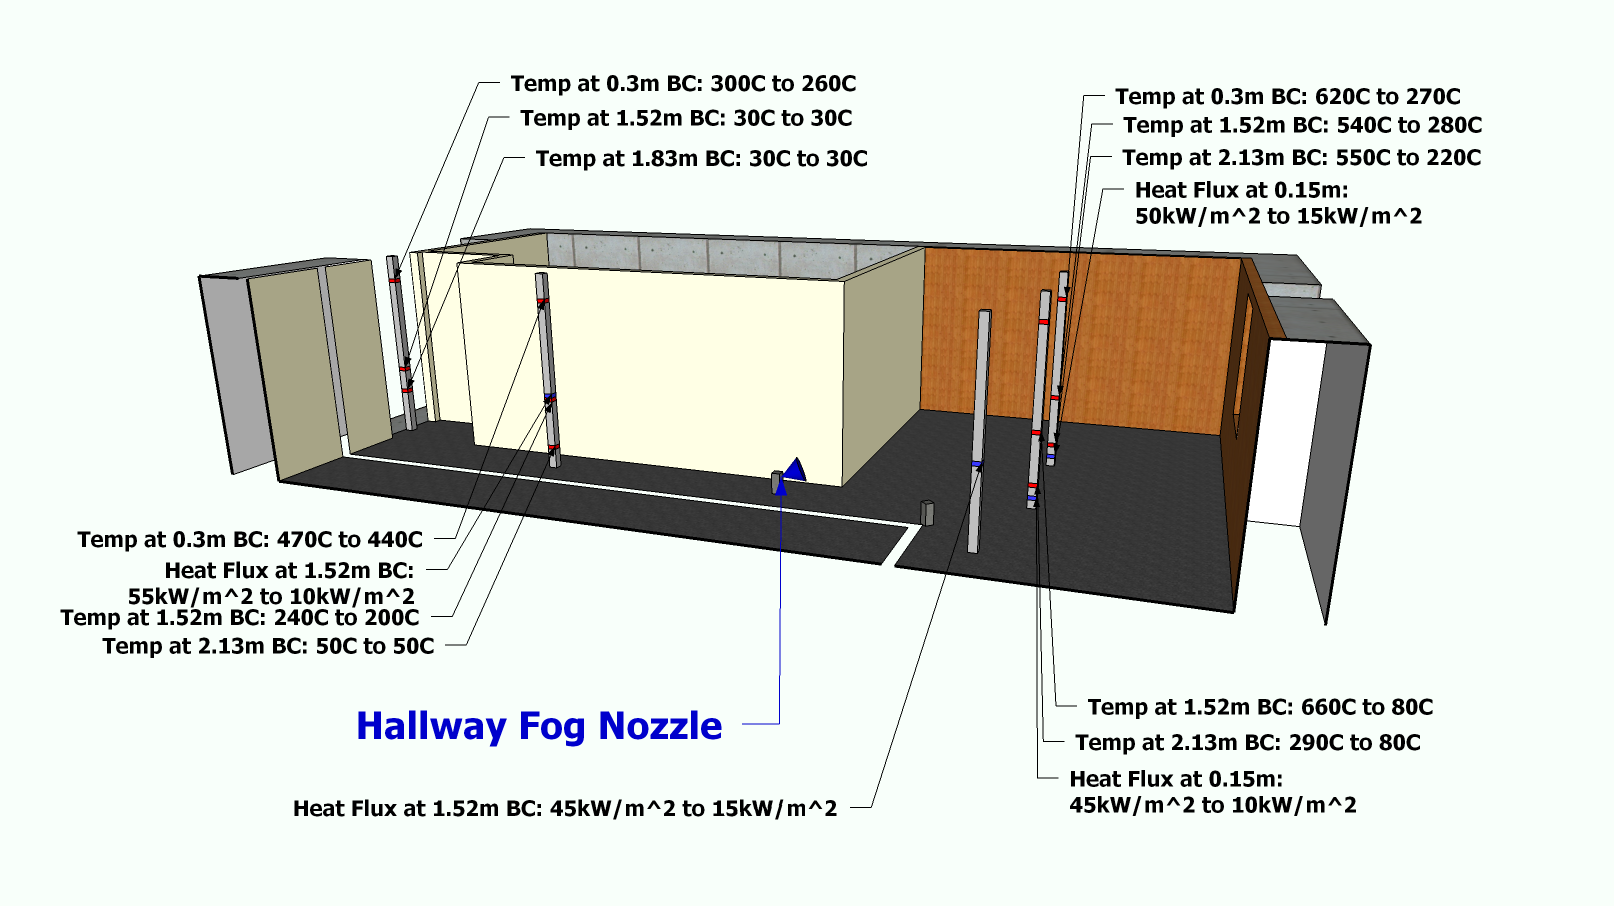
\includegraphics[width=6in]{../Figures/Pictures/Metric/DelCoFogTest8FirstSuppression}
	\caption{Test 8: Furniture Fuel Package, CAFS, 30 deg Fog, 120 gpm/60cfm, First Suppression}
	\label{fig:Test_8_First_Suppression}
\end{figure}

\begin{figure}[!ht]
	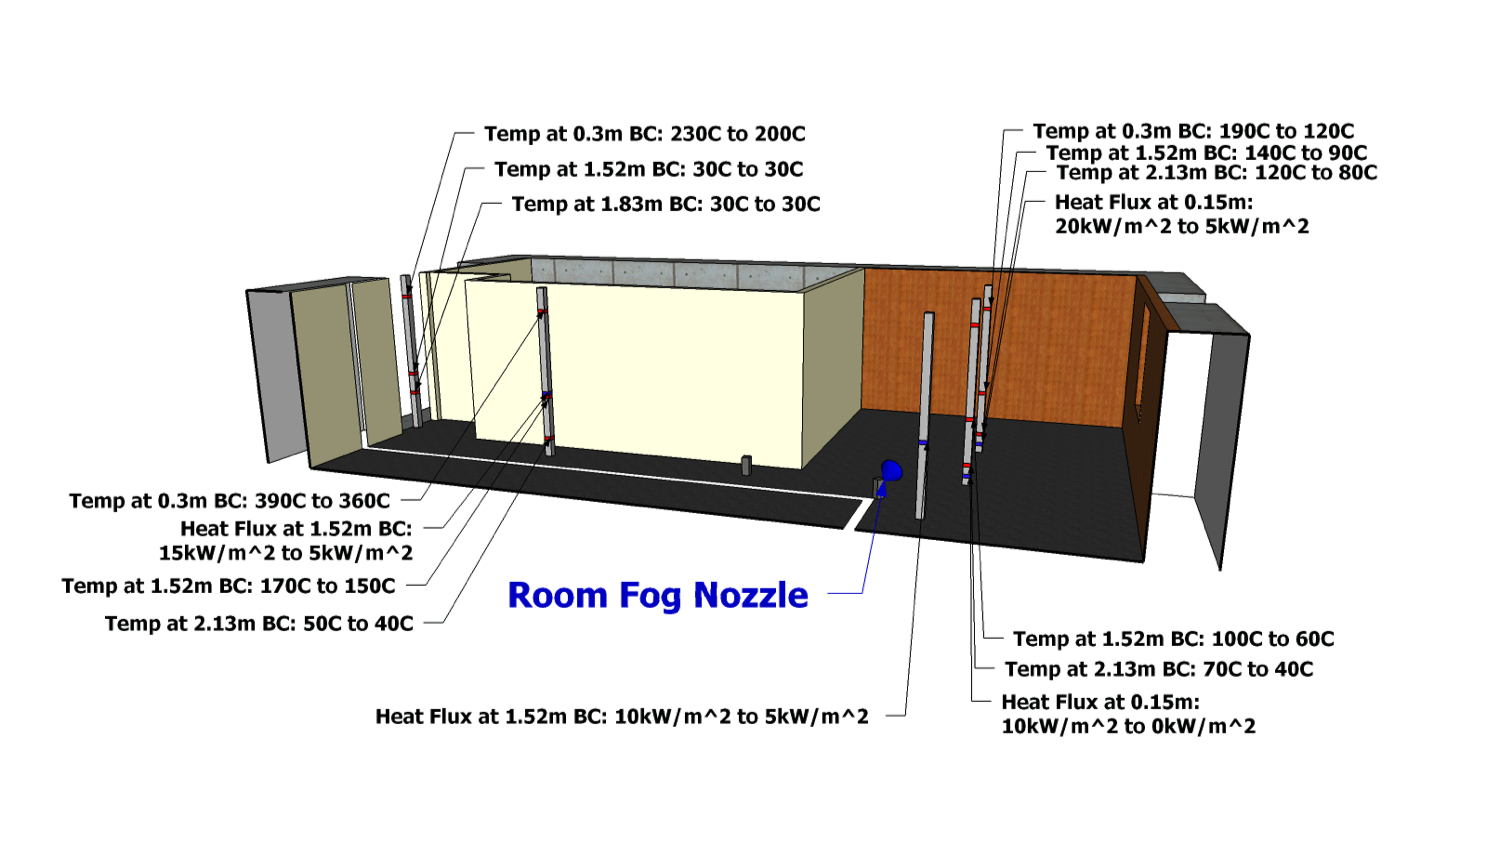
\includegraphics[width=6in]{../Figures/Pictures/Metric/DelCoFogTest8SecondSuppression}
	\caption{Test 8: Furniture Fuel Package, CAFS, 30 deg Fog, 120 gpm/60cfm, Second Suppression}
	\label{fig:Test_8_Second_Suppression}
\end{figure}

\subsection{Spray Density}
\label{subsec:Spray_Density}
	
\chapter{Discussion and Tactical Considerations}
\label{chap:Discussion_and_Tactical_Considerations}

\chapter{Summary}
\label{chap:Summary}

\chapter{Appendix}
\label{chap:Appendix}

\section{Test 1 Figures}
\label{subsec:Test_1_Figures}

\subsection{Temperature}
\label{subsec:Temperature}

\begin{figure}[!ht]
	\includegraphics[width=6in]{../Figures/Temperature/FSE1_Eastside_Array}
	\caption{Test 1 (FSE1): Eastside Array}
	\label{fig:Test_1_Eastside_Array}
\end{figure}

\begin{figure}[!ht]
	\includegraphics[width=6in]{../Figures/Temperature/FSE1_Westside_Array}
	\caption{Test 1 (FSE1): Westside Array}
	\label{fig:Test_1_Westside_Array}
\end{figure}

\begin{figure}[!ht]
	\includegraphics[width=6in]{../Figures/Temperature/FSE1_Hallway_Array}
	\caption{Test 1 (FSE1): Hallway Array}
	\label{fig:Test_1_Hallway_Array}
\end{figure}

\begin{figure}[!ht]
	\includegraphics[width=6in]{../Figures/Temperature/FSE1_Doorway_Array}
	\caption{Test 1 (FSE1): Doorway Array}
	\label{fig:Test_1_Doorway_Array}
\end{figure}

\begin{figure}[!ht]
	\includegraphics[width=6in]{../Figures/Temperature/Suppression_FSE1_Eastside_Array}
	\caption{Test 1 (FSE1): Suppression Eastside Array}
	\label{fig:Test_1_Suppression_Eastside_Array}
\end{figure}

\begin{figure}[!ht]
	\includegraphics[width=6in]{../Figures/Temperature/Suppression_FSE1_Westside_Array}
	\caption{Test 1 (FSE1): Suppression Westside Array}
	\label{fig:Test_1_Suppression_Westside_Array}
\end{figure}

\begin{figure}[!ht]
	\includegraphics[width=6in]{../Figures/Temperature/Suppression_FSE1_Hallway_Array}
	\caption{Test 1 (FSE1): Suppression Hallway Array}
	\label{fig:Test_1_Suppression_Hallway_Array}
\end{figure}

\begin{figure}[!ht]
	\includegraphics[width=6in]{../Figures/Temperature/Suppression_FSE1_Doorway_Array}
	\caption{Test 1 (FSE1): Suppression Doorway Array}
	\label{fig:Test_1_Suppression_Doorway_Array}
\end{figure}

\subsection{Heat Flux}
\label{subsec:Heat_Flux}

\begin{figure}[!ht]
	\includegraphics[width=6in]{../Figures/Heat_Flux/FSE_Test_1_Heat_Flux_Eastside}
	\caption{Test 1 (FSE1): Eastside Heat Flux}
	\label{fig:Test_1_Eastside_Heat_Flux}
\end{figure}

\begin{figure}[!ht]
	\includegraphics[width=6in]{../Figures/Heat_Flux/FSE_Test_1_Heat_Flux_Westside}
	\caption{Test 1 (FSE1): Westside Heat Flux}
	\label{fig:Test_1_Westside_Heat_Flux}
\end{figure}

\begin{figure}[!ht]
	\includegraphics[width=6in]{../Figures/Heat_Flux/FSE_Test_1_Heat_Flux_Hallway}
	\caption{Test 1 (FSE1): Hallway Heat Flux}
	\label{fig:Test_1_Hallway_Heat_Flux}
\end{figure}

\begin{figure}[!ht]
	\includegraphics[width=6in]{../Figures/Heat_Flux/FSE_Test_1_Heat_Flux_Near_Fire_Room}
	\caption{Test 1 (FSE1): Heat Flux Near Fire Room}
	\label{fig:Test_1_Heat_Flux_Near_Fire_Room}
\end{figure}

\subsection{Velocity}
\label{subsec:Velocity}

\begin{figure}[!ht]
	\includegraphics[width=6in]{../Figures/Velocity/FSE_Test_1_Hallway_Velocity}
	\caption{Test 1 (FSE1): Hallway Velocity}
	\label{fig:Test_1_Hallway_Velocity}
\end{figure}

\begin{figure}[!ht]
	\includegraphics[width=6in]{../Figures/Velocity/FSE_Test_1_Doorway_Velocity}
	\caption{Test 1 (FSE1): Doorway Velocity}
	\label{fig:Test_1_Doorway_Velocity}
\end{figure}

\clearpage

\section{Test 2 Figures}
\label{subsec:Test_2_Figures}

\subsection{Temperature}
\label{subsec:Temperature}

\begin{figure}[!ht]
	\includegraphics[width=6in]{../Figures/Temperature/FSW2_Eastside_Array}
	\caption{Test 2 (FSW2): Eastside Array}
	\label{fig:Test_2_Eastside_Array}
\end{figure}

\begin{figure}[!ht]
	\includegraphics[width=6in]{../Figures/Temperature/FSW2_Westside_Array}
	\caption{Test 2 (FSW2: Westside Array}
	\label{fig:Test_2_Westside_Array}
\end{figure}

\begin{figure}[!ht]
	\includegraphics[width=6in]{../Figures/Temperature/FSW2_Hallway_Array}
	\caption{Test 2 (FSW2): Hallway Array}
	\label{fig:Test_2_Hallway_Array}
\end{figure}

\begin{figure}[!ht]
	\includegraphics[width=6in]{../Figures/Temperature/FSW2_Doorway_Array}
	\caption{Test 2 (FSW2): Doorway Array}
	\label{fig:Test_2_Doorway_Array}
\end{figure}

\begin{figure}[!ht]
	\includegraphics[width=6in]{../Figures/Temperature/Suppression_FSW2_Eastside_Array}
	\caption{Test 2 (FSW2): Suppression Eastside Array}
	\label{fig:Test_2_Suppression_Eastside_Array}
\end{figure}

\begin{figure}[!ht]
	\includegraphics[width=6in]{../Figures/Temperature/Suppression_FSW2_Westside_Array}
	\caption{Test 2 (FSW2): Suppression Westside Array}
	\label{fig:Test_2_Suppression_Westside_Array}
\end{figure}

\begin{figure}[!ht]
	\includegraphics[width=6in]{../Figures/Temperature/Suppression_FSW2_Hallway_Array}
	\caption{Test 2 (FSW2): Suppression Hallway Array}
	\label{fig:Test_2_Suppression_Hallway_Array}
\end{figure}

\begin{figure}[!ht]
	\includegraphics[width=6in]{../Figures/Temperature/Suppression_FSW2_Doorway_Array}
	\caption{Test 2 (FSW2): Suppression Doorway Array}
	\label{fig:Test_2_Suppression_Doorway_Array}
\end{figure}

\subsection{Heat Flux}
\label{subsec:Heat_Flux}

\begin{figure}[!ht]
	\includegraphics[width=6in]{../Figures/Heat_Flux/FSW_Test_2_Heat_Flux_Eastside}
	\caption{Test 2 (FSW2): Eastside Heat Flux}
	\label{fig:Test_2_Eastside_Heat_Flux}
\end{figure}

\begin{figure}[!ht]
	\includegraphics[width=6in]{../Figures/Heat_Flux/FSW_Test_2_Heat_Flux_Westside}
	\caption{Test 2 (FSW2): Westside Heat Flux}
	\label{fig:Test_2_Westside_Heat_Flux}
\end{figure}

\begin{figure}[!ht]
	\includegraphics[width=6in]{../Figures/Heat_Flux/FSW_Test_2_Heat_Flux_Hallway}
	\caption{Test 2 (FSW2): Hallway Heat Flux}
	\label{fig:Test_2_Hallway_Heat_Flux}
\end{figure}

\begin{figure}[!ht]
	\includegraphics[width=6in]{../Figures/Heat_Flux/FSW_Test_2_Heat_Flux_Near_Fire_Room}
	\caption{Test 2 (FSW2): Heat Flux Near Fire Room}
	\label{fig:Test_2_Heat_Flux_Near_Fire_Room}
\end{figure}

\subsection{Velocity}
\label{subsec:Velocity}

\begin{figure}[!ht]
	\includegraphics[width=6in]{../Figures/Velocity/FSW_Test_2_Hallway_Velocity}
	\caption{Test 2 (FSW2): Hallway Velocity}
	\label{fig:Test_2_Hallway_Velocity}
\end{figure}

\begin{figure}[!ht]
	\includegraphics[width=6in]{../Figures/Velocity/FSW_Test_2_Doorway_Velocity}
	\caption{Test 2 (FSW2): Doorway Velocity}
	\label{fig:Test_2_Doorway_Velocity}
\end{figure}

\clearpage

\section{Test 3 Figures}
\label{subsec:Test_3_Figures}

\subsection{Temperature}
\label{subsec:Temperature}

\begin{figure}[!ht]
	\includegraphics[width=6in]{../Figures/Temperature/FSW3_Eastside_Array}
	\caption{Test 3 (FSW3): Eastside Array}
	\label{fig:Test_3_Eastside_Array}
\end{figure}

\begin{figure}[!ht]
	\includegraphics[width=6in]{../Figures/Temperature/FSW3_Westside_Array}
	\caption{Test 3 (FSW3: Westside Array}
	\label{fig:Test_3_Westside_Array}
\end{figure}

\begin{figure}[!ht]
	\includegraphics[width=6in]{../Figures/Temperature/FSW3_Hallway_Array}
	\caption{Test 3 (FSW3): Hallway Array}
	\label{fig:Test_3_Hallway_Array}
\end{figure}

\begin{figure}[!ht]
	\includegraphics[width=6in]{../Figures/Temperature/FSW3_Doorway_Array}
	\caption{Test 3 (FSW3): Doorway Array}
	\label{fig:Test_3_Doorway_Array}
\end{figure}

\begin{figure}[!ht]
	\includegraphics[width=6in]{../Figures/Temperature/Suppression_FSW3_Eastside_Array}
	\caption{Test 3 (FSW3): Suppression Eastside Array}
	\label{fig:Test_3_Suppression_Eastside_Array}
\end{figure}

\begin{figure}[!ht]
	\includegraphics[width=6in]{../Figures/Temperature/Suppression_FSW3_Westside_Array}
	\caption{Test 3 (FSW3): Suppression Westside Array}
	\label{fig:Test_3_Suppression_Westside_Array}
\end{figure}

\begin{figure}[!ht]
	\includegraphics[width=6in]{../Figures/Temperature/Suppression_FSW3_Hallway_Array}
	\caption{Test 3 (FSW3): Suppression Hallway Array}
	\label{fig:Test_3_Suppression_Hallway_Array}
\end{figure}

\begin{figure}[!ht]
	\includegraphics[width=6in]{../Figures/Temperature/Suppression_FSW3_Doorway_Array}
	\caption{Test 3 (FSW3): Suppression Doorway Array}
	\label{fig:Test_3_Suppression_Doorway_Array}
\end{figure}

\subsection{Heat Flux}
\label{subsec:Heat_Flux}

\begin{figure}[!ht]
	\includegraphics[width=6in]{../Figures/Heat_Flux/FSW_Test_3_Heat_Flux_Eastside}
	\caption{Test 3 (FSW3): Eastside Heat Flux}
	\label{fig:Test_3_Eastside_Heat_Flux}
\end{figure}

\begin{figure}[!ht]
	\includegraphics[width=6in]{../Figures/Heat_Flux/FSW_Test_3_Heat_Flux_Westside}
	\caption{Test 3 (FSW3): Westside Heat Flux}
	\label{fig:Test_3_Westside_Heat_Flux}
\end{figure}

\begin{figure}[!ht]
	\includegraphics[width=6in]{../Figures/Heat_Flux/FSW_Test_3_Heat_Flux_Hallway}
	\caption{Test 3 (FSW3): Hallway Heat Flux}
	\label{fig:Test_3_Hallway_Heat_Flux}
\end{figure}

\begin{figure}[!ht]
	\includegraphics[width=6in]{../Figures/Heat_Flux/FSW_Test_3_Heat_Flux_Near_Fire_Room}
	\caption{Test 3 (FSW3): Heat Flux Near Fire Room}
	\label{fig:Test_3_Heat_Flux_Near_Fire_Room}
\end{figure}

\subsection{Velocity}
\label{subsec:Velocity}

\begin{figure}[!ht]
	\includegraphics[width=6in]{../Figures/Velocity/FSW_Test_3_Hallway_Velocity}
	\caption{Test 3 (FSW3): Hallway Velocity}
	\label{fig:Test_3_Hallway_Velocity}
\end{figure}

\begin{figure}[!ht]
	\includegraphics[width=6in]{../Figures/Velocity/FSW_Test_3_Doorway_Velocity}
	\caption{Test 3 (FSW3): Doorway Velocity}
	\label{fig:Test_3_Doorway_Velocity}
\end{figure}

\clearpage

\section{Test 4 Figures}
\label{subsec:Test_4_Figures}

\subsection{Temperature}
\label{subsec:Temperature}

\begin{figure}[!ht]
	\includegraphics[width=6in]{../Figures/Temperature/FSE4_Eastside_Array}
	\caption{Test 4 (FSE4): Eastside Array}
	\label{fig:Test_4_Eastside_Array}
\end{figure}

\begin{figure}[!ht]
	\includegraphics[width=6in]{../Figures/Temperature/FSE4_Westside_Array}
	\caption{Test 4 (FSE4): Westside Array}
	\label{fig:Test_4_Westside_Array}
\end{figure}

\begin{figure}[!ht]
	\includegraphics[width=6in]{../Figures/Temperature/FSE4_Hallway_Array}
	\caption{Test 4 (FSE4): Hallway Array}
	\label{fig:Test_4_Hallway_Array}
\end{figure}

\begin{figure}[!ht]
	\includegraphics[width=6in]{../Figures/Temperature/FSE4_Doorway_Array}
	\caption{Test 4 (FSE4): Doorway Array}
	\label{fig:Test_4_Doorway_Array}
\end{figure}

\begin{figure}[!ht]
	\includegraphics[width=6in]{../Figures/Temperature/Suppression_FSE4_Eastside_Array}
	\caption{Test 4 (FSE4): Suppression Eastside Array}
	\label{fig:Test_4_Suppression_Eastside_Array}
\end{figure}

\begin{figure}[!ht]
	\includegraphics[width=6in]{../Figures/Temperature/Suppression_FSE4_Westside_Array}
	\caption{Test 4 (FSE4): Suppression Westside Array}
	\label{fig:Test_4_Suppression_Westside_Array}
\end{figure}

\begin{figure}[!ht]
	\includegraphics[width=6in]{../Figures/Temperature/Suppression_FSE4_Hallway_Array}
	\caption{Test 4 (FSE4): Suppression Hallway Array}
	\label{fig:Test_4_Suppression_Hallway_Array}
\end{figure}

\begin{figure}[!ht]
	\includegraphics[width=6in]{../Figures/Temperature/Suppression_FSE4_Doorway_Array}
	\caption{Test 4 (FSE4): Suppression Doorway Array}
	\label{fig:Test_4_Suppression_Doorway_Array}
\end{figure}

\subsection{Heat Flux}
\label{subsec:Heat_Flux}

\begin{figure}[!ht]
	\includegraphics[width=6in]{../Figures/Heat_Flux/FSE_Test_4_Heat_Flux_Eastside}
	\caption{Test 4 (FSE4): Eastside Heat Flux}
	\label{fig:Test_4_Eastside_Heat_Flux}
\end{figure}

\begin{figure}[!ht]
	\includegraphics[width=6in]{../Figures/Heat_Flux/FSE_Test_4_Heat_Flux_Westside}
	\caption{Test 4 (FSE4): Westside Heat Flux}
	\label{fig:Test_4_Westside_Heat_Flux}
\end{figure}

\begin{figure}[!ht]
	\includegraphics[width=6in]{../Figures/Heat_Flux/FSE_Test_4_Heat_Flux_Hallway}
	\caption{Test 4 (FSE4): Hallway Heat Flux}
	\label{fig:Test_4_Hallway_Heat_Flux}
\end{figure}

\begin{figure}[!ht]
	\includegraphics[width=6in]{../Figures/Heat_Flux/FSE_Test_4_Heat_Flux_Near_Fire_Room}
	\caption{Test 4 (FSE4): Heat Flux Near Fire Room}
	\label{fig:Test_4_Heat_Flux_Near_Fire_Room}
\end{figure}

\subsection{Velocity}
\label{subsec:Velocity}

\begin{figure}[!ht]
	\includegraphics[width=6in]{../Figures/Velocity/FSE_Test_4_Hallway_Velocity}
	\caption{Test 4 (FSE4): Hallway Velocity}
	\label{fig:Test_4_Hallway_Velocity}
\end{figure}

\begin{figure}[!ht]
	\includegraphics[width=6in]{../Figures/Velocity/FSE_Test_4_Doorway_Velocity}
	\caption{Test 4 (FSE4): Doorway Velocity}
	\label{fig:Test_4_Doorway_Velocity}
\end{figure}

\clearpage

\section{Test 5 Figures}
\label{subsec:Test_5_Figures}

\subsection{Temperature}
\label{subsec:Temperature}

\begin{figure}[!ht]
	\includegraphics[width=6in]{../Figures/Temperature/FSE5_Eastside_Array}
	\caption{Test 5 (FSE5): Eastside Array}
	\label{fig:Test_5_Eastside_Array}
\end{figure}

\begin{figure}[!ht]
	\includegraphics[width=6in]{../Figures/Temperature/FSE5_Westside_Array}
	\caption{Test 5 (FSE5): Westside Array}
	\label{fig:Test_5_Westside_Array}
\end{figure}

\begin{figure}[!ht]
	\includegraphics[width=6in]{../Figures/Temperature/FSE5_Hallway_Array}
	\caption{Test 5 (FSE5): Hallway Array}
	\label{fig:Test_5_Hallway_Array}
\end{figure}

\begin{figure}[!ht]
	\includegraphics[width=6in]{../Figures/Temperature/FSE5_Doorway_Array}
	\caption{Test 5 (FSE5): Doorway Array}
	\label{fig:Test_5_Doorway_Array}
\end{figure}

\begin{figure}[!ht]
	\includegraphics[width=6in]{../Figures/Temperature/Suppression_FSE5_Eastside_Array}
	\caption{Test 5 (FSE5): Suppression Eastside Array}
	\label{fig:Test_5_Suppression_Eastside_Array}
\end{figure}

\begin{figure}[!ht]
	\includegraphics[width=6in]{../Figures/Temperature/Suppression_FSE5_Westside_Array}
	\caption{Test 5 (FSE5): Suppression Westside Array}
	\label{fig:Test_5_Suppression_Westside_Array}
\end{figure}

\begin{figure}[!ht]
	\includegraphics[width=6in]{../Figures/Temperature/Suppression_FSE5_Hallway_Array}
	\caption{Test 5 (FSE5): Suppression Hallway Array}
	\label{fig:Test_5_Suppression_Hallway_Array}
\end{figure}

\begin{figure}[!ht]
	\includegraphics[width=6in]{../Figures/Temperature/Suppression_FSE5_Doorway_Array}
	\caption{Test 5 (FSE5): Suppression Doorway Array}
	\label{fig:Test_5_Suppression_Doorway_Array}
\end{figure}

\subsection{Heat Flux}
\label{subsec:Heat_Flux}

\begin{figure}[!ht]
	\includegraphics[width=6in]{../Figures/Heat_Flux/FSE_Test_5_Heat_Flux_Eastside}
	\caption{Test 5 (FSE5): Eastside Heat Flux}
	\label{fig:Test_5_Eastside_Heat_Flux}
\end{figure}

\begin{figure}[!ht]
	\includegraphics[width=6in]{../Figures/Heat_Flux/FSE_Test_5_Heat_Flux_Westside}
	\caption{Test 5 (FSE5): Westside Heat Flux}
	\label{fig:Test_5_Westside_Heat_Flux}
\end{figure}

\begin{figure}[!ht]
	\includegraphics[width=6in]{../Figures/Heat_Flux/FSE_Test_5_Heat_Flux_Hallway}
	\caption{Test 5 (FSE5): Hallway Heat Flux}
	\label{fig:Test_5_Hallway_Heat_Flux}
\end{figure}

\begin{figure}[!ht]
	\includegraphics[width=6in]{../Figures/Heat_Flux/FSE_Test_5_Heat_Flux_Near_Fire_Room}
	\caption{Test 5 (FSE5): Heat Flux Near Fire Room}
	\label{fig:Test_5_Heat_Flux_Near_Fire_Room}
\end{figure}

\subsection{Velocity}
\label{subsec:Velocity}

\begin{figure}[!ht]
	\includegraphics[width=6in]{../Figures/Velocity/FSE_Test_5_Hallway_Velocity}
	\caption{Test 5 (FSE5): Hallway Velocity}
	\label{fig:Test_5_Hallway_Velocity}
\end{figure}

\begin{figure}[!ht]
	\includegraphics[width=6in]{../Figures/Velocity/FSE_Test_5_Doorway_Velocity}
	\caption{Test 5 (FSE5): Doorway Velocity}
	\label{fig:Test_5_Doorway_Velocity}
\end{figure}

\clearpage

\section{Test 6 Figures}
\label{subsec:Test_6_Figures}

\subsection{Temperature}
\label{subsec:Temperature}

\begin{figure}[!ht]
	\includegraphics[width=6in]{../Figures/Temperature/FSW6_Eastside_Array}
	\caption{Test 6 (FSW6): Eastside Array}
	\label{fig:Test_6_Eastside_Array}
\end{figure}

\begin{figure}[!ht]
	\includegraphics[width=6in]{../Figures/Temperature/FSW6_Westside_Array}
	\caption{Test 6 (FSW6: Westside Array}
	\label{fig:Test_6_Westside_Array}
\end{figure}

\begin{figure}[!ht]
	\includegraphics[width=6in]{../Figures/Temperature/FSW6_Hallway_Array}
	\caption{Test 6 (FSW6): Hallway Array}
	\label{fig:Test_6_Hallway_Array}
\end{figure}

\begin{figure}[!ht]
	\includegraphics[width=6in]{../Figures/Temperature/FSW6_Doorway_Array}
	\caption{Test 6 (FSW6): Doorway Array}
	\label{fig:Test_6_Doorway_Array}
\end{figure}

\begin{figure}[!ht]
	\includegraphics[width=6in]{../Figures/Temperature/Suppression_FSW6_Eastside_Array}
	\caption{Test 6 (FSW6): Suppression Eastside Array}
	\label{fig:Test_6_Suppression_Eastside_Array}
\end{figure}

\begin{figure}[!ht]
	\includegraphics[width=6in]{../Figures/Temperature/Suppression_FSW6_Westside_Array}
	\caption{Test 6 (FSW6): Suppression Westside Array}
	\label{fig:Test_6_Suppression_Westside_Array}
\end{figure}

\begin{figure}[!ht]
	\includegraphics[width=6in]{../Figures/Temperature/Suppression_FSW6_Hallway_Array}
	\caption{Test 6 (FSW6): Suppression Hallway Array}
	\label{fig:Test_6_Suppression_Hallway_Array}
\end{figure}

\begin{figure}[!ht]
	\includegraphics[width=6in]{../Figures/Temperature/Suppression_FSW6_Doorway_Array}
	\caption{Test 6 (FSW6): Suppression Doorway Array}
	\label{fig:Test_6_Suppression_Doorway_Array}
\end{figure}

\subsection{Heat Flux}
\label{subsec:Heat_Flux}

\begin{figure}[!ht]
	\includegraphics[width=6in]{../Figures/Heat_Flux/FSW_Test_6_Heat_Flux_Eastside}
	\caption{Test 6 (FSW6): Eastside Heat Flux}
	\label{fig:Test_6_Eastside_Heat_Flux}
\end{figure}

\begin{figure}[!ht]
	\includegraphics[width=6in]{../Figures/Heat_Flux/FSW_Test_6_Heat_Flux_Westside}
	\caption{Test 6 (FSW6): Westside Heat Flux}
	\label{fig:Test_6_Westside_Heat_Flux}
\end{figure}

\begin{figure}[!ht]
	\includegraphics[width=6in]{../Figures/Heat_Flux/FSW_Test_6_Heat_Flux_Hallway}
	\caption{Test 6 (FSW6): Hallway Heat Flux}
	\label{fig:Test_6_Hallway_Heat_Flux}
\end{figure}

\begin{figure}[!ht]
	\includegraphics[width=6in]{../Figures/Heat_Flux/FSW_Test_6_Heat_Flux_Near_Fire_Room}
	\caption{Test 6 (FSW6): Heat Flux Near Fire Room}
	\label{fig:Test_6_Heat_Flux_Near_Fire_Room}
\end{figure}

\subsection{Velocity}
\label{subsec:Velocity}

\begin{figure}[!ht]
	\includegraphics[width=6in]{../Figures/Velocity/FSW_Test_6_Hallway_Velocity}
	\caption{Test 6 (FSW6): Hallway Velocity}
	\label{fig:Test_6_Hallway_Velocity}
\end{figure}

\begin{figure}[!ht]
	\includegraphics[width=6in]{../Figures/Velocity/FSW_Test_6_Doorway_Velocity}
	\caption{Test 6 (FSW6): Doorway Velocity}
	\label{fig:Test_6_Doorway_Velocity}
\end{figure}

\clearpage

\section{Test 7 Figures}
\label{subsec:Test_7_Figures}

\subsection{Temperature}
\label{subsec:Temperature}

\begin{figure}[!ht]
	\includegraphics[width=6in]{../Figures/Temperature/FSW7_Eastside_Array}
	\caption{Test 7 (FSW7): Eastside Array}
	\label{fig:Test_7_Eastside_Array}
\end{figure}

\begin{figure}[!ht]
	\includegraphics[width=6in]{../Figures/Temperature/FSW7_Westside_Array}
	\caption{Test 7 (FSW7: Westside Array}
	\label{fig:Test_7_Westside_Array}
\end{figure}

\begin{figure}[!ht]
	\includegraphics[width=6in]{../Figures/Temperature/FSW7_Hallway_Array}
	\caption{Test 7 (FSW7): Hallway Array}
	\label{fig:Test_7_Hallway_Array}
\end{figure}

\begin{figure}[!ht]
	\includegraphics[width=6in]{../Figures/Temperature/FSW7_Doorway_Array}
	\caption{Test 7 (FSW7): Doorway Array}
	\label{fig:Test_7_Doorway_Array}
\end{figure}

\begin{figure}[!ht]
	\includegraphics[width=6in]{../Figures/Temperature/Suppression_FSW7_Eastside_Array}
	\caption{Test 7 (FSW7): Suppression Eastside Array}
	\label{fig:Test_7_Suppression_Eastside_Array}
\end{figure}

\begin{figure}[!ht]
	\includegraphics[width=6in]{../Figures/Temperature/Suppression_FSW7_Westside_Array}
	\caption{Test 7 (FSW7): Suppression Westside Array}
	\label{fig:Test_7_Suppression_Westside_Array}
\end{figure}

\begin{figure}[!ht]
	\includegraphics[width=6in]{../Figures/Temperature/Suppression_FSW7_Hallway_Array}
	\caption{Test 7 (FSW7): Suppression Hallway Array}
	\label{fig:Test_7_Suppression_Hallway_Array}
\end{figure}

\begin{figure}[!ht]
	\includegraphics[width=6in]{../Figures/Temperature/Suppression_FSW7_Doorway_Array}
	\caption{Test 7 (FSW7): Suppression Doorway Array}
	\label{fig:Test_7_Suppression_Doorway_Array}
\end{figure}

\subsection{Heat Flux}
\label{subsec:Heat_Flux}

\begin{figure}[!ht]
	\includegraphics[width=6in]{../Figures/Heat_Flux/FSW_Test_7_Heat_Flux_Eastside}
	\caption{Test 7 (FSW7): Eastside Heat Flux}
	\label{fig:Test_7_Eastside_Heat_Flux}
\end{figure}

\begin{figure}[!ht]
	\includegraphics[width=6in]{../Figures/Heat_Flux/FSW_Test_7_Heat_Flux_Westside}
	\caption{Test 7 (FSW7): Westside Heat Flux}
	\label{fig:Test_7_Westside_Heat_Flux}
\end{figure}

\begin{figure}[!ht]
	\includegraphics[width=6in]{../Figures/Heat_Flux/FSW_Test_7_Heat_Flux_Hallway}
	\caption{Test 7 (FSW7): Hallway Heat Flux}
	\label{fig:Test_7_Hallway_Heat_Flux}
\end{figure}

\begin{figure}[!ht]
	\includegraphics[width=6in]{../Figures/Heat_Flux/FSW_Test_7_Heat_Flux_Near_Fire_Room}
	\caption{Test 7 (FSW7): Heat Flux Near Fire Room}
	\label{fig:Test_7_Heat_Flux_Near_Fire_Room}
\end{figure}

\subsection{Velocity}
\label{subsec:Velocity}

\begin{figure}[!ht]
	\includegraphics[width=6in]{../Figures/Velocity/FSW_Test_7_Hallway_Velocity}
	\caption{Test 7 (FSW7): Hallway Velocity}
	\label{fig:Test_7_Hallway_Velocity}
\end{figure}

\begin{figure}[!ht]
	\includegraphics[width=6in]{../Figures/Velocity/FSW_Test_7_Doorway_Velocity}
	\caption{Test 7 (FSW7): Doorway Velocity}
	\label{fig:Test_7_Doorway_Velocity}
\end{figure}

\clearpage

\section{Test 8 Figures}
\label{subsec:Test_8_Figures}

\subsection{Temperature}
\label{subsec:Temperature}

\begin{figure}[!ht]
	\includegraphics[width=6in]{../Figures/Temperature/FSE8_Eastside_Array}
	\caption{Test 8 (FSE8): Eastside Array}
	\label{fig:Test_8_Eastside_Array}
\end{figure}

\begin{figure}[!ht]
	\includegraphics[width=6in]{../Figures/Temperature/FSE8_Westside_Array}
	\caption{Test 8 (FSE8): Westside Array}
	\label{fig:Test_8_Westside_Array}
\end{figure}

\begin{figure}[!ht]
	\includegraphics[width=6in]{../Figures/Temperature/FSE8_Hallway_Array}
	\caption{Test 8 (FSE8): Hallway Array}
	\label{fig:Test_8_Hallway_Array}
\end{figure}

\begin{figure}[!ht]
	\includegraphics[width=6in]{../Figures/Temperature/FSE8_Doorway_Array}
	\caption{Test 8 (FSE8): Doorway Array}
	\label{fig:Test_8_Doorway_Array}
\end{figure}

\begin{figure}[!ht]
	\includegraphics[width=6in]{../Figures/Temperature/Suppression_FSE8_Eastside_Array}
	\caption{Test 8 (FSE8): Suppression Eastside Array}
	\label{fig:Test_8_Suppression_Eastside_Array}
\end{figure}

\begin{figure}[!ht]
	\includegraphics[width=6in]{../Figures/Temperature/Suppression_FSE8_Westside_Array}
	\caption{Test 8 (FSE8): Suppression Westside Array}
	\label{fig:Test_8_Suppression_Westside_Array}
\end{figure}

\begin{figure}[!ht]
	\includegraphics[width=6in]{../Figures/Temperature/Suppression_FSE8_Hallway_Array}
	\caption{Test 8 (FSE8): Suppression Hallway Array}
	\label{fig:Test_8_Suppression_Hallway_Array}
\end{figure}

\begin{figure}[!ht]
	\includegraphics[width=6in]{../Figures/Temperature/Suppression_FSE8_Doorway_Array}
	\caption{Test 8 (FSE8): Suppression Doorway Array}
	\label{fig:Test_8_Suppression_Doorway_Array}
\end{figure}

\subsection{Heat Flux}
\label{subsec:Heat_Flux}

\begin{figure}[!ht]
	\includegraphics[width=6in]{../Figures/Heat_Flux/FSE_Test_8_Heat_Flux_Eastside}
	\caption{Test 8 (FSE8): Eastside Heat Flux}
	\label{fig:Test_8_Eastside_Heat_Flux}
\end{figure}

\begin{figure}[!ht]
	\includegraphics[width=6in]{../Figures/Heat_Flux/FSE_Test_8_Heat_Flux_Westside}
	\caption{Test 8 (FSE8): Westside Heat Flux}
	\label{fig:Test_8_Westside_Heat_Flux}
\end{figure}

\begin{figure}[!ht]
	\includegraphics[width=6in]{../Figures/Heat_Flux/FSE_Test_8_Heat_Flux_Hallway}
	\caption{Test 8 (FSE8): Hallway Heat Flux}
	\label{fig:Test_8_Hallway_Heat_Flux}
\end{figure}

\begin{figure}[!ht]
	\includegraphics[width=6in]{../Figures/Heat_Flux/FSE_Test_8_Heat_Flux_Near_Fire_Room}
	\caption{Test 8 (FSE8): Heat Flux Near Fire Room}
	\label{fig:Test_8_Heat_Flux_Near_Fire_Room}
\end{figure}

\subsection{Velocity}
\label{subsec:Velocity}

\begin{figure}[!ht]
	\includegraphics[width=6in]{../Figures/Velocity/FSE_Test_8_Hallway_Velocity}
	\caption{Test 8 (FSE8): Hallway Velocity}
	\label{fig:Test_8_Hallway_Velocity}
\end{figure}

\begin{figure}[!ht]
	\includegraphics[width=6in]{../Figures/Velocity/FSE_Test_8_Doorway_Velocity}
	\caption{Test 8 (FSE8): Doorway Velocity}
	\label{fig:Test_8_Doorway_Velocity}
\end{figure}

\clearpage

\chapter{References}
\label{chap:References}

\bibliography{../../../Bibliography/FDS_refs,../../../Bibliography/FDS_general,references}

	
\end{document}

